\documentclass[letterpaper,11pt,x11names,english,french]{memoir}
  \usepackage{natbib,url,bibentry}
  \usepackage{babel}
  \usepackage[autolanguage]{numprint}
  \usepackage{amsmath,amsthm}
  \usepackage[shortlabels]{enumitem}
  \usepackage{textpos}
  \usepackage{graphicx}
  \usepackage{framed}                  % environnement titled-frame
  \usepackage{manfnt}                  % \mantriangleright (puce)
  \usepackage{dirtree}                 % arbre pour exercice sur \include
  \usepackage{metalogo}                % \XeLaTeX logo
  \usepackage{fontawesome}             % plusieurs icônes
  \usepackage{answers}                 % exercices et solutions
  \usepackage{listings}                % code informatique
  \usepackage{pdfpages}                % couvertures

  %%% ===================
  %%%  Style du document
  %%% ===================

  %% Polices de caractères
  \usepackage{fontspec}
  \usepackage[bold-style=ISO]{unicode-math}
  \defaultfontfeatures{Scale=0.92}
  \setmainfont[Ligatures=TeX,Numbers=OldStyle]{Lucida Bright OT}
  \setmathfont{Lucida Bright Math OT}
  \setmonofont{Lucida Grande Mono DK}
  \setsansfont[Scale=1.0,Numbers=OldStyle]{Myriad Pro}
  \newfontfamily\fullcaps[Letters=Uppercase,Numbers=Uppercase]{Myriad Pro}
  \usepackage[babel=true]{microtype}
  \usepackage{icomma}

  %% Polices additionnelles pour le chapitre trucs et astuces
  \newfontfamily\CM{cmunrm.otf}                       % Computer Modern
  \newfontfamily\Times{texgyretermes-regular.otf}     % Times
  \newfontfamily\Palatino{texgyrepagella-regular.otf} % Palatino

  %% Couleurs
  \usepackage{xcolor}
  \definecolor{comments}{rgb}{0.7,0,0}    % rouge foncé
  \definecolor{link}{rgb}{0,0.4,0.6}      % ~RoyalBlue de dvips
  \definecolor{url}{rgb}{0.6,0,0}         % rouge-brun
  \definecolor{citation}{rgb}{0,0.5,0}    % vert foncé
  \definecolor{ULlinkcolor}{rgb}{0,0,0.3} % de ulthese.cls

  %% Hyperliens
  \usepackage{hyperref}
  \hypersetup{colorlinks, linktocpage,
    urlcolor=url, linkcolor=link, citecolor=citation,
    bookmarksopen, bookmarksnumbered, bookmarksdepth=subsubsection,
    pdftitle={Rédaction de thèses et mémoires avec LaTeX - Partie II},
    pdfauthor={Université Laval}}
  \setlength{\XeTeXLinkMargin}{1pt}

  %% Étiquettes de \autoref (redéfinitions compatibles avec babel).
  %% Attention! Les % à la fin des lignes sont importants sinon des
  %% blancs apparaissent dès que la commande \selectlanguage est
  %% utilisée, notamment dans la bibliographie.
  \addto\extrasfrench{%
    \def\subsectionautorefname{section}%
    \def\figureautorefname{figure}%
    \def\tableautorefname{tableau}%
    \def\exempleautorefname{exemple}%
    \def\exerciceautorefname{exercice}%
  }

  %% Table des matières (inspirée de classicthesis.sty)
  \renewcommand{\cftchapterleader}{\hspace{1.5em}}
  \renewcommand{\cftchapterafterpnum}{\cftparfillskip}
  \renewcommand{\cftsectionleader}{\hspace{1.5em}}
  \renewcommand{\cftsectionafterpnum}{\cftparfillskip}

  %% Titres des chapitres
  \chapterstyle{hangnum}
  \renewcommand{\chaptitlefont}{\normalfont\Huge\sffamily\bfseries\raggedright}

  %% Marges, entêtes et pieds de page
  \setlength{\marginparsep}{7mm}
  \setlength{\marginparwidth}{20mm}
  \setlength{\headwidth}{\textwidth}
  \addtolength{\headwidth}{\marginparsep}
  \addtolength{\headwidth}{\marginparwidth}
  \addtolength{\marginparwidth}{15mm} % plus d'espace pour titres de documentation

  %% Titres des sections et sous-sections
  \setsecheadstyle{\normalfont\Large\sffamily\bfseries\raggedright}
  \setsubsecheadstyle{\normalfont\large\sffamily\bfseries\raggedright}
  \maxsecnumdepth{subsection}
  \setsecnumdepth{subsection}

  %% Listes. Paramétrage avec enumitem.
  \setlist[enumerate]{leftmargin=*,align=left}
  \setlist[enumerate,2]{label=\alph*),labelsep=*,leftmargin=1.5em}
  \setlist[enumerate,3]{label=\roman*),labelsep=*,leftmargin=1.5em,align=right}
  \setlist[itemize]{leftmargin=*,align=left}

  %% Paramétrage de babel
  \frenchbsetup{CompactItemize=false,%
    ThinSpaceInFrenchNumbers=true,
    ItemLabeli=\mantriangleright,
    ItemLabelii=\textendash}
  \def\frenchfigurename{{\scshape Fig.}}
  \def\frenchtablename{{\scshape Tab.}}

  %% Sections de code source
  \lstloadlanguages{[LaTeX]TeX}
  \lstset{language=[LaTeX]TeX,
    basicstyle=\ttfamily\NoAutoSpacing,
    keywordstyle=\mdseries,
    commentstyle=\color{comments}\slshape,
    escapeinside=`',
    extendedchars=true,
    showstringspaces=false,
    backgroundcolor=\color{LightYellow1},
    frame=lr, rulecolor=\color{LightYellow1},
    xleftmargin=3.4pt, xrightmargin=3.4pt}

  %%% =========================
  %%%  Nouveaux environnements
  %%% =========================

  %% Exemples
  \theoremstyle{definition}
  \newtheorem{exemple}{Exemple}[chapter]

  %% Exercices et réponses
  \Newassociation{sol}{solution}{solutions}
  \newcounter{exercice}[chapter]
  \renewcommand{\theexercice}{\thechapter.\arabic{exercice}}
  \newenvironment{exercice}[1][]{%
    \begin{list}{}{%
        \refstepcounter{exercice}
        \ifthenelse{\equal{#1}{nosol}}{%
          \renewcommand{\makelabel}{\bfseries\theexercice}}{%
          \hypertarget{ex:\theexercice}{}
          \Writetofile{solutions}{\protect\hypertarget{sol:\theexercice}{}}
          \renewcommand{\makelabel}{%
            \bfseries\protect\hyperlink{sol:\theexercice}{\theexercice}}}
        \settowidth{\labelwidth}{\bfseries\theexercice}
        \setlength{\leftmargin}{\labelwidth}
        \addtolength{\leftmargin}{\labelsep}
        \setlist[enumerate,1]{label=\alph*),labelsep=*,leftmargin=1.5em}
        \setlist[enumerate,2]{label=\roman*),labelsep=0.5em,align=right}}
      \item}
    {\end{list}}
  \renewenvironment{solution}[1]{%
    \begin{list}{}{%
        \renewcommand{\makelabel}{%
          \bfseries\protect\hyperlink{ex:#1}{#1}}
        \settowidth{\labelwidth}{\bfseries #1}
        \setlength{\leftmargin}{\labelwidth}
        \addtolength{\leftmargin}{\labelsep}
        \setlist[enumerate,1]{label=\alph*),labelsep=*,leftmargin=1.5em}
        \setlist[enumerate,2]{label=\roman*),labelsep=0.5em,align=right}}
      \item}
    {\end{list}}

  %% Démo de code LaTeX. Le code de 'texample' et 'eqxample' est
  %% repris de amsldoc.tex avec des petits ajustements.
  \newenvironment{demo}{%
    \begin{trivlist}\item}{%
    \end{trivlist}}
  \newenvironment{texample}[1][0.5\linewidth]{%
    \noindent\begin{minipage}{#1}%
      \def\producing{\end{minipage}\hfill\begin{minipage}{\dimexpr0.97\linewidth-#1}%
        \hbox\bgroup\kern-.2pt%
        \vbox\bgroup\parindent0pt\relax
        % The 3pt is to cancel the -\lineskip from \displ@y
        \abovedisplayskip3pt \abovedisplayshortskip\abovedisplayskip
        \belowdisplayskip0pt \belowdisplayshortskip\belowdisplayskip
        \noindent}
    }{%
      \par
      % Ensure that a lonely \[\] structure doesn't take up width less than
      % \hsize.
      \hrule height0pt width\hsize
      \egroup\kern-.2pt\egroup
    \end{minipage}%
    \par
  }
  \newenvironment{eqxample}{%
    \noindent\begin{minipage}{.5\columnwidth}%
      \def\producing{\end{minipage}\hfill\begin{minipage}{.45\columnwidth}%
        \hbox\bgroup\kern-.2pt\vrule width.2pt%
        \vbox\bgroup\parindent0pt\relax
        % The 3pt is to cancel the -\lineskip from \displ@y
        \abovedisplayskip3pt \abovedisplayshortskip\abovedisplayskip
        \belowdisplayskip0pt \belowdisplayshortskip\belowdisplayskip
        \noindent}
    }{%
      \par
      % Ensure that a lonely \[\] structure doesn't take up width less than
      % \hsize.
      \hrule height0pt width\hsize
      \egroup\vrule width.2pt\kern-.2pt\egroup
    \end{minipage}%
    \par
  }

  %% Un exemple du chapitre Trucs et astuces nécessite des
  %% environnements 'lstlisting' imbriqués, ce que ne digère pas
  %% LaTeX. La ruse consiste à définir un environnement équivalent qui
  %% porte simplement un autre nom.
  \lstnewenvironment{vglisting}{}{}

  %% Exemples de notices bibliographiques
  \newenvironment{bibexample}[1][\linewidth]{%
    \begin{minipage}[t]{#1}%
      \begin{trivlist}}
      {\end{trivlist}\end{minipage}}

  %% Encadré générique pour les remarques importantes et autres
  %% comportant une icône sur la gauche. Argument: symbole à
  %% placer sur la gauche (obligatoire).
  \newenvironment{infobox}[1]{%
    \setlength{\FrameRule}{1pt}
    \begin{table}[h]%
      \begin{framed}%
        \noindent
        \begin{minipage}{0.1\linewidth}
          \raisebox{-1.5em}[0em][0em]{\HUGE#1}
        \end{minipage}
        \begin{minipage}[t]{0.88\linewidth}}%
        {\end{minipage}\end{framed}\end{table}}

  %% Remarques importantes
  \newenvironment{important}{%
    \begin{infobox}{\faExclamationCircle}}%
    {\end{infobox}}

  %% Informations
  \newenvironment{information}{%
    \begin{infobox}{\faInfoCircle}}%
    {\end{infobox}}

  %% Encadré avec titre (basé sur 'titled-frame' de framed pour les
  %% conseils du TeXpert. Cet environnement est laissé flottant.
  \newenvironment{conseil}{%
    \colorlet{TFFrameColor}{black}%
    \colorlet{TFTitleColor}{white}%
    \begin{table}%
      \begin{titled-frame}{\sffamily Conseil du {\TeX}pert}%
        \noindent
        \begin{minipage}{0.1\linewidth}
          \raisebox{-1.5em}[0em][0em]{\HUGE\faThumbsOUp}
        \end{minipage}
        \begin{minipage}[t]{0.88\linewidth}}%
        {\end{minipage}\end{titled-frame}\end{table}}

  %%% =======
  %%%  Index
  %%% =======
  \renewcommand{\preindexhook}{%
    Cet index contient des références aux commandes et environnements
    {\LaTeX}, ainsi qu'aux noms de paquetages et de classes.%
    \vskip\onelineskip%
    Le premier numéro indique habituellement, mais pas toujours,
    la page où un concept est introduit, défini ou expliqué.%
    \vskip\onelineskip}
  \lstset{language=[LaTeX]TeX,
    morekeywords={align,align*,aligned,cases,center,equation,equation*,%
      figure,gather,lstlisting,minipage,multline,quote,split,%
      table,tabular,tabularx,verbatim},
    moretexcs={toprule,midrule,bottomrule,%
      includegraphics,reflectbox,resizebox,rotatebox,scalebox,%
      includepdf,frenchfigurename,frenchtablename,%
      newsubfloat,subcaption,%
      dfrac,tfrac,iint,text,mathcal,mathbb,eqref,symbf,%
      citet,citep,citeauthor,citeyear,%
      setmainfont,setmathfont,%
      color,definecolor,colorlet,hypersetup},
    deletetexcs={documentclass,usepackage,begin,end,LaTeX,TeX,%
      bfseries,emph,Huge,itshape,normalfont,raggedright,sffamily,small,textbf,texttt,%
      minipage,hfill,def,a,b,c,d,em,i,j,l,r,t},
    index=[1][keywords],        % environnements
    indexstyle=[1]\ixenv,
    index=[2][texcs],           % commandes
    indexstyle=[2]\ixcmd}
  \newcommand{\ixenv}[1]{\index{#1 env@\Pe{#1} (environnement)}%
    \index{environnement!#1@\Pe{#1}}}
  \newcommand{\ixcmd}[1]{\index{#1@\string\cs{#1}}}
  \makeindex

  %%% =====================
  %%%  Nouvelles commandes
  %%% =====================

  %% Noms de fonctions, code, environnement, etc.
  \newcommand{\code}[1]{\texttt{#1}}
  \newcommand{\fichier}[1]{\texttt{#1}}
  \newcommand{\class}[1]{\textsf{#1}\index{#1 class@\textsf{#1} (classe)}%
    \index{classe!#1}}
  \newcommand{\pkg}[1]{\textbf{#1}\index{#1 pkg@\textbf{#1} (paquetage)}%
    \index{paquetage!#1}}
  \newcommand{\Pe}[1]{\code{#1}}         % tiré de la doc de memoir
  \newcommand{\Ie}[1]{\Pe{#1}\ixenv{#1}} % idem
  \newcommand{\mat}[1]{\symbf{#1}}       % en mode mathématique

  %% Modification de commandes tirées de memoir.cls servant à afficher
  %% des noms de commandes.
  %% - \cmdprint est modifiée pour que le nom de la commande ne soit
  %%   pas en italique;
  %% - \cmd est modifiée pour utiliser @ comme séparateur dans \index
  %%   et pour utiliser \cs plutôt que \cmdprint pour afficher le nom de
  %%   la commande (afin d'obtenir le même format d'entrée d'index
  %%   qu'avec \indexcmd ci-dessus).
  \renewcommand{\cmdprint}[1]{\textup{\texttt{\string#1}}}
  \makeatletter
  \renewcommand{\cmd}[1]{\cmdprint{#1}%
    \index{\expandafter\@gobble\string#1@\string\cs{\expandafter\@gobble\string#1}}}
  \makeatother

  %% Indications de capsule vidéo dans la marge
  \newcommand{\capsule}[2]{\href{#1}{#2}\marginpar{%
      \href{#1}{\raisebox{-0.5em}[0em][0em]{\HUGE\faYoutubePlay}}}}

  %% Hyperlien avec symbole de lien externe juste après
  \newcommand{\link}[2]{\href{#1}{#2~\raisebox{-0.2ex}{\faExternalLink}}}

  %% Lien vers documentation dans la marge
  %% usage: \doc[documentation]{nom_fichier}{url}
  \newcommand{\doc}[3][documentation]{\link{#3}{#1}%
    \ifthenelse{\equal{#2}{}}{}{\marginpar%
      [\hfill\faBook~\fichier{#2}]%
      {\faBook~\fichier{#2}}}}

  %% Suppression de l'hyperlien
  \newcommand{\nolink}[1]{\begin{NoHyper}#1\end{NoHyper}}

  %% «Bouton» de la page de copyright
  \newcommand{\browsebutton}{%
    \setlength{\fboxrule}{1pt}%
    \framebox[40mm][l]{%
      \rule[-5pt]{0mm}{16pt}%
      \makebox[7mm]{\raisebox{-3pt}{\LARGE\faExternalLink}}\;%
      {\sffamily Accéder au dépôt}}}

  %% Pour le tableau des commandes d'espacement en mode mathématique.
  %% Pris de la doc de amsmath.
  \newcommand{\lspx}{\mathord{\dashv\mkern-3mu}}
  \newcommand{\rspx}{\mathord{\mkern-2mu\vdash}}
  \newcommand{\spx}[1]{$\lspx #1\rspx$}

  %% Logo BIBTeX; tiré de http://bit.ly/1RQqUnG
  \newcommand{\BibTeX}{\rmfamily B\kern-.05em{\scshape i\kern-.025em b}\kern-.08em \TeX}

  %% Chapitre sur les bibliographies: des références bibliographiques
  %% sont insérées dans le texte avec \bibentry. Certaines commandes
  %% de francaisbst.tex sont alors utilisées, mais non encore
  %% définies. Répétées ici. De plus, il faut définir ici la commande
  %% \enquote plutôt que dans francais.bst. C'est pourquoi il y a une
  %% version modifiée de ce fichier dans ces sources.
  %% Voir http://bit.ly/1MORZmp
  \global\def\bbland{et}
  \global\def\bbledn{\'ed.}
  \global\def\bblfourtho{4{\ieme}}
  \global\def\bblth{{\ieme}}
  \global\def\bblvol{vol.}
  \def\bblno{\no{}}
  \def\bblpp{p.}
  \newcommand{\enquote}[1]{\guillemotleft#1\guillemotright}

  %%% =======
  %%%  Varia
  %%% =======

  %% Style de la bibliographie
  \bibliographystyle{francais}

  %% Aide pour la césure
  \hyphenation{}

  %%% ======================================
  %%%  Page titre (sauf titre de la partie)
  %%% ======================================
  \renewcommand{\year}{2016}
  \title{\protect\raggedright
    \mdseries\fontsize{32}{33}\selectfont Rédaction de thèses \\
                                          et de mémoires \\
                                          avec
    \bfseries\fontsize{62}{33}\selectfont \raisebox{-0.75ex}{\LaTeX} \\[10mm]
    \mdseries\fontsize{18}{24}\selectfont 2. Concepts avancés}
  % \author{\protect\raggedright
  %   \bfseries\fontsize{16}{20}\selectfont Vincent Goulet}
  % \date{%
  %   \mdseries\fontsize{14}{18}\selectfont Notes de cours \textbar\
  %                                         Exercices \textemdash\
  %                                         édition \year}

%  \includeonly{trucs}

\begin{document}

\frontmatter

\pagestyle{empty}

\maketitle

% %% Page couverture avant. Il faut modifier la largeur des graphiques
% %% puisque Sweave la règle à 0.8\textwidth.
% \setkeys{Gin}{width=\paperwidth}
% 
\includepdf[pages=1]{couvertures-partie_1}
% \setkeys{Gin}{width=0.8\textwidth}
% \cleardoublepage

% \include{pagegarde}
% \clearpage

\begingroup
\calccentering{\unitlength}
\begin{adjustwidth*}{\unitlength}{-\unitlength}
  \setlength{\parindent}{0pt}
  \setlength{\parskip}{\baselineskip}

  {\textcopyright} {\year} Université Laval \\

  
\includegraphics[height=7mm,keepaspectratio=true]{by-sa}\\%
  Cette création est mise à disposition selon le contrat
  \href{http://creativecommons.org/licenses/by-sa/4.0/deed.fr}{%
    Attribution-Partage dans les mêmes conditions 4.0 International} de
  Creative Commons. En vertu de ce contrat, vous êtes libre de:
  \begin{itemize}
  \item \textbf{partager} --- reproduire, distribuer et communiquer
    l'{\oe}uvre;
  \item \textbf{remixer} --- adapter l'{\oe}uvre;
  \item utiliser cette {\oe}uvre à des fins commerciales.
  \end{itemize}
  Selon les conditions suivantes:

  \begin{tabularx}{\linewidth}{@{}lX@{}}
    \raisebox{-9mm}[0mm][13mm]{%
    
\includegraphics[height=11mm,keepaspectratio=true]{by}}
    & \textbf{Attribution} --- Vous devez créditer l'{\oe}uvre, intégrer
      un lien vers le contrat et indiquer si des modifications ont été
      effectuées à l'{\oe}uvre. Vous devez indiquer ces informations par
      tous les moyens possibles, mais vous ne pouvez suggérer que
      l'Offrant vous soutient ou soutient la façon dont vous avez utilisé
      son {\oe}uvre. \\
    \raisebox{-9mm}{
\includegraphics[height=11mm,keepaspectratio=true]{sa}}
    & \textbf{Partage dans les mêmes conditions} --- Dans le cas où vous
      modifiez, transformez ou créez à partir du matériel composant
      l'{\oe}uvre originale, vous devez diffuser l'{\oe}uvre modifiée dans
      les même conditions, c'est à dire avec le même contrat avec lequel
      l'{\oe}uvre originale a été diffusée.
  \end{tabularx}
  \vspace*{4mm}

  Notes de cours et exercices développés par Vincent Goulet,
  professeur titulaire.
\end{adjustwidth*}
\endgroup

%%% Local Variables:
%%% mode: latex
%%% TeX-master: "formation_latex-partie_2"
%%% coding: utf-8
%%% End:

\clearpage

\pagestyle{companion}

%%% Copyright (C) 2018 Vincent Goulet
%%%
%%% Ce fichier fait partie du projet
%%% «Rédaction avec LaTeX»
%%% http://github.com/vigou3/formation-latex-ul
%%%
%%% Cette création est mise à disposition selon le contrat
%%% Attribution-Partage dans les mêmes conditions 4.0
%%% International de Creative Commons.
%%% http://creativecommons.org/licenses/by-sa/4.0/

\chapter{Introduction}
\label{chap:introduction}

Le présent ouvrage tire son origine d'une formation sur la rédaction
de thèses et de mémoires avec {\LaTeX} développée pour la Bibliothèque
de l'Université Laval. La formation aborde les concepts de base pour
un nouvel utilisateur: processus d'édition, compilation,
visualisation; séparation du contenu et de l'apparence du texte; mise
en forme du texte; séparation du document en parties; rudiments du
mode mathématique. Transformée en prose, la série de diapositives qui
appuie la présentation correspond grosso modo aux quatre premiers
chapitres de l'ouvrage.

Les six autres chapitres visent à rendre l'utilisateur de {\LaTeX}
débutant ou intermédiaire autonome dans la rédaction de documents
relativement complexes comportant des tableaux, des figures, des
équations mathématiques élaborées, une bibliographie, etc. Nous avons
aussi émaillé le texte de conseils et d'astuces glanés au fil de nos
vingt années d'utilisation du système de mise en page.

Les nombreuses références à la classe de documents \class{ulthese}
s'adressent au premier public de l'ouvrage: les étudiantes et
étudiants de l'Université Laval occupés à la rédaction de leur thèse
ou de leur mémoire. Ils devront utiliser cette classe pour composer un
document conforme aux règles générales de présentation matérielle de
la Faculté des études supérieures et postdoctorales. Les autres
lecteurs pourront sans mal escamoter ces passages.

Chaque chapitre comporte quelques exercices. Les solutions se trouvent
en annexe. En consultation électronique, le numéro d'un exercice est,
le cas échéant, un hyperlien vers sa solution, et vice versa.

Un index en fin d'ouvrage collige les références aux commandes et
environnements {\LaTeX}, ainsi qu'aux noms de paquetages et de
classes.

\subsection*{Autres références utiles}

L'ouvrage n'a aucune prétention d'exhaustivité. La consultation de
documentation additionnelle pourra s'avérer nécessaire pour réaliser
des mises en page plus élaborées. À cet égard, nous recommandons
chaudement le livre de \citet{Kopka:latex:4e} --- il a servi
d'inspiration pour ce document à maints endroits. La très complète
documentation (plus de 600~pages!) de la classe \class{memoir}
\citep{memoir} constitue une autre référence de choix. Nous
recommandons également:
\begin{itemize}
\item \link{http://fr.wikibooks.org/wiki/LaTeX}{\emph{LaTeX} dans
    Wikilivre} pour de la documentation en ligne, en français et
  libre;
\item le très actif forum de discussion
  \link{http://tex.stackexchange.com}{{\TeX}--{\LaTeX} Stack Exchange}
  (avant de penser y poser une question, vérifier que la réponse ne se trouve
  pas déjà dans le forum\dots\ ce qui risque fort d'être le cas);
\item la très complète
  \link{http://www.tex.ac.uk/cgi-bin/texfaq2html}{%
    \emph{foire aux questions}} (en anglais) du groupe des
  utilisateurs de {\LaTeX} du Royaume-Uni.
\end{itemize}

\subsection*{Installation d'une distribution}

L'utilisation de {\LaTeX} requiert évidemment une distribution du
système. Nous recommandons la distribution {\TeX}~Live administrée par
le {\TeX} Users Group. Les hyperliens ci-dessous mènent vers des
vidéos qui expliquent comment installer cette distribution.
\begin{itemize}
\item \capsule{https://youtu.be/kA53EQ3Q47w}{%
    Installation sur macOS}
\item \capsule{https://youtu.be/7MfodhaghUk}{%
    Installation sur Windows}
\end{itemize}

\subsection*{Hyperliens vers la documentation}

Le texte comporte plusieurs renvois vers la documentation d'un
paquetage ou d'une classe, par exemple vers la %
\doc{memoir}{http://texdoc.net/pkg/memoir/} %
de la classe \class{memoir}. L'hyperlien mène vers la version en ligne
de la documentation dans le site %
\link{http://texdoc.net}{TeXdoc Online}. On trouve également dans la
marge le nom du fichier correspondant (sans l'extension \code{.pdf})
sur un système doté de {\TeX}~Live.

La plupart des logiciels intégrés de rédaction {\LaTeX} offrent une
interface pour accéder à cette documentation.
\begin{itemize}
\item TeXShop: menu \code{Aide|Afficher l'aide pour le
    package} (\optkey\,\cmdkey\, I).
\item Texmaker: menu \code{Aide|TeXDoc [selection]}.
\item GNU~Emacs: commande \code{TeX-doc} (\code{C-c ?}) du mode
  spécialisé AUC{\TeX}.
\end{itemize}
Le lecteur devrait consulter la rubrique d'aide de son éditeur pour
savoir s'il offre une interface au système de gestion de la
documentation Texdoc de {\TeX}~Live.

\subsection*{Fichiers d'accompagnement}

Ce document devrait être accompagné des fichiers nécessaires pour
compléter certains exercices figurant à la fin des chapitres, ainsi
que d'un gabarit \fichier{exercice\_gabarit.tex} pour composer les
solutions des autres exercices. Si ce n'est pas le cas, récupérer les
fichiers dans le site \link{\ctanurl}{\emph{Comprehensive TeX Archive
    Network} (CTAN)}.

%%% Local Variables:
%%% mode: latex
%%% TeX-master: "formation-latex-ul"
%%% TeX-engine: xetex
%%% encoding: utf-8
%%% End:


\cleartorecto
\tableofcontents*

\mainmatter

\chapter{Document contenu dans plusieurs fichiers}
\label{chap:include}

Un document {\LaTeX} comporte toujours un préambule suivi du corps du
texte. Lorsque ceux-ci sont relativement courts (peu de commandes
spéciales et moins d'une vingtaine de pages de texte), il demeure
assez simple et convivial d'en faire l'édition dans un seul fichier à
l'aide de son éditeur de texte favori.

Cependant, si le préambule devient long et complexe ou, surtout,
lorsque l'ampleur du document augmente jusqu'à compter un grand nombre
de pages sur plusieurs chapitres, il convient de répartir les divers
éléments du document dans des fichiers séparés.

La segmentation en plusieurs fichiers rend l'édition du texte plus
simple et plus efficace. De plus, elle peut significativement
accélérer, durant la phase de rédaction, la compilation des documents
très longs ou comportant plusieurs images.


\section{Insertion de contenu avec la commande \cs{input}}
\label{sec:include:input}

La commande \cmd{\input} permet d'insérer le contenu d'un autre fichier
dans un document {\LaTeX}.
\begin{itemize}
\item La syntaxe de la commande est
\begin{lstlisting}
\input{`\textit{fichier}'}
\end{lstlisting}
  où le nom du fichier à insérer est \code{\textit{fichier}.tex}. On
  laisse donc tomber l'extension \verb=.tex= qui est implicite.
\item Le contenu du fichier est inséré tel quel dans le document,
  comme s'il avait été tapé dans le fichier qui contient l'appel à
  \cmd{\input}.
\item Le procédé est surtout utile pour sauvegarder séparément des
  bouts de code qui pourraient nuire à l'édition du texte (figures,
  longs tableaux) ou qui sont communs entre plusieurs documents
  (licence d'utilisation, auteur et affiliation).
\item La commande peut aussi être utilisée dans le préambule pour
  charger une partie ou l'ensemble de celui-ci. Cela permet de
  composer un même préambule pour plusieurs documents. Il
  suffit alors de faire d'éventuelles modifications à un seul endroit pour
  les voir prendre effet dans tous les documents.
\end{itemize}


\section{Insertion de parties avec la commande \cs{include}}
\label{sec:include:include}

Extrait de la documentation de la classe \class{ulthese}:
\begin{quote}
  «Il est recommandé de segmenter tout document d'une certaine ampleur
  dans des fichiers \verb=.tex= distincts pour chaque partie ---
  habituellement un fichier par chapitre. Le document complet est
  composé à l'aide d'un fichier maître qui contient le préambule
  {\LaTeX} et un ensemble de commandes \verb=\include= pour réunir les
  parties dans un tout.»
\end{quote}

Comme \cmd{\input}, la commande \cmd{\include} insère le contenu
d'un autre fichier dans un document {\LaTeX}. Son effet est cependant
différent et c'est son utilisation qui permet d'accélérer la
compilation d'un long document.

\begin{itemize}
\item L'insertion d'un fichier avec \cmd{\include} débute toujours
  une nouvelle page. On utilisera donc \cmd{\include} principalement
  pour insérer des chapitres entiers plutôt que pour des portions de
  texte.
\item Un fichier inséré avec \cmd{\include} peut contenir des appels
  à \cmd{\input}, mais pas à \cmd{\include}.
\item La syntaxe de la commande \cmd{\include} est
\begin{lstlisting}
\include{`\textit{fichier}'}
\end{lstlisting}
  où le nom du fichier à insérer est \code{\textit{fichier}.tex}. Ici
  aussi on laisse tomber l'extension \verb=.tex= qui est implicite.
\item La structure type d'un fichier maître est la suivante:
\begin{lstlisting}
\documentclass{ulthese}
  [...]

\begin{document}

\frontmatter

%%% Copyright (C) 2018 Vincent Goulet
%%%
%%% Ce fichier fait partie du projet
%%% «Rédaction avec LaTeX»
%%% http://github.com/vigou3/formation-latex-ul
%%%
%%% Cette création est mise à disposition selon le contrat
%%% Attribution-Partage dans les mêmes conditions 4.0
%%% International de Creative Commons.
%%% http://creativecommons.org/licenses/by-sa/4.0/

\chapter{Introduction}
\label{chap:introduction}

Le présent ouvrage tire son origine d'une formation sur la rédaction
de thèses et de mémoires avec {\LaTeX} développée pour la Bibliothèque
de l'Université Laval. La formation aborde les concepts de base pour
un nouvel utilisateur: processus d'édition, compilation,
visualisation; séparation du contenu et de l'apparence du texte; mise
en forme du texte; séparation du document en parties; rudiments du
mode mathématique. Transformée en prose, la série de diapositives qui
appuie la présentation correspond grosso modo aux quatre premiers
chapitres de l'ouvrage.

Les six autres chapitres visent à rendre l'utilisateur de {\LaTeX}
débutant ou intermédiaire autonome dans la rédaction de documents
relativement complexes comportant des tableaux, des figures, des
équations mathématiques élaborées, une bibliographie, etc. Nous avons
aussi émaillé le texte de conseils et d'astuces glanés au fil de nos
vingt années d'utilisation du système de mise en page.

Les nombreuses références à la classe de documents \class{ulthese}
s'adressent au premier public de l'ouvrage: les étudiantes et
étudiants de l'Université Laval occupés à la rédaction de leur thèse
ou de leur mémoire. Ils devront utiliser cette classe pour composer un
document conforme aux règles générales de présentation matérielle de
la Faculté des études supérieures et postdoctorales. Les autres
lecteurs pourront sans mal escamoter ces passages.

Chaque chapitre comporte quelques exercices. Les solutions se trouvent
en annexe. En consultation électronique, le numéro d'un exercice est,
le cas échéant, un hyperlien vers sa solution, et vice versa.

Un index en fin d'ouvrage collige les références aux commandes et
environnements {\LaTeX}, ainsi qu'aux noms de paquetages et de
classes.

\subsection*{Autres références utiles}

L'ouvrage n'a aucune prétention d'exhaustivité. La consultation de
documentation additionnelle pourra s'avérer nécessaire pour réaliser
des mises en page plus élaborées. À cet égard, nous recommandons
chaudement le livre de \citet{Kopka:latex:4e} --- il a servi
d'inspiration pour ce document à maints endroits. La très complète
documentation (plus de 600~pages!) de la classe \class{memoir}
\citep{memoir} constitue une autre référence de choix. Nous
recommandons également:
\begin{itemize}
\item \link{http://fr.wikibooks.org/wiki/LaTeX}{\emph{LaTeX} dans
    Wikilivre} pour de la documentation en ligne, en français et
  libre;
\item le très actif forum de discussion
  \link{http://tex.stackexchange.com}{{\TeX}--{\LaTeX} Stack Exchange}
  (avant de penser y poser une question, vérifier que la réponse ne se trouve
  pas déjà dans le forum\dots\ ce qui risque fort d'être le cas);
\item la très complète
  \link{http://www.tex.ac.uk/cgi-bin/texfaq2html}{%
    \emph{foire aux questions}} (en anglais) du groupe des
  utilisateurs de {\LaTeX} du Royaume-Uni.
\end{itemize}

\subsection*{Installation d'une distribution}

L'utilisation de {\LaTeX} requiert évidemment une distribution du
système. Nous recommandons la distribution {\TeX}~Live administrée par
le {\TeX} Users Group. Les hyperliens ci-dessous mènent vers des
vidéos qui expliquent comment installer cette distribution.
\begin{itemize}
\item \capsule{https://youtu.be/kA53EQ3Q47w}{%
    Installation sur macOS}
\item \capsule{https://youtu.be/7MfodhaghUk}{%
    Installation sur Windows}
\end{itemize}

\subsection*{Hyperliens vers la documentation}

Le texte comporte plusieurs renvois vers la documentation d'un
paquetage ou d'une classe, par exemple vers la %
\doc{memoir}{http://texdoc.net/pkg/memoir/} %
de la classe \class{memoir}. L'hyperlien mène vers la version en ligne
de la documentation dans le site %
\link{http://texdoc.net}{TeXdoc Online}. On trouve également dans la
marge le nom du fichier correspondant (sans l'extension \code{.pdf})
sur un système doté de {\TeX}~Live.

La plupart des logiciels intégrés de rédaction {\LaTeX} offrent une
interface pour accéder à cette documentation.
\begin{itemize}
\item TeXShop: menu \code{Aide|Afficher l'aide pour le
    package} (\optkey\,\cmdkey\, I).
\item Texmaker: menu \code{Aide|TeXDoc [selection]}.
\item GNU~Emacs: commande \code{TeX-doc} (\code{C-c ?}) du mode
  spécialisé AUC{\TeX}.
\end{itemize}
Le lecteur devrait consulter la rubrique d'aide de son éditeur pour
savoir s'il offre une interface au système de gestion de la
documentation Texdoc de {\TeX}~Live.

\subsection*{Fichiers d'accompagnement}

Ce document devrait être accompagné des fichiers nécessaires pour
compléter certains exercices figurant à la fin des chapitres, ainsi
que d'un gabarit \fichier{exercice\_gabarit.tex} pour composer les
solutions des autres exercices. Si ce n'est pas le cas, récupérer les
fichiers dans le site \link{\ctanurl}{\emph{Comprehensive TeX Archive
    Network} (CTAN)}.

%%% Local Variables:
%%% mode: latex
%%% TeX-master: "formation-latex-ul"
%%% TeX-engine: xetex
%%% encoding: utf-8
%%% End:

\tableofcontents*

\mainmatter
\include{historique}            % premier chapitre
\include{modele}                % deuxième chapitre
[...]

\end{document}
\end{lstlisting}
\end{itemize}

Le principal avantage de \cmd{\include} par rapport à \cmd{\input}
réside dans le fait que {\LaTeX} peut préserver entre les compilations
les informations telles que les numéros de pages, de sections ou
d'équations, ainsi que les références. Cela permet, par exemple, de
compiler le texte d'un seul chapitre --- plutôt que le document entier
--- et de néanmoins obtenir du chapitre une image représentative.
Procéder ainsi accélère significativement la compilation des documents
longs ou complexes.

\begin{itemize}
\item La commande \cmd{\includeonly}, que l'on utilise exclusivement
  dans le préambule, sert à spécifier le ou les fichiers à compiler
  tout en préservant la numérotation et les références. Sa syntaxe est
\begin{lstlisting}
\includeonly{`\textit{liste\_fichiers}'}
\end{lstlisting}
  où \code{\textit{liste\_fichiers}} contient les noms des fichiers à
  inclure dans la compilation, séparés par des virgules et sans
  l'extension \verb=.tex=.
\item Lors de l'utilisation de la commande \cmd{\includeonly}, toute
  la numérotation dans les fichiers \code{\textit{liste\_fichiers}}
  suivra celle établie lors de la compilation précédente.
\item Si l'édition des fichiers de \code{\textit{liste\_fichiers}}
  cause des changements dans la numérotation et les références dans
  les autres parties du document, une nouvelle compilation de
  l'ensemble ou d'une partie de celui-ci s'avérera nécessaire.
\end{itemize}

Supposons qu'un document est composé des fichiers
\verb=chapitre1.tex=, \verb=chapitre2.tex=, \verb=chapitre3.tex= et
que les chapitres débutent respectivement aux pages~1, 23 et 41.
\begin{itemize}
\item Si seul le fichier \verb=chapitre2.tex= est inclus dans la
  compilation, le numéro du chapitre sera toujours 2 et le folio de la
  première page sera toujours 23, même si les 22 pages précédentes ne se
  trouvent pas dans le document.
\item Si l'on modifie le fichier \verb=chapitre2= de telle sorte que
  le chapitre se termine maitenant à la page 46, il faudra recompiler
  le document avec au moins les fichiers \verb=chapitre2=  et
  \verb=chapitre3= pour que les pages du chapitre~3 soient renumérotées
  à partir de 47.
\end{itemize}

L'\autoref{ex:include} illustre mieux le cycle typique
d'utilisation des commandes \cmd{\include} et \cmd{\includeonly}.



%%%
%%% Exercices
%%%

\section{Exercices}
\label{sec:include:exercices}


\begin{exercice}
  \label{ex:include}
  Cet exercice fait appel au fichier maître
  \fichier{exercice\_include.tex} et à plusieurs fichiers auxiliaires.
  Schématiquement, le document est composé ainsi:

  \medskip
  \begin{minipage}{\linewidth}
    \dirtree{%
      .1 exercice\_include.tex.
      .2 {\textbackslash}input pagetitre.tex.
      .2 {\textbackslash}include presentation.tex.
      .3 {\textbackslash}includegraphics console-screenshot.pdf.
      .2 {\textbackslash}include emacs.tex.
    }
  \end{minipage}
  \medskip

  La commande \cmd{\includegraphics} permet d'insérer une image
  en divers formats (PDF, JPEG, PNG, \dots) dans un document {\LaTeX}.
  Elle provient du paquetage \pkg{graphicx}.

  \begin{enumerate}
  \item Étudier le code source du fichier maître
    \fichier{exercice\_include.tex}, puis le compiler deux à trois
    fois jusqu'à ce que toutes les références internes soient à jour.
    Il est normal à ce stade que la figure~1 du document soit vide.
  \item Ajouter dans le préambule du fichier maître la commande
\begin{lstlisting}
\includeonly{emacs}
\end{lstlisting}
    puis compiler le document.

    Observer que malgré l'absence du chapitre~1, la numérotation et
    les références demeurent à jour, notamment la table des matières.
  \item Remplacer la commande ajoutée en b) dans le préambule du
    fichier maître par la commande
\begin{lstlisting}
\includeonly{presentation}
\end{lstlisting}
    Vers la fin du fichier \fichier{presentation.tex}, activer la
    commande
\begin{lstlisting}
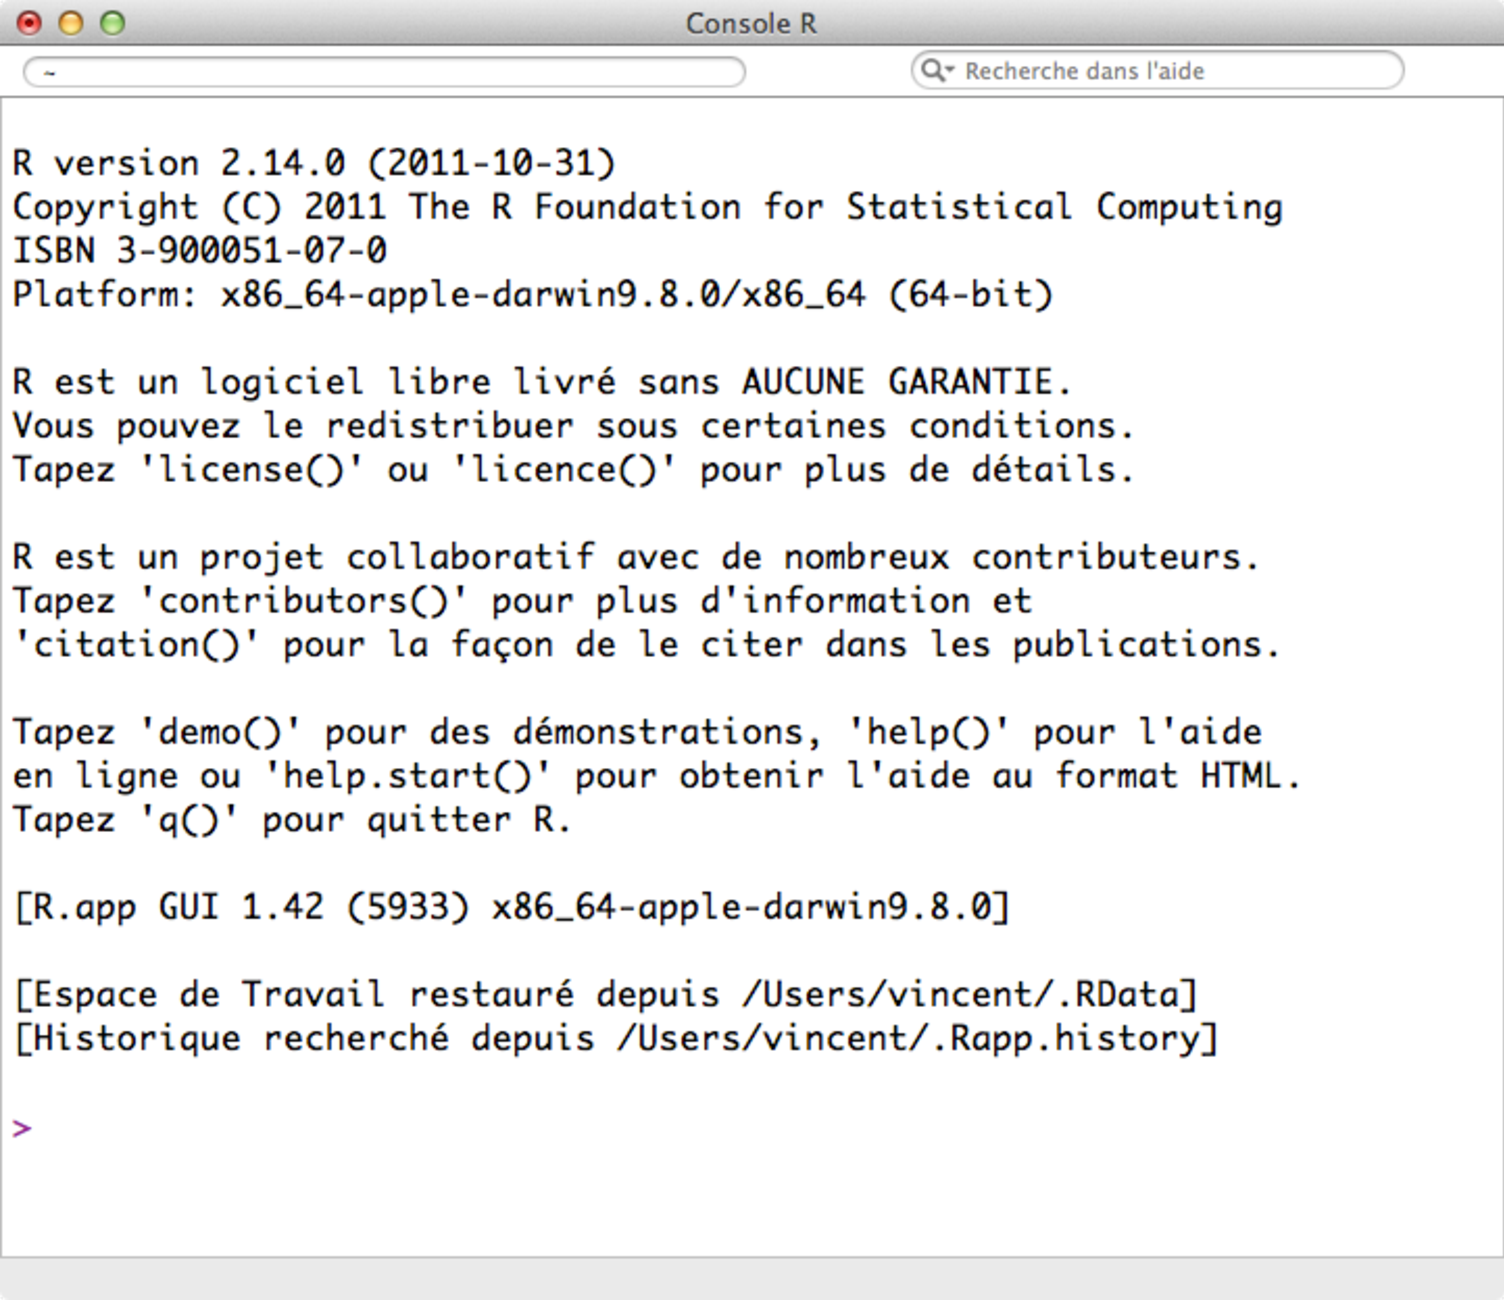
\includegraphics[width=\textwidth]{console-screenshot}
\end{lstlisting}
    en supprimant le symbole \% au début de la ligne. Compiler de
    nouveau le document deux fois.

    Les modifications ont eu pour effet d'ajouter une page au
    chapitre~1. Observer que selon la table des matières, le
    chapitre~2 débute toujours à la page~3 alors que celle-ci est
    maintenant occupée par la figure~1.
  \item Afin de corriger la table des matières, désactiver la
    commande \verb=\includeonly= dans le préambule du fichier maître,
    puis compiler de nouveau le document quelques fois.
  \end{enumerate}
\end{exercice}

\begin{exercice}
  Déplacer dans un fichier \fichier{preambule.tex} toutes les lignes
  du préambule du fichier \fichier{exercice\_include.tex} utilisé à
  l'exercice précédent, à l'exception de celles relatives à la page
  titre (titre, auteur, date). Insérer le préambule dans
  \fichier{exercice\_include.tex} avec la commande \cmd{\input}.
\end{exercice}

%%% Local Variables:
%%% mode: latex
%%% TeX-engine: xetex
%%% TeX-master: "formation_latex-partie_2"
%%% coding: utf-8
%%% End:

\chapter{Boîtes}
\label{chap:boites}

Il arrive que l'on doive traiter de manière spéciale une aire
rectangulaire de texte; pour l'encadrer, la mettre en surbrillance ou
la mettre en exergue, par exemple.

Avec les traitements de texte, on aura souvent recours aux tableaux à
de telles fins. Or, les tableaux devraient être réservés pour disposer
de l'information sous forme de lignes et de colonnes. (Un tableau
d'une seule cellule n'a donc pas vraiment de sens d'un point de vue
sémantique ou typographique.) Pour disposer et mettre en forme du tout
autre type contenu se présentant sous forme rectangulaire, {\LaTeX}
offre la solution plus générale des «boîtes».

Il existe trois sortes de boîtes en {\LaTeX}: les boîtes horizontales
dont le contenu est disposé exclusivement côte à côte; les boîtes
verticales qui peuvent contenir plusieurs lignes de contenu; les
boîtes de réglure pour former des lignes pleines de largeur et de
hauteur quelconques.

Il n'est pas inutile de savoir, au passage, que {\TeX} ne manipule que
cela, des boîtes. Pour {\TeX}, chaque caractère, chaque lettre n'est
qu'un rectangle d'une certaine largeur qui s'élève au-dessus de la
ligne de base (les lignes d'une feuille lignée) et qui, parfois, se
prolonge sous la ligne de base (pensons aux lettres \emph{p}, \emph{y}
ou \emph{Q}). Les commandes et environnements présentés ci-dessous
permettent simplement de créer d'autres boîtes dont le contrôle des
dimensions et du contenu est laissé à l'usager.

Une fois créée, une boîte ne peut être scindée en parties, notamment
entre les lignes ou entre les pages.



\section{Boîtes horizontales}
\label{sec:boites:lrbox}

Le plus simple concept de boîte dans {\LaTeX} est celui de boîte
«horizontale», c'est-à-dire dont le contenu est disposé latéralement
de gauche à droite\footnote{%
  D'où l'appellation \emph{LR (left-right) box} en anglais.}. %
Le contenu est normalement du texte, mais conceptuellement ce pourrait
être n'importe quoi, y compris d'autres boîtes.

Les commandes de base pour créer des boîtes horizontales sont:
\begin{lstlisting}
\mbox`\marg{texte}'
\fbox`\marg{texte}'
\end{lstlisting}
Elles produisent une boîte de la largeur précise de \meta{texte}. Avec
la commande \cmd{\fbox}, le texte est au surplus \fbox{encadré}. En
usage courant, la commande \cmd{\mbox} sert principalement à deux
choses:
\begin{enumerate}
\item réunir en un bloc du texte que l'on ne veut pas voir scindé
  entre les lignes ou entre les pages;
\item \label{item:tableaux:mbox} créer une boîte vide avec
  \cs{mbox\{\}} afin de laisser croire à {\TeX} que du contenu
  apparaît à un endroit, sans toutefois qu'il n'occupe aucun espace.
  %% ça prendrait un exemple de cela dans les exercices!
\end{enumerate}

Il existe également des versions plus générales des commandes
\cmd{\mbox} et \cmd{\fbox}:
\begin{lstlisting}
\makebox`\oarg{largeur}\oarg{pos}\marg{texte}'
\framebox`\oarg{largeur}\oarg{pos}\marg{texte}'
\end{lstlisting}
Les arguments optionnels \meta{largeur} et \meta{pos} déterminent
respectivement la largeur de la boîte et la position du texte
dans la boîte. Les valeurs possibles de \meta{pos} sont: \code{l} pour
du texte aligné à gauche, \code{r} pour du texte aligné à droite et
\code{c} (la valeur par défaut) pour du texte centré. Ainsi, la commande
\begin{lstlisting}
\framebox[3.5cm][l]{aligné à gauche}
\end{lstlisting}
produit \framebox[3.5cm][l]{aligné à gauche}, alors que
\begin{lstlisting}
\makebox[3.5cm]{centré}
\end{lstlisting}
produit \makebox[3.5cm]{centré}.



\section{Boîtes verticales}
\label{sec:boites:parbox}

Les boîtes verticales se distinguent des boîtes horizontales par le
fait qu'elles peuvent contenir plusieurs lignes de contenu empilées
les unes au-dessus des autres. Lorsque le contenu en question est du
texte, on obtient des paragraphes\footnote{%
  D'où l'appellation, cette fois, de \emph{paragraph boxes} en anglais
  ou \emph{parboxes} dans le jargon {\LaTeX}.}. %

La commande de base pour créer une boîte verticale est:
\begin{lstlisting}
\parbox`\oarg{pos}\marg{largeur}\marg{texte}'
\end{lstlisting}
Ici, l'argument optionnel \meta{pos} permet d'ajuster l'alignement
vertical de la boîte avec la ligne de base: \code{b} ou \code{t} selon
que l'on souhaite aligner, respectivement, le bas ou le haut de la
boîte avec la ligne de base. Par défaut, la boîte est centrée avec la
ligne de base. Cet argument n'a aucun effet si la boîte est le seul
élément de contenu du paragraphe.

On remarquera que l'argument \meta{largeur} est ici obligatoire.
Autrement dit, on doit nécessairement définir la largeur des boîtes
verticales, un peu comme il faut bien définir la largeur de la page
pour le texte normal.

Les boîtes créées avec \cmd{\parbox} ne peuvent contenir de structures
«complexes» comme des listes ou des tableaux. Parce que plus général,
l'outil véritablement utile pour la création de boîtes verticales est
l'environnement \Ie{minipage}. Cet environnement peut contenir à peu
n'importe quel type de contenu. Comme son nom l'indique, c'est ni plus
ni moins qu'une page miniature à l'intérieur de la page standard.

La syntaxe de l'environnement \Ie{minipage} est la suivante:
\begin{lstlisting}
\begin{minipage}`\oarg{pos}\marg{largeur}'
  `\meta{texte}'
\end{minipage}
\end{lstlisting}
La signification des arguments \meta{largeur} et \meta{pos} est la
même que pour la commande \cmd{parbox}.

L'environnement \Ie{minipage} est souvent utilisé pour disposer des
éléments de contenu de manière spécifique sur la page, notamment des
tableaux ou des figures côte à côte ou en grille (voir
l'\autoref{exemple:tableaux:grille} à la
\autopageref{exemple:tableaux:grille}).

\begin{exemple}
  Le code ci-dessous
\begin{lstlisting}
\begin{minipage}[b]{0.3\textwidth}
  La ligne inférieure de cette \emph{minipage} [...]
\end{minipage}
\hfill
\parbox{0.3\textwidth}{le centre de cette boîte [...] }
\hfill
\begin{minipage}[t]{0.3\textwidth}
  la ligne supérieure de cette \emph{minipage}. [...]
\end{minipage}
\end{lstlisting}
  produit: \\[0.5\baselineskip]
  \begin{minipage}{\textwidth}
    \makebox[0pt][l]{\color{lightgray}\rule{\textwidth}{0.7pt}}\relax
    \fbox{\begin{minipage}[b]{0.3\textwidth} La ligne inférieure de
        cette \emph{minipage} est alignée avec
      \end{minipage}} \hfill \fbox{\parbox{0.3\textwidth}{le centre de
        cette boîte verticale, qui est à son tour alignée avec}}
    \hfill \fbox{\begin{minipage}[t]{0.3\textwidth} la ligne
        supérieure de cette \emph{minipage}. Le filet horizontal grisé
        représente la ligne de base du paragraphe contenant les trois
        boîtes.
      \end{minipage}}
  \end{minipage}
  \qed
\end{exemple}

La commande \cmd{\hfill} utilisée entre les boîtes dans l'exemple
indique à {\LaTeX} d'insérer de l'espace blanc entre les éléments de
contenu de manière à remplir entièrement la ligne de texte. C'est une
commande très utile pour disposer automatiquement des éléments à
intervalles égaux sur la largeur du bloc de texte. Ainsi,
\begin{lstlisting}
\framebox[\textwidth]{gauche  \hfill droite}
\end{lstlisting}
produit \\[0.5\baselineskip]
\framebox[\textwidth]{gauche \hfill droite} \\[0.5\baselineskip]
alors que
\begin{lstlisting}
\framebox[\textwidth]{gauche \hfill centre \hfill droite.}
\end{lstlisting}
produit \\[0.5\baselineskip]
\framebox[\textwidth]{gauche \hfill centre \hfill droite.}



%%% Exercices: faire le contenu de 4.7.4 de Kopka et Daly (disposition
%%% verticale des boîtes)

\section{Boîtes de réglure}
\label{sec:boites:rulebox}

En imprimerie, une réglure est une ligne droite continue ou
pointillée. Une ligne n'étant jamais rien d'autre qu'un rectangle
plein, si mince fut-il, la réglure est le troisième type de
boîte\footnote{%
  \emph{Rule box}, en anglais} %
dans {\LaTeX}.

La commande
\begin{lstlisting}
\rule`\oarg{déplacement}\marg{largeur}\marg{hauteur}'
\end{lstlisting}
crée une réglure de dimensions \meta{largeur} $\times$ \meta{hauteur}.
Par défaut, la réglure s'appuie sur la ligne de base. Le résultat de
\begin{lstlisting}
\rule{2cm}{6pt}
\end{lstlisting}
est donc une ligne pleine de $2$~cm de long et de $6$~points d'épais:
\rule{2cm}{6pt}.

L'argument optionnel \meta{déplacement} permet de déplacer
verticalement la réglure au-dessus ou au-dessous de la ligne de base
selon que \meta{déplacement} est positif ou négatif. Avec les deux
commandes
\begin{lstlisting}
\rule[3pt]{2cm}{6pt}
\rule[-3pt]{2cm}{6pt}
\end{lstlisting}
on crée respectivement les réglures \rule[3pt]{2cm}{6pt} et
\rule[-3pt]{2cm}{6pt}.

Un usage intéressant de la réglure consiste à faire croire à {\TeX}
qu'une ligne est plus haute qu'il n'y parait en insérant dans celle-ci
une réglure de largeur nulle. Par exemple, la distance entre
\rule[-12pt]{0mm}{30pt}\relax la présente ligne et les autres du paragraphe est
plus grande que la normale parce que nous y avons inséré une réglure
invisible avec
\begin{lstlisting}
\rule[-12pt]{0mm}{30pt}
\end{lstlisting}
Ce truc est particulièrement utile pour augmenter la hauteur des
lignes dans un tableau; voir la \autoref{sec:tableaux:tableaux}.


%%% Local Variables:
%%% mode: latex
%%% TeX-engine: xetex
%%% TeX-master: "formation_latex-partie_2"
%%% coding: utf-8
%%% End:

\chapter{Tableaux et figures}
\label{chap:tableaux}

Les tableaux et graphiques ne sont pas les éléments de texte les plus
simples et rapides à créer avec {\LaTeX}. Les traitements de texte
brillent, ici, avec leurs interfaces graphiques permettant de composer
un tableau ou un graphique simple pièce par pièce avec la souris.

En revanche, pour ce type de contenu comme pour tout autre, {\LaTeX}
fait ce qu'on lui demande, sans tenter de deviner notre pensée ou,
pire, de prétendre savoir mieux que nous ce que nous voulons faire. À
ce chapitre, les traitements de texte ne brillent plus! Peut-être avez-vous
déjà eu de la difficulté à contrôler les bordures d'un tableau, la
hauteur des lignes ou la largeur des colonnes dans un traitement de
texte? Alors vous comprenez que l'exercice de composition d'un tableau
peut rapidement devenir frustrant.

Avant de discuter de la création ou de l'insertion de tableaux, de
graphiques et d'images dans un document {\LaTeX}, il convient de
présenter très succinctement quelques règles à suivre pour concevoir
des tableaux clairs et faciles à consulter.


\section{De la conception de beaux tableaux}
\label{sec:tableaux:booktabs}

On utilise les tableaux pour disposer de l'information sous forme de
grille. Par conséquent, le premier réflexe pour les mettre en forme
consiste souvent à mettre en évidence cette grille par le biais de
filets\footnote{%
  Terme typographique pour ce qui est communément appelés des «lignes»
  dans le langage courant ou des «bordures» dans les logiciels de
  traitement de texte. Dans la documentation en anglais, on parle de
  \emph{rules}.} %
horizontaux et verticaux.

C'est une mauvaise idée, une pratique à éviter. Vraiment!

Comparer les deux tableaux ci-dessous. Le premier est mis en forme
selon une approche classique supportée depuis toujours par {\LaTeX}:
filets doubles en entête et en pied de tableau, filets simples entre
chaque ligne et entre les colonnes.

\begin{center}
  \begin{tabular}{|>{$}c<{$}|>{$}r<{$}|>{$}r<{$}|>{$}r<{$}|>{$}c<{$}|>{$}c<{$}|}
    \hline\hline
    i &
    \multicolumn{1}{c|}{$v$} &
    \multicolumn{1}{c|}{$b_i$} &
    \lfloor v/b_i \rfloor & v \bmod b_i & x_i \\
    \hline
    0 & \nombre{91492} &  60 & \nombre{1524} & 52 & 52 \\
    \hline
    1 &  \nombre{1524} &  60 &           25  & 24 & 24 \\
    \hline
    2 &            25  &  24 &            1  &  1 &  1 \\
    \hline
    3 &             1  & 365 &            0  &  1 &  1 \\
    \hline\hline
  \end{tabular}
\end{center}

Le second tableau tire profit des fonctionnalités du paquetage
\pkg{booktabs} \citep{booktabs} et des recommandations de son auteur:
les filets horizontaux sont d'épaisseur différente selon qu'ils sont
situés dans l'entête et dans le pied du tableau ou entre les lignes,
l'espace autour des filets horizontaux est plus grand et, surtout, il
n'y a pas de filets verticaux.

\begin{center}
  \begin{tabular}{>{$}c<{$}>{$}r<{$}>{$}r<{$}>{$}r<{$}>{$}c<{$}>{$}c<{$}}
    \toprule
    i &
    \multicolumn{1}{c}{$v$} &
    \multicolumn{1}{c}{$b_i$} &
    \lfloor v/b_i \rfloor & v \bmod b_i & x_i \\
    \midrule
    0 & \nombre{91492} &  60 & \nombre{1524} & 52 & 52 \\
    1 &  \nombre{1524} &  60 &           25  & 24 & 24 \\
    2 &            25  &  24 &            1  &  1 &  1 \\
    3 &             1  & 365 &            0  &  1 &  1 \\
    \bottomrule
  \end{tabular}
\end{center}

La seconde version n'est-elle pas la plus aérée et la plus facile à
consulter? N'est-ce pas que, contrairement à ce que l'on pourrait
penser, les filets verticaux ne sont pas du tout requis pour bien
délimiter les colonnes?

Tel que mentionné ci-dessus, le paquetage \pkg{booktabs} ajoute des
fonctionnalités à {\LaTeX} pour améliorer la qualité typographique des
tableaux. Dans la %
\doc{booktabs}{http://texdoc.net/pkg/booktabs} %
du paquetage, son auteur énonce quelques règles à suivre pour la mise
en forme des tableaux:
\begin{enumerate}
\item ne \emph{jamais} utiliser de filets verticaux. Si l'information
  du côté gauche du tableau semble si différente de celle du côté
  droit qu'un filet vertical apparaît absolument nécessaire, scinder
  simplement l'information dans deux tableaux;
\item ne jamais utiliser de filets doubles;
\item placer les unités (\$, cm, {\textdegree}C, etc.) dans le titre
  de la colonne plutôt qu'après chaque valeur dans le corps du
  tableau;
\item toujours inscrire un chiffre du côté gauche du séparateur
  décimal: $0,1$ et non $,1$ (pratique plus répandue en anglais, où le
  séparateur décimal est le point);
\item ne pas utiliser un symbole pour représenter une valeur
  répétée (comme $''$ ou ---). Laisser un blanc ou répéter la
  valeur s'il subsiste une ambiguïté.
\end{enumerate}

Nous recommandons évidemment de suivre ces règles et c'est pourquoi la
présente documentation ainsi que les fichiers d'exemples font usage
des commandes de \pkg{booktabs}.

Les fonctionnalités de \pkg{booktabs} sont intégrées à la classe
\class{memoir} et, par conséquent, à \class{ulthese}. Il n'est donc pas
nécessaire de charger le paquetage avec ces deux classes.



\section{Tableaux}
\label{sec:tableaux:tableaux}

Peu importe l'outil informatique utilisé, la création d'un tableau
requiert toujours de préciser à l'ordinateur le nombre de colonnes que
contiendra le tableau, l'entête du tableau le cas échéant et le contenu
des différentes cellules. Cette dernière étape nécessite à son tour
une convention pour indiquer les passages à la colonne suivante
ainsi que le passage à la ligne suivante.

On crée des tableaux dans {\LaTeX} principalement avec les
environnements \Ie{tabular}, \Ie{tabular*} et \Ie{tabularx} (ce
dernier fourni par le paquetage \pkg{tabularx} ou par la classe
\class{memoir}). La syntaxe de ces environnements est:
\begin{lstlisting}
\begin{tabular}`\marg{format}'           `\textit{lignes}' \end{tabular}
\begin{tabular*}`\marg{largeur}\marg{format}' `\textit{lignes}' \end{tabular*}
\begin{tabularx}`\marg{largeur}\marg{format}' `\textit{lignes}' \end{tabularx}
\end{lstlisting}
La signification des arguments\footnote{%
  Nous avons omis un argument optionnel à peu près jamais utilisé
  servant à spécifier l'alignement vertical du tableau par rapport à
  la ligne de base externe.} %
est la suivante. Nous ne traitons ici que les options les plus souvent
employées. Pour une liste plus exhaustive, consulter la %
\doc{memman}{http://texdoc.net/pkg/memman} %
de la classe \class{memoir} (chapitre 11) ou %
\citet[section \link{http://fr.wikibooks.org/wiki/LaTeX/Tableaux}{Tableaux}]{wikilivres:latex}.

\begin{list}{}{%
    \setlength{\labelsep}{1.5ex}
    \settowidth{\labelwidth}{\meta{largeur}}
    \setlength{\leftmargin}{\labelwidth}
    \addtolength{\leftmargin}{\labelsep}
    \setlength{\parsep}{0.5ex plus0.2ex minus0.2ex}
    \setlength{\itemsep}{0.3ex}
    \renewcommand{\makelabel}[1]{\meta{#1}\hfill}}
%
\item[largeur] Largeur hors tout d'un tableau avec les environnements
  \Pe{tabular*} et \Pe{tabularx}. Autrement, avec l'environnement
  \Pe{tabular}, la largeur d'un tableau est déterminée automatiquement
  pour contenir tout le tableau, quitte à dépasser dans la marge de
  droite.

  La largeur du tableau est généralement exprimée en fraction de la
  largeur du bloc de texte. Celle-ci est accessible avec la commande
  \cs{textwidth}. Par exemple, les déclarations suivantes définissent
  respectivement des tableaux occupant toute la largeur d'une page et
  80~\% de la largeur de la page:
\begin{lstlisting}
\begin{tabular*}{\textwidth}`\marg{format}'
\end{lstlisting}
\begin{lstlisting}
\begin{tabularx}{0.8\textwidth}`\marg{format}'
\end{lstlisting}
  L'environnement \Ie{tabular*} joue sur l'espace entre les colonnes
  pour parvenir à la largeur prescrite, alors que \Ie{tabularx} joue
  sur la largeur des colonnes (voir ci-dessous).
  %
\item[format] Le format des colonnes et, par le fait même, le nombre
  de colonnes puisque l'argument doit compter un symbole pour chaque
  colonne du tableau. Les principaux symboles de mise en forme des
  colonnes sont:
  \begin{description}
  \item[\normalfont\code{l}] contenu de la colonne aligné à gauche;
  \item[\normalfont\code{r}] contenu de la colonne aligné à droite;
  \item[\normalfont\code{c}] contenu de la colonne centré;
  \item[\normalfont\code{p\{}\textit{lgr}\code{\}}] contenu de la colonne traité comme un
    paragraphe de texte de largeur \textit{lgr};
  \item[\normalfont\code{X}] [environnement \Pe{tabularx} seulement]
    colonne dont la largeur peut être ajustée pour obtenir un tableau
    de la largeur prescrite; identique à \code{p} par ailleurs.
  \end{description}
  Par exemple, la déclaration
\begin{lstlisting}
\begin{tabular}{lrp{5cm}}
\end{lstlisting}
  définit un tableau à trois colonnes dont le contenu de la première
  est aligné à gauche; celui de la seconde est aligné à droite; celui de
  la troisième est en texte libre dans une cellule de 5~cm de largeur.

  Avec la déclaration
\begin{lstlisting}
\begin{tabularx}{\textwidth}{lrX}
\end{lstlisting}
  la largeur de la troisième colonne sera plutôt adaptée
  automatiquement pour que le tableau occupe toute la largeur de la
  page.

  Les symboles \verb=|= et \verb=||= dans \textit{format} servent à
  insérer des filets verticaux simples et doubles entre les colonnes,
  mais nous avons vu à la \autoref{sec:tableaux:booktabs} que c'est
  une pratique à proscrire.
  %
\item[lignes] Le contenu des cellules du tableau. Les entrées des
  cellules sont séparées par le symbole \verb=&= et les lignes par
  {\bs\bs}. Une cellule peut être vide.

  Les lignes de contenu peuvent également contenir certaines commandes
  spéciales pour contrôler la mise en forme. La commande ci-dessous
  permet de fusionner des cellules:
  \begin{description}
  \item[\normalfont\cmdprint{\multicolumn\marg{num}\marg{fmt}\marg{texte}}]
    fusionne les \meta{num} cellules suivantes en une seule de format
    \meta{fmt} et contenant le texte \meta{texte}. \par%
    Cette commande ne peut apparaître qu'au début d'une ligne ou après
    un symbole de changement de colonne \verb=&=. \par%
    La commande est souvent utilisée avec une valeur de
    $\text{\meta{num}}$ égale à 1 pour changer le format d'une
    cellule, par exemple pour centrer le titre d'une colonne qui est autrement
    alignée à gauche ou à droite.
  \end{description}

  Les commandes suivantes\footnote{%
    Ce sont les commandes de \pkg{booktabs} et \class{memoir}
auxquelles nous faisions référence à la \autoref{sec:tableaux:booktabs}.} %
  servent à insérer des filets horizontaux dans un tableau:
  \begin{description}
  \item[\normalfont\cmd{\toprule}] insère un filet horizontal épais
    suivi d'un espace vertical au début d'un tableau;
  \item[\normalfont\cmd{\midrule}] insère un filet horizontal mince
    précédé et suivi d'un espace vertical entre deux lignes;
  \item[\normalfont\cmd{\cmidrule}\marg{m-n}] insère un filet
    horizontal comme \cmdprint{\midrule} de la gauche de la
    colonne \meta{m} à la droite de la colonne \meta{n};
  \item[\normalfont\cmd{\bottomrule}] insère un filet horizontal épais
    précédé d'un espace vertical à la fin d'un tableau.
  \end{description}
  Une fin de ligne {\bs\bs}  doit  obligatoirement précéder chacune
  de ces commandes, sauf évidemment \cmdprint{\toprule}.
\end{list}

La hauteur des lignes d'un tableau est déterminée automatiquement en
fonction du contenu de celles-ci.

\begin{exemple}
  \label{exemple:tableaux:tabular}
  On crée d'abord un tableau d'une largeur ajustée automatiquement au
  contenu. Remarquer comment les lignes de contenu sont définies. La
  première colonne est alignée à gauche et toutes les autres, à droite.
\begin{lstlisting}
\begin{tabular}{lrrr}
  \toprule
  Produit & Quantité & Prix unitaire (\$) & Prix (\$) \\
  \midrule
  Vis à bois    & 2 & 9,90 & 19,80 \\
  Clous vrillés & 5 & 4,35 & 21,75 \\
  \midrule
  TOTAL         & 7 &      & 41,55 \\
  \bottomrule
\end{tabular}
\end{lstlisting}
  \begin{center}
    \begin{tabular}{lrrr}
      \toprule
      Produit & Quantité & Prix unitaire (\$) & Prix (\$) \\
      \midrule
      Vis à bois    & 2 & 9,90 & 19,80 \\
      Clous vrillés & 5 & 4,35 & 21,75 \\
      \midrule
      TOTAL         & 7 &      & 41,55 \\
      \bottomrule
    \end{tabular}
  \end{center}

  Avec quelques modifications, le tableau occupera toute la
  largeur de la page, la largeur de la première colonne étant ajustée
  pour combler l'espace nécessaire. De plus, on modifie l'entête de la
  première colonne avec la commande \cmd{\multicolumn} afin de centrer
  le titre. Enfin, on augmente la hauteur de l'entête à l'aide d'une
  réglure invisible (\autoref{sec:boites:rulebox}).
\begin{lstlisting}
\begin{tabularx}{\textwidth}{Xrrr}
  \toprule
  \multicolumn{1}{c}{Produit} &
    \rule[-8pt]{0mm}{24pt} Quantité &
    Prix unitaire (\$) & Prix (\$) \\
  \midrule
  Vis à bois    & 2 & 9,90 & 19,80 \\
  Clous vrillés & 5 & 4,35 & 21,75 \\
  \midrule
  TOTAL         & 7 &      & 41,55 \\
  \bottomrule
\end{tabularx}
\end{lstlisting}
  \begin{center}
    \begin{tabularx}{\textwidth}{Xrrr}
      \toprule
      \multicolumn{1}{c}{Produit} &
      \rule[-8pt]{0mm}{24pt} Quantité & Prix unitaire (\$) & Prix (\$) \\
      \midrule
      Vis à bois    & 2 & 9,90 & 19,80 \\
      Clous vrillés & 5 & 4,35 & 21,75 \\
      \midrule
      TOTAL         & 7 &      & 41,55 \\
      \bottomrule
    \end{tabularx}
  \end{center}
  \qed
\end{exemple}



\section{Figures et graphiques}
\label{sec:tableaux:figures}

Il est possible de tracer des figures simples directement avec {\LaTeX}. Par «simple» on entend: des figures se
limitant  pour l'essentiel à du texte, des lignes, des flèches, des
ronds et des ovales. C'est parfois amplement suffisant et, en
définitive, assez pratique puisque le code source d'une figure se
trouve alors dans le même format que le reste du document.

Pour la création de figures et de graphiques plus complexes, on aura généralement
recours à des logiciels spécialisés externes. {\LaTeX} est ensuite en
mesure d'importer des graphiques dans les formats standards tels que PDF, JPEG
ou PNG, voire même d'insérer dans un document une ou plusieurs pages
d'un document PDF.

Couvrir les détails de la création et de la manipulation d'images
dépasse largement la portée du présent document. Le reste de cette
section ne présente que les principales fonctionnalités. Le lecteur
qui souhaite en savoir plus pourra se référer aux sources de documentation habituelles figurant à la
bibliographie.


\subsection{Figures {\LaTeX}}
\label{sec:tableaux:figures:picture}

L'environnement \Ie{picture} permet de tracer des figures simples dans
{\LaTeX} comme des diagrammes à base de texte, des flux logiques ou
des organigrammes. Quelques logiciels spécialisés de création de
graphiques sont en mesure d'exporter leurs graphiques dans le format
de \Pe{picture}.

Une fois conçues, les figures réalisées avec \Pe{picture} sont
simples à modifier; nul besoin de recourir à un logiciel externe pour
le moindre petit changement. Autre avantage: la police de caractère du texte
de la figure sera le même que celle du document.

Pour tracer une figure avec l'environnement \Pe{picture}, on crée
d'abord une grille (invisible) d'une dimension quelconque dans l'unité
de mesure de son choix (autrement dit: les lignes de la grille
peuvent être distantes aussi bien de \code{1pt} que de \code{1cm}).
Ensuite, on dispose des éléments sur la grille en donnant les
coordonnées du point d'ancrage et, le cas échéant, les dimensions de
l'élément, la distance à parcourir ou quelqu'autre information pour
compléter l'élément. C'est souvent plus simple d'esquisser d'abord un modèle au
crayon sur du papier quadrillé.

La figure ci-dessous illustre ce qu'il est possible de faire avec
l'environnement \Pe{picture}. La consultation du code commenté correspondant devrait
permettre de comprendre les principes de base de la création de
figures. Autrement, l'annexe~D de la %
 \doc{memman}{http://texdoc.net/pkg/memoir} %
de la classe \class{memoir} fournit une bonne introduction à \Pe{picture}.

(Nous avons tracé la grille en filigrane dans la figure afin de
faciliter la comparaison entre le code et le résultat.)

\setlength{\unitlength}{7mm}
\begin{center}
  \begin{picture}(15,9)
    \linethickness{0.3pt} \color{lightgray}
    \multiput(0,0)(1,0){16}{\line(0,1){9}}
    \multiput(0,0)(0,1){10}{\line(1,0){15}}
    \color{black}

    %% boîtes
    \put(0,7){%
      \framebox(5,1.5){
        \begin{minipage}{35mm}
          \centering L'environnement \\ \texttt{picture}
        \end{minipage}}}

    \put(1,4.5){\circle{2}}
    \put(1,4.5){\makebox(0,0){\small convient}}
    \put(4,3){\circle{2}}
    \put(4,3){\makebox(0,0){\small bien}}

    \put(8.5,5.7){pour les diagrammes}

    \thicklines
    \put(8,1){\dashbox{0.2}(7,1.5){et autres figures simples.}}

    %% lignes
    \thinlines
    \put(1,7){\vector(0,-1){1.5}}

    \put(14,5.75){\circle*{0.1}}
    \put(14,5.75){\vector(-1,-1){3.25}}

    \thicklines
    \put(1,3.5){\line(0,-1){0.5}}
    \put(1,3){\vector(1,0){2}}

    \qbezier(4,2)(5.5,-0.5)(7,4.25)
    \qbezier(7,4.25)(8.5,9)(10,6.5)
    \put(10,6.5){\vector(2,-3){0}}
  \end{picture}
\end{center}

\begingroup
  \small
\begin{lstlisting}
\setlength{\unitlength}{7mm}  % unité de mesure
\begin{picture}(15,9)         % grille 15 x 9
  %%%
  %%% On trace d'abord toutes les boîtes
  %%%
  %% Rectangle "L'environnement picture"
  \put(0,7){%                 % point d'ancrage (0, 7)
    \framebox(5,1.5){%        % rectangle 5 x 1,5 plein
      \begin{minipage}{35mm}  % contenu de la boîte
        \centering L'environnement \\ \texttt{picture}
      \end{minipage}}}

  %% Cercles "convient" et "bien"
  \put(1,4.5){\circle{2}}                     % cercle diamètre 2
  \put(1,4.5){\makebox(0,0){\small convient}} % texte centré
  \put(4,3){\circle{2}}                       % autre cercle
  \put(4,3){\makebox(0,0){\small bien}}       % texte

  %% Texte "pour les diagrammes"
  \put(8.5,5.7){pour les diagrammes} % point d'ancrage (8,5, 5,7)

  %% Rectangle pointillé "et autres figures simples."
  \thicklines                     % lignes grasses
  \put(8,1){\dashbox{0.2}(7,1.5){ % rectangle 7 x 1,5 pointillé
      et autres figures simples.}}

  %%%
  %%% On trace ensuite les lignes entre les boîtes
  %%%
  %% De "L'environnement picture" à "convient"
  \thinlines                    % retour aux lignes minces
  \put(1,7){\vector(0,-1){1.5}} % flèche vers le bas longueur 1,5
                                % [couple (0,-1) donne la pente]

  %% De "pour les diagrammes" à "et autres figures simples."
  \put(14,5.75){\circle*{0.1}}  % petit cercle plein
  \put(14,5.75){\vector(-1,-1){3.25}} % flèche vers sud-ouest
                                      % [3.25 = déplacement hor.]

  %% Entre les deux cercles; requiert deux segments
  \thicklines                   % lignes grasses
  \put(1,3.5){\line(0,-1){0.5}} % courte ligne vert. sans flèche
  \put(1,3){\vector(1,0){2}}    % flèche horizontale

  %% Entre "bien" et "pour les diagrammes"; requiert deux courbes
  %% de Bézier placées bout à bout pour produire une courbe en S
  \qbezier(4,2)(5.5,-0.5)(7,4.25)  % bas du S
  \qbezier(7,4.25)(8.5,9)(10,6.5)  % haut du S
  \put(10,6.5){\vector(2,-3){0}}   % pointe de flèche seule
\end{picture}
\end{lstlisting}
\endgroup


Il existe quelques outils pour tracer des figures plus complexes
directement avec {\TeX}, dont PSTricks \citep{pstricks}
ou le système Ti\emph{k}Z/\textsc{pgf} \citep{tikz}.
Ce dernier gagne beaucoup en popularité depuis quelques années.


\subsection{Importation d'images}
\label{sec:tableaux:figures:graphics}

Il est aujourd'hui simple d'importer des images de source externes
dans un document {\LaTeX} en utilisant l'un ou l'autre des paquetages
\pkg{graphics} ou \pkg{graphicx} \citep{graphicx} en combinaison avec
un moteur {\TeX} moderne tel que pdf{\LaTeX} ou {\XeLaTeX}. Les
fonctionnalités des deux paquetages sont les mêmes, seules les
syntaxes des commandes diffèrent. Nous présenterons les commandes de
\pkg{graphicx}, plus modernes et conviviales.

La commande de base pour importer des images dans un document {\LaTeX} est
\begin{lstlisting}
\includegraphics`\oarg{options}\marg{fichier}'
\end{lstlisting}
où \meta{fichier} est le nom du fichier à importer. Il n'est pas
nécessaire de préciser l'extension dans le nom de fichier pour les
types d'images usuelles. Avec les moteurs pdf{\LaTeX} et {\XeLaTeX},
les types d'images automatiquement reconnus sont au moins PDF, JPEG et
EPS.

Les \meta{options} de \cmd{\includegraphics}, nombreuses, permettent
de redimensionner une image, de la faire pivoter ou encore de n'en
importer qu'une partie. L'exemple ci-dessous présente les principales
fonctionnalités; consulter la %
\doc{grfguide}{http://texdoc.net/pkg/graphics/} %
pour les détails et d'autres options.

\begin{exemple}
  Le fichier \fichier{ul\_p.pdf} contenant le logo de l'Université
  Laval en couleur et en format vectoriel est distribué avec la
  présente documentation ainsi qu'avec la classe \class{ulthese}. La
  simple commande
\begin{lstlisting}

\includegraphics{ul_p}
\end{lstlisting}
  insère le fichier en pleine grandeur dans le document:
  \begin{trivlist}
  \item 
\includegraphics{ul_p}
  \end{trivlist}

  On peut redimensionner l'image en valeur relative avec l'option
  \code{scale} ou en valeur absolue avec les options \code{width} ou
  \code{height}:
  \begin{trivlist}
  \item %
    \begin{minipage}[t]{0.62\linewidth}
\begin{lstlisting}
%% réduction à 40 % de taille réelle

\includegraphics[scale=0.4]{ul_p}
\end{lstlisting}
    \end{minipage}
    \hfill
    \begin{minipage}[t]{0.35\linewidth}
      \mbox{}\\ 
\includegraphics[scale=0.4]{ul_p}
    \end{minipage}
  \item %
    \begin{minipage}[t]{0.62\linewidth}
\begin{lstlisting}
%% réduction à 15 mm de haut

\includegraphics[height=15mm]{ul_p}
\end{lstlisting}
    \end{minipage}
    \hfill
    \begin{minipage}[t]{0.35\linewidth}
      \mbox{}\\ 
\includegraphics[height=15mm]{ul_p}
    \end{minipage}
  \end{trivlist}
  (Il est préférable d'utiliser une seule de \code{width} ou
  \code{height}. Autrement, ajouter l'option
  \lstinline|keepaspectratio=true| pour éviter de déformer l'image.)

  L'option \code{angle} permet de faire pivoter l'image dans le sens
  inverse des aiguilles d'une montre autour du coin inférieur gauche
  de l'image:
  \begin{trivlist}
  \item %
    \begin{minipage}[t]{0.72\linewidth}
\begin{lstlisting}
%% réduction à 25 % et rotation à 45 degrés

\includegraphics[angle=45,scale=0.25]{ul_p}
\end{lstlisting}
    \end{minipage}
    \hfill
    \begin{minipage}[t]{0.25\linewidth}
      \mbox{}\\ 
\includegraphics[angle=45,scale=0.25]{ul_p}
    \end{minipage}
  \end{trivlist}

  Enfin, il y a diverses manières de sélectionner une partie seulement
  d'une image. L'option \code{bb} (pour \emph{Bounding Box}) prend
  quatre mesures en points PostScript (\code{bp}; $1~\text{bp} =
  1/72~\text{pouce}$) définissant le coin inférieur gauche et le coin
  supérieur droit de la zone à inclure:
  \begin{trivlist}
  \item %
    \begin{minipage}[t]{0.72\linewidth}
\begin{lstlisting}
%% extraction du logo seul et réduction

\includegraphics[bb=0 0 102 129,clip=true,
  scale=0.4]{ul_p}
\end{lstlisting}
    \end{minipage}
    \hfill
    \begin{minipage}[t]{0.25\linewidth}
      \mbox{}\\ 
\includegraphics[bb=0 0 102 129, clip=true, scale=0.4]{ul_p}
    \end{minipage}
  \end{trivlist}
  \qed
\end{exemple}

La commande \cmd{\includegraphics} permet d'appliquer certaines
 transformations aux images importées, mais celles-ci
peuvent également s'effectuer à l'aide de commandes externes
\emph{après} l'importation. L'avantage de ces commandes, c'est
qu'elles sont valides tout autant pour du texte que pour des images.

Le paquetage \pkg{graphicx} définit les commandes suivantes:
\begin{lstlisting}
\rotatebox`\oarg{options}\marg{angle}\marg{texte}'
\scalebox`\marg{échelle-h}\oarg{échelle-v}\marg{texte}'
\resizebox`\marg{dim-h}\marg{dim-v}\marg{texte}'
\reflectbox`\marg{texte}'
\end{lstlisting}
Dans tous les cas, \meta{texte} peut être du simple texte ou une boîte
quelconque, y compris le résultat de \cmd{\includegraphics}. Ainsi,
\begin{lstlisting}
\rotatebox{45}{
\includegraphics{ul_p}}
\end{lstlisting}
et
\begin{lstlisting}

\includegraphics[angle=45]{ul_p}
\end{lstlisting}
donnent le même résultat.

Avec \cmd{\scalebox}, la mise à l'échelle \meta{échelle-h} s'applique
par défaut autant à l'horizontale qu'à la verticale. Autrement,
\meta{texte} est déformé.  Avec \cmd{\resizebox}, on peut spécifier
l'une de \meta{dim-h} ou \meta{dim-v} et \verb=!= pour l'autre valeur
pour éviter de déformer \meta{texte}.

\begin{exemple}
  Voici des exemples d'utilisation des commandes \cmd{\rotatebox},
  \cmd{\scalebox}, \cmd{\resizebox} et \cmd{\reflectbox} avec du texte:
  \begin{trivlist}
  \item %
    \begin{minipage}{0.55\linewidth}
\begin{lstlisting}
\rotatebox{135}{texte}
\end{lstlisting}
    \end{minipage}
    \hfill
    \begin{minipage}{0.35\linewidth}
      \rotatebox{135}{texte}
    \end{minipage}
  \item %
    \begin{minipage}{0.55\linewidth}
\begin{lstlisting}
\scalebox{1.5}{texte}
\end{lstlisting}
    \end{minipage}
    \hfill
    \begin{minipage}{0.35\linewidth}
      \scalebox{1.5}{texte}
    \end{minipage}
  \item %
    \begin{minipage}{0.55\linewidth}
\begin{lstlisting}
\scalebox{1.5}[0.75]{texte}
\end{lstlisting}
    \end{minipage}
    \hfill
    \begin{minipage}{0.35\linewidth}
      \scalebox{1.5}[0.75]{texte}
    \end{minipage}
  \item %
    \begin{minipage}{0.55\linewidth}
\begin{lstlisting}
\resizebox{3cm}{!}{texte}
\end{lstlisting}
    \end{minipage}
    \hfill
    \begin{minipage}{0.35\linewidth}
      \resizebox{3cm}{!}{texte}
    \end{minipage}
  \item %
    \begin{minipage}{0.55\linewidth}
\begin{lstlisting}
\reflectbox{texte}
\end{lstlisting}
    \end{minipage}
    \hfill
    \begin{minipage}{0.35\linewidth}
      \reflectbox{texte}
    \end{minipage}
  \end{trivlist}
  \qed
\end{exemple}



\subsection{Insertion de documents PDF}
\label{sec:tableaux:figures:pdfpages}

Il est parfois utile d'insérer dans un document {\LaTeX} une ou
plusieurs pages d'un autre document en format PDF, et ce, sans avoir à
se soucier des marges respectives des deux documents. Si l'on utilise
les moteurs pdf{\LaTeX} ou {\XeLaTeX}, le très pratique paquetage
\pkg{pdfpages} \citep{pdfpages} fournit la commande
\begin{lstlisting}
\includepdf`\oarg{options}\marg{fichier}'
\end{lstlisting}
Les \meta{options} sont trop nombreuses pour les présenter ici;
consulter la %
\doc{pdfpages}{http://texdoc.net/pkg/pdfpages/}.

\begin{exemple}
  Les couvertures avant et arrière du présent document ont été
  réalisées dans un logiciel spécialisé de création graphique,
  sauvegardées dans un fichier \fichier{couvertures.pdf}, puis mises
  en place dans le document avec
\begin{lstlisting}

\includepdf[pages=1]{couvertures}

\includepdf[pages=2]{couvertures}
\end{lstlisting}
  aux endroits appropriés.
  \qed
\end{exemple}



\section{Éléments flottants}
\label{sec:tableaux:floats}

Dans la terminologie de {\LaTeX}, un élément flottant\footnote{%
  \emph{Float} en anglais.} %
est un bloc de contenu (une boîte, en fait) que le logiciel pourra
positionner sur la page et dans le document plus ou moins
automatiquement en fonction d'un algorithme prédéfini. C'est une
fonctionnalité très évoluée de {\LaTeX}.

Pourquoi voudrait-on laisser {\LaTeX} décider où un élément de contenu
devrait se retrouver dans notre document? D'abord et avant tout pour
les tableaux et les figures.

En effet, les tableaux et les figures sont des éléments de contenu qui occupent
souvent beaucoup d'espace vertical dans la page. S'il ne reste plus
assez de place pour y afficher un tel élément, {\LaTeX} devra
le déplacer au début de la page suivante et cela risque de produire une
page inesthétique car insuffisamment remplie\footnote{%
  \emph{Underful \cs{vbox}} dans le jargon de {\TeX}.}. %
Les traitements de texte génèrent sans rechigner des pages
à demi remplies dans de telles situations.

En définissant un élément comme flottant, on laisse plutôt à
{\LaTeX} la possibilité de le disposer au meilleur endroit en fonction
de la taille de l'élément, du contenu du document et de diverses
règles typographiques.

On crée des éléments flottants avec les environnements \Ie{table}
et \Ie{figure}:
\begin{lstlisting}
\begin{table}`\oarg{pos}'  `\meta{tableau}' \end{table}
\begin{figure}`\oarg{pos}' `\meta{figure}' \end{figure}
\end{lstlisting}
Ci-dessus, \meta{tableau} et \meta{figure} représentent le code source
d'un tableau ou d'une figure avec possiblement une commande
\cmd{caption}, tel que traité plus loin.

L'argument optionnel \meta{pos} permet d'indiquer à {\LaTeX}
la ou les positions \emph{souhaitées} pour le tableau ou la figure dans la page.
Lorsqu'il est question d'éléments flottants, il est très difficile de donner des
ordres fermes à {\LaTeX} et l'effet de l'argument \meta{pos} est
souvent déconcertant. Aussi vaut-il souvent mieux ne rien indiquer et
laisser {\LaTeX} faire à sa guise. Le résultat demeure assez
prévisible puisque {\LaTeX} tâchera d'insérer l'élément flottant dans
le document \emph{dès que possible} sous réserve des conditions
suivantes:
\begin{itemize}
\item l'élément flottant ne peut apparaître dans le document avant la
  page où l'élément est défini;
\item l'élément sera placé de préférence dans le haut de la page
  courante, puis dans le bas et enfin sur une page séparée ne pouvant
  contenir que des éléments flottants, mais pas de texte.
\end{itemize}

Si la décision de {\LaTeX} ne convient pas, il est possible de
l'infléchir avec une combinaison d'une ou plusieurs des lettres
suivantes dans l'argument \meta{pos};
\begin{description}
\item[\normalfont\code{b}] placer l'élément au bas (\emph{bottom}) de la page;
\item[\normalfont\code{h}] placer l'élément ici (\emph{here}), à
  l'endroit où il est défini dans le code source;
\item[\normalfont\code{p}] placer l'élément sur une page séparée;
\item[\normalfont\code{t}] placer l'élément au haut (\emph{top}) de la page;
\item[\normalfont\code{!}] essayer plus fort de placer l'élément à
  l'endroit spécifié dans le reste de l'argument.
\end{description}
La valeur par défaut de l'argument \meta{pos} est \code{tbp}. La
section~10.4 de la %
\doc{memman}{http://texdoc.net/pkg/memoir/} %
de \class{memoir} explique plus en détail la signification des valeurs
ci-dessus. Le lecteur qui voudrait vraiment \emph{tout} savoir sur la
disposition des éléments flottants pourra consulter
\cite{Mittelbach:floats:2014}.

\begin{exemple}
  On reprend le tableau de l'\autoref{exemple:tableaux:tabular}, mais cette
  fois défini à l'intérieur d'un environnement \Pe{table}:
\begin{lstlisting}
\begin{table}
  \centering
  \begin{tabular}{lrrr}
    \toprule
    Produit & Quantité & Prix unitaire (\$) & Prix (\$) \\
    \midrule
    Vis à bois    & 2 & 9,90 & 19,80 \\
    Clous vrillés & 5 & 4,35 & 21,75 \\
    \midrule
    TOTAL         & 7 &      & 41,55 \\
    \bottomrule
  \end{tabular}
\end{table}
\end{lstlisting}
  \begin{table}
    \centering
    \begin{tabular}{lrrr}
      \toprule
      Produit & Quantité & Prix unitaire (\$) & Prix (\$) \\
      \midrule
      Vis à bois    & 2 & 9,90 & 19,80 \\
      Clous vrillés & 5 & 4,35 & 21,75 \\
      \midrule
      TOTAL         & 7 &      & 41,55 \\
      \bottomrule
    \end{tabular}
  \end{table}
  Remarquer où {\LaTeX} a automatiquement placé le tableau dans le
  document en fonction des règles précitées. %
  \qed
\end{exemple}

Dans un document soigné, tout tableau et toute figure devrait
comporter une légende ainsi qu'un numéro afin de pouvoir les
annoncer et y faire référence dans le texte («comme l'illustre la
figure~3\dots»). Cela
permet à la fois de guider le lecteur au fil de sa lecture et de
construire une liste des tableaux et des figures\footnote{%
  Obtenues respectivement avec \cmd{\listoftables} et
\cmd{\listoffigures} \citep[section~3]{UL:latex:1}.} %
dans les pages liminaires d'un long document.

Pour ajouter une légende à un tableau ou une figure, il suffit
d'utiliser à l'intérieur des environnements \Pe{table} et \Pe{figure}
la commande
\begin{lstlisting}
\caption`\oarg{texte\_court}\marg{texte}'
\end{lstlisting}
où \meta{texte} est le texte de la légende. Si celui-ci est long
(plus d'une ligne), on peut en fournir une version abrégée dans
l'argument optionnel \meta{texte\_court}. C'est cette version abrégée
qui sera utilisée dans la liste des tableaux ou dans la liste des
figures.

La commande \cmd{\caption} insère,  à l'endroit où elle
apparait dans l'environnement, une légende de la forme «\textsc{Table}
\emph{n}~--~\meta{texte}» pour un tableau ou «\textsc{Figure}
\emph{n}~--~\meta{texte}» pour une figure. Le texte de la légende est
centré sur la page lorsqu'il fait moins d'une ligne; dans le cas
contraire il est disposé comme un paragraphe normal.

\begin{conseil}
  Les anciennes version du style français de \pkg{babel} utilisaient
  les étiquettes plus neutres «\textsc{Tab.}» et «\textsc{Fig.}» dans
  les légendes des tableaux et figures. Pour utiliser ces versions
  plutôt que les versions par défaut --- comme dans le présent
  document --- ajoutez dans le préambule les commandes suivantes:
\begin{lstlisting}
\def\frenchtablename{{\scshape Tab.}}
\def\frenchfigurename{{\scshape Fig.}}
\end{lstlisting}
\end{conseil}

Pour faire référence à un tableau ou à une figure dans le texte, il
faut utiliser le système de renvois automatiques de {\LaTeX}
\citep[section~4]{UL:latex:1}. On attribue une étiquette à l'élément
flottant en plaçant la commande \cmd{\label} dans le texte de la
commande \cmd{\caption} ou dans son voisinage immédiat. Les commandes
\cmd{\ref} ou \cmd{\autoref} servent ensuite à insérer des renvois dans
le texte.

L'exemple suivant présente finalement la recette complète pour composer
un tableau et une figure dans {\LaTeX}, légende et renvoi inclus.

\begin{exemple}
  Attention, exemple récursif: son texte constitue lui-même un
  exemple. Le code source de la \autoref{fig:tableaux:captions} crée
  le \autoref{tab:tableaux:captions}.
  \begin{figure}
\begin{lstlisting}
\begin{table}
  \centering
  \caption{Tableau correspondant au code
    de la \autoref{fig:[...]}}
  \label{tab:[...]}
  \begin{tabular}{lrrr}
    \toprule
    Produit & Quantité & Prix unitaire (\$) & Prix (\$) \\
    \midrule
    Vis à bois    & 2 & 9,90 & 19,80 \\
    Clous vrillés & 5 & 4,35 & 21,75 \\
    \midrule
    TOTAL         & 7 &      & 41,55 \\
    \bottomrule
  \end{tabular}
\end{table}
\end{lstlisting}
    \caption{Code source pour créer le \autoref{tab:tableaux:captions}}
    \label{fig:tableaux:captions}
  \end{figure}
  \begin{table}
    \centering
    \caption{Tableau correspondant au code de la \autoref{fig:tableaux:captions}}
    \label{tab:tableaux:captions}
    \begin{tabular}{lrrr}
      \toprule
      Produit & Quantité & Prix unitaire (\$) & Prix (\$) \\
      \midrule
      Vis à bois    & 2 & 9,90 & 19,80 \\
      Clous vrillés & 5 & 4,35 & 21,75 \\
      \midrule
      TOTAL         & 7 &      & 41,55 \\
      \bottomrule
    \end{tabular}
  \end{table}
  \qed
\end{exemple}

Les environnements \Pe{table} et \Pe{figure} créent des éléments
flottants qui, par ailleurs, sont des boîtes verticales standards
(\autoref{sec:boites:parbox}). Il est donc permis d'y mettre à peu
près n'importe quoi, mais surtout plus d'un tableau ou plus d'une
figure (ou même une combinaison des deux). Les environnements
\Pe{minipage} (\autoref{sec:boites:parbox}) se revèlent alors
particulièrement utiles pour disposer les éléments de contenu dans la
boîte.

À l'\autoref{ex:tableaux:subcaptions}, on montre comment ajouter des
sous-légendes pour chacun des éléments.  La section~10.9 de la %
  \doc{memman}{http://texdoc.net/pkg/memoir} %
de \class{memoir} comporte de nombreux détails additionnels sur les
sous-légendes.

\begin{exemple}
  \label{exemple:tableaux:grille}
  Le code ci-dessous démontre comment disposer quatre images sous
  forme de grille $2 \times 2$ dans une même figure flottante à l'aide
  de boîtes verticales créées avec l'environnement \Pe{minipage}. On
  pourrait faire de même avec des tableaux.

  Dans la \autoref{fig:tableaux:grille} correspondant au code, nous
  avons indiqué en grisé les limites des boîtes verticales.
\begin{lstlisting}
\begin{figure}
  \begin{minipage}{0.45\linewidth}
    
\includegraphics[scale=0.4]{ul_p}
  \end{minipage}
  \hfill
  \begin{minipage}{0.45\linewidth}
    \reflectbox{
\includegraphics[scale=0.4]{ul_p}}
  \end{minipage}
  \newline
  \begin{minipage}{0.45\linewidth}
    
\includegraphics[scale=0.4,angle=45]{ul_p}
  \end{minipage}
  \hfill
  \begin{minipage}{0.45\linewidth}
    \reflectbox{
\includegraphics[scale=0.4,angle=45]{ul_p}}
  \end{minipage}
\end{figure}
\end{lstlisting}
  \begin{figure}
    \fcolorbox{lightgray}{white}{\begin{minipage}{0.45\linewidth}
      
\includegraphics[scale=0.4]{ul_p}
    \end{minipage}}
    \hfill
    \fcolorbox{lightgray}{white}{\begin{minipage}{0.45\linewidth}
      \reflectbox{
\includegraphics[scale=0.4]{ul_p}}
    \end{minipage}}
    \newline
    \fcolorbox{lightgray}{white}{\begin{minipage}{0.45\linewidth}
      
\includegraphics[scale=0.4,angle=45]{ul_p}
    \end{minipage}}
    \hfill
    \fcolorbox{lightgray}{white}{\begin{minipage}{0.45\linewidth}
      \reflectbox{
\includegraphics[scale=0.4,angle=45]{ul_p}}
    \end{minipage}}
  \caption{Exemple de disposition de plusieurs graphiques dans une
    même figure flottante}
  \label{fig:tableaux:grille}
  \end{figure}
  \qed
\end{exemple}



%%%
%%% Exercices
%%%

\section{Exercices}
\label{sec:tableaux:exercices}

\Opensolutionfile{solutions}[solutions-tableaux+figures]

\begin{Filesave}{solutions}
\section*{Chapitre \ref*{chap:tableaux}}
\addcontentsline{toc}{section}{Chapitre \protect\ref*{chap:tableaux}}

\end{Filesave}

\begin{exercice}
  Reproduire le tableau ci-dessous à l'aide d'un environnement
  \Pe{tabular}. Utiliser le gabarit de document
  \fichier{exercice\_gabarit.tex}.

  La première colonne est alignée à gauche, la seconde est un bloc de
  texte de $7,5$~cm et la troisième est alignée à droite. Le symbole
  {\No} dans l'entête est produit par la commande \cmd{\No} de
  \pkg{babel}. Le dernier prix est composé avec la commande
  \cmd{\nombre} de \pkg{numprint}.
  \begin{center}
    \begin{tabular}{lp{7.5cm}r}
      \toprule
      {\No} lot & Description & Prix (\$) \\
      \midrule
      U-236 & Ordinateur portable MacBook Air 13~pouces mi-2013,
              processeur 1,3~GHz, 8~Go RAM, disque SSD 250~Go & 998 \\
      U-374 & Chaise de bureau ergonomique ajustable de 8 façons,
              revêtement de tissu gris foncé & 275 \\
      U-588 & Table de travail en L & \nombre{1125} \\
      \bottomrule
    \end{tabular}
  \end{center}
  \begin{sol}
    Les paquetages \pkg{babel} et \pkg{numprint} étant chargés dans le
    fichier de gabarit, le code pour créer le tableau est le suivant:
\begin{lstlisting}
\begin{tabular}{lp{7.5cm}r}
  \toprule
  {\No} lot & Description & Prix (\$) \\
  \midrule
  U-236 & Ordinateur [...] & 998 \\
  U-374 & Chaise [...] & 275 \\
  U-588 & Table [...] & \nombre{1125} \\
  \bottomrule
\end{tabular}
\end{lstlisting}
  \end{sol}
\end{exercice}

\begin{exercice}
  Apporter au tableau de l'exercice précédent les modifications
  suivantes:
  \begin{enumerate}[i)]
  \item centrer le titre de la deuxième colonne;
  \item ajuster automatiquement la largeur du tableau au bloc de texte
    sur la page avec un environnement \Pe{tabularx}.
  \end{enumerate}
  \begin{sol}
    Pour effectuer les modifications demandées, il faut:
    \begin{enumerate}[i)]
    \item utiliser la commande \cmd{\multicolumn} dans l'entête du
      tableau pour centrer le titre de la deuxième colonne sans
      autrement centrer le contenu de la colonne;
    \item remplacer l'environnement \Pe{tabular} par l'environnement
      \Pe{tabularx} de \class{memoir}, spécifier une largeur de
      tableau \cs{textwidth}, changer le format de la deuxième colonne
      pour \code{X} afin que la largeur de celle-ci s'ajuste
      automatiquement pour combler celle du tableau.
    \end{enumerate}
\begin{lstlisting}
\begin{tabularx}{\textwidth}{lXr}
  \toprule
  {\No} lot & \multicolumn{1}{c}{Description}
            & Prix (\$) \\
  \midrule
  U-236 & Ordinateur [...] & 998 \\
  U-374 & Chaise [...] & 275 \\
  U-588 & Table [...] & \nombre{1125} \\
  \bottomrule
\end{tabularx}
\end{lstlisting}
  \end{sol}
\end{exercice}

\begin{exercice}
  \label{ex:tableaux:subcaptions}
  L'\autoref{exemple:tableaux:grille} montre comment intégrer
  plusieurs figures (ou tableaux) à l'intérieur d'un même
  environnement flottant en les disposant dans des boîtes verticales.
  Dans de tels cas, il peut être souhaitable de fournir une légende
  pour l'ensemble du flottant, mais aussi des sous-légendes pour
  chaque tableau ou figure.

  Avec les classes \class{ulthese} et \class{memoir}, la production de
  sous-légendes requiert d'abord de déclarer, dans le préambule du
  document, son intention d'en créer pour les environnements flottants
  \Pe{table} ou \Pe{figure} avec, selon le cas, les commandes
\begin{lstlisting}
\newsubfloat{table}
\newsubfloat{figure}
\end{lstlisting}
  Ensuite, on utilise la commande
\begin{lstlisting}
\subcaption`\marg{texte}'
\end{lstlisting}
  de la même manière que \cmd{\caption}.

  Le fichier \fichier{exercice\_subcaption.tex} contient la structure
  de base pour composer deux tableaux côte à côte. Ajouter des
  sous-légendes à l'intérieur de l'environnement flottant.
  \begin{sol}
    Tout d'abord, remarquer que la commande
\begin{lstlisting}
\newsubfloat{table}
\end{lstlisting}
    est déjà présente dans le préambule du fichier. Si l'on souhaite
    placer des sous-légendes au-dessus de chacun des deux tableaux, le
    code du tableau devient:
\begin{lstlisting}
\begin{table}
  \caption{Conversion du nombre décimal $23,31$
    en binaire.}
  \begin{minipage}[t]{0.45\linewidth}
    \subcaption`\marg{texte}'   % ajout
    \begin{tabular*}{\linewidth}{crrcc}
      ...
    \end{tabular*}
  \end{minipage}
  \hfill
  \begin{minipage}[t]{0.45\linewidth}
    \subcaption`\marg{texte}'   % ajout
    \begin{tabular*}{\linewidth}{ccccc}
      ...
    \end{tabular*}
  \end{minipage}
\end{table}
\end{lstlisting}
  \end{sol}
\end{exercice}

\begin{exercice}
  Insérer, disons, la page couverture du présent document dans un
  document de votre cru à l'aide des fonctionnalités du paquetage
  \pkg{pdfpages} décrites à la \autoref{sec:tableaux:figures:pdfpages}.
  \begin{sol}
    Le préambule du document devrait contenir la déclaration
\begin{lstlisting}
\usepackage{pdfpages}
\end{lstlisting}
    pour charger le paquetage \pkg{pdfpages}. Ensuite, à l'endroit où
    l'on souhaite insérer la couverture du présent document dans notre
    document, il s'agit de placer la commande
\begin{lstlisting}

\includepdf[pages=1]{formation_latex_UL-partie_2}
\end{lstlisting}
  \end{sol}
\end{exercice}

\begin{exercice}[nosol]
  Le document \fichier{exercice\_demo.tex} contient plusieurs éléments
  flottants, tableaux et figures. Examiner le code et modifier
  l'argument optionnel de position d'un flottant pour voir son effet
  sur la mise en page du document.
\end{exercice}

\Closesolutionfile{solutions}


%%% Local Variables:
%%% mode: latex
%%% TeX-engine: xetex
%%% TeX-master: "formation_latex_UL-partie_2"
%%% coding: utf-8
%%% End:

\chapter{Mathématiques}
\label{chap:math}


S'il est un domaine où {\LaTeX} brille particulièrement, c'est bien
dans la préparation et la présentation d'équations mathématiques ---
des plus simples aux plus complexes. Après tout, l'amélioration de la
qualité typographique des équations mathématiques dans son ouvrage
phare \emph{The Art of Computer Programming} figurait parmi les
objectifs premiers de Knuth lorsqu'il a développé {\TeX}.

La première partie de cette formation aborde le sujet des
mathématiques, mais en s'en tenant qu'aux principes de base
\citep[section~7]{UL:latex:1}. [...]

Trop de symboles, consulter \citet{comprehensive} %
\doc[???]{comprehensive}{http://texdoc.net/pkg/comprehensive}


\section{Rappel des principes de base}
\label{sec:math:rappel}

La mise en forme d'équations mathématiques requiert d'indiquer à
l'ordinateur, dans un langage spécial, le contenu des dites équations
et la position des symboles: en exposant, en indice, sous forme de
fraction, etc. L'ordinateur peut ensuite assembler le tout à partir de
règles typographiques portant, par exemple, sur la représentation des
variables et des constantes, l'espacement entre les symboles ou la
disposition des équations selon qu'elles apparaissent au fil du texte
ou hors d'un paragraphe.

On indique à {\LaTeX} que l'on change de «langage», par l'utilisation
d'un mode mathématique. Il y a deux grandes manière d'activer le mode
mathématique:
\begin{enumerate}
\item en insérant le code entre les symboles \verb=$ $= pour générer
  une équation «en ligne», ou au fil du texte;
  \begin{demo}
    \begin{texample}
\begin{lstlisting}
on sait que $(a + b)^2 =
a^2 + 2ab + b^2$, d'où
on obtient...
\end{lstlisting}
      \producing
      on sait que $(a + b)^2 = a^2 + 2ab + b^2,$ d'où on obtient...
    \end{texample}
  \end{demo}
\item en utilisant un environnement servant à créer une équation hors
  paragraphe;
  \begin{demo}
    \begin{texample}
\begin{lstlisting}
on sait que
\begin{equation*}
  (a + b)^2
  = a^2 + 2ab + b^2,
\end{equation*}
d'où on obtient...
\end{lstlisting}
      \producing
      on sait que
      \begin{equation*}
        (a + b)^2 = a^2 + 2ab + b^2,
      \end{equation*}
      d'où on obtient...
    \end{texample}
  \end{demo}
\end{enumerate}

Dans l'exemple ci-dessus, l'environnement \Ie{equation*} crée une
équation hors paragraphe, centrée sur la ligne et non numérotée.
Avec l'environnement \Ie{equation} (donc sans \verb=*= dans le nom),
{\LaTeX} ajoute automatiquement un numéro d'équation séquentiel aligné
sur la marge de droite:
\begin{demo}
  \begin{texample}
\begin{lstlisting}
on sait que
\begin{equation}
  (a + b)^2 = a^2 + b^2,
\end{equation}
d'où on obtient...
\end{lstlisting}
    \producing
    on sait que
    \begin{equation}
      (a + b)^2 = a^2 + b^2,
    \end{equation}
    d'où on obtient...
  \end{texample}
\end{demo}
Cette disposition est la plus usuelle dans les ouvrages mathématiques.
Le type de numérotation diffère selon qu'un document comporte des
chapitres ou non.

En mode mathématique, les chiffres sont automatiquement considérés
comme des constantes, les lettres comme des variables et une suite de
lettres comme un produit de variables (nous verrons plus loin comment
représenter des fonctions mathématiques comme $\sin$, $\log$ ou
$\lim$). Ceci a trois conséquences principales:
\begin{enumerate}
\item conformément aux conventions typographiques, les chiffres sont
  représentés en caractère \textrm{romain} et les variables en
  \emph{italique};
  \begin{demo}
    \begin{texample}
\begin{lstlisting}
123xyz
\end{lstlisting}
      \producing
      $123xyz$
    \end{texample}
  \end{demo}
\item l'espace entre les constantes, les variables et les opérateurs
  mathématiques est géré automatiquement;
  \begin{demo}
    \begin{texample}
\begin{lstlisting}
z = 2 x + 3 x y
\end{lstlisting}
    \producing
    $z = 2 x + 3 x y$
    \end{texample}
  \end{demo}
\item les espaces dans le code source n'ont aucun impact sur la
  disposition d'une équation.
  \begin{demo}
    \begin{texample}
\begin{lstlisting}
z=2x + 3xy
\end{lstlisting}
    \producing
    $z=2x + 3xy$
    \end{texample}
  \end{demo}
\end{enumerate}


% Pensez simplement
% à ce que pourrait être en mots la représentation de l'équation
% \begin{equation*}
%   \int_0^\infty \int_0^1 x_1^{\alpha + 1} x_2^{\beta + 1}\, dx_1 dx_2.
% \end{equation*}
% Cela ressemblerait sans doute à ceci (avec entre parenthèses les mots
% habituellement omis et en gras les symboles qu'il faut pouvoir décrire
% autrement que part un caractère disponible sur le clavier):
% \begin{quote}
%   \textbf{intégrale} de (indice) zéro à (exposant) l'\textbf{infini} \\
%   \textbf{intégrale} de (indice) zéro à (exposant) à un \\
%   $x$ (indice) un, puissance \textbf{alpha} plus un \\
%   $x$ (indice) deux, puissance \textbf{beta} plus un \\
%   $d$ $x$ (indice) un \\
%   $d$ $x$ (indice) deux.
% \end{quote}

Quant au langage retenu par {\LaTeX} pour décrire les équations
mathématiques, il est très similaire à celui que l'on utiliserait pour
le faire à voix haute (??? capsule vidéo???); nous y reviendrons. Il faut simplement avoir
recours à des commandes pour identifier les symboles mathématiques que
l'on ne retrouve pas sur un clavier usuel, comme les lettres grecques,
les opérateurs d'inégalité ou les symboles de sommes et d'intégrales.


\section{Un paquetage incontournable}
\label{sec:math:amsmath}

Le paquetage \pkg{amsmath} produit par la prestigieuse \emph{American
  Mathematical Society} fournit diverses extensions à {\LaTeX} pour
faciliter encore davantage la saisie d'équations mathématiques
complexes et en améliorer le rendu. L'utilisation de ce paquetage doit
être considérée incontournable pour tout document contenant plus que
quelques équations très simples.

Au chapitre des améliorations fournies par \pkg{amsmath}, notons
particulièrement:
\begin{itemize}
\item plusieurs environnements pour les équations hors paragraphe, en
  particulier pour les équations multi-lignes;
\item une meilleure gestion de l'espacement autour des signes
  d'égalité dans les équations multi-lignes;
\item une commande pour faciliter l'entrée de texte à l'intérieur du
  mode mathématique;
\item un environnement pour la saisie des matrices et des coefficients
  binomiaux;
\item des commandes pour les intégrales multiples;
\item la possibilité de définir de nouveaux opérateurs mathématiques.
\end{itemize}
Nous décrivons certaines de ces fonctionnalités dans la suite, mais
l'utilisateur le moindrement avancé devrait impérativement consulter
la %
\doc[documentation complète]{amsldoc}{http://texdoc.net/pkg/amsmath}
du paquetage.


\section{Principaux éléments du mode mathématique}
\label{sec:math:bases}

\subsection{Exposants et indices}
\label{sec:math:bases:exposants}

{\LaTeX} permet de créer facilement et avec la bonne taille de
symboles n'importe quelle combinaison d'exposants et d'indices.

\begin{itemize}
\item On place un caractère en exposant d'un autre avec la commande
  \verb=^= et en indice avec la commande \verb=_=. Les indices et
  exposants se combinent naturellement.
  \begin{demo}
    \begin{minipage}{0.3\linewidth}
      \begin{texample}[0.6\linewidth]
\begin{lstlisting}
x^2
\end{lstlisting}
        \producing $x^2$
      \end{texample}
    \end{minipage}
    \quad
    \begin{minipage}{0.3\linewidth}
      \begin{texample}[0.6\linewidth]
\begin{lstlisting}
a_n
\end{lstlisting}
        \producing
        $a_n$
      \end{texample}
    \end{minipage}
    \quad
    \begin{minipage}{0.3\linewidth}
      \begin{texample}[0.63\linewidth]
\begin{lstlisting}
x_i^k
\end{lstlisting}
        \producing
        $x_i^k$
      \end{texample}
    \end{minipage}
  \end{demo}
  (L'ordre de saisie n'a pas d'importance; le troisième exemple
  donnerait le même résultat avec \verb=x^k_i=.)
\item Si l'exposant ou l'indice compte plus d'un caractère, il faut
  regrouper le tout entre accolades \verb={ }=.
  \begin{demo}
    \begin{minipage}{0.3\linewidth}
      \begin{texample}[0.6\linewidth]
\begin{lstlisting}
x^{2k + 1}
\end{lstlisting}
        \producing
        $x^{2k + 1}$
      \end{texample}
    \end{minipage}
    \quad
    \begin{minipage}{0.3\linewidth}
      \begin{texample}[0.6\linewidth]
\begin{lstlisting}
x_{i,j}
\end{lstlisting}
        \producing
        $x_{i,j}$
      \end{texample}
    \end{minipage}
    \quad
    \begin{minipage}{0.3\linewidth}
      \begin{texample}[0.63\linewidth]
\begin{lstlisting}
x_{ij}^{2n}
\end{lstlisting}
        \producing
        $x_{ij}^{2n}$
      \end{texample}
    \end{minipage}
  \end{demo}
\item Toutes les combinaisons d'exposants et d'indices sont possibles,
  y compris les puissances de puissances ou les indices d'indices.
  \begin{demo}
    \begin{minipage}{0.3\linewidth}
      \begin{texample}[0.6\linewidth]
\begin{lstlisting}
e^{-x^2}
\end{lstlisting}
        \producing
        $e^{-x^2}$
      \end{texample}
    \end{minipage}
    \quad
    \begin{minipage}{0.6\linewidth}
      \begin{texample}[0.6\linewidth]
\begin{lstlisting}
A_{i_s, k^n}^{y_i}
\end{lstlisting}
        \producing
        $A_{i_s,k^n}^{y_i}$
      \end{texample}
    \end{minipage}
    \quad \mbox{}     % pour alignement avec bloc d'exemples ci-dessus
  \end{demo}
\end{itemize}

\begin{important}
  Les commandes \verb=^= et \verb=_= sont permises dans le mode
  mathématique seulement. En fait, si {\TeX} rencontre l'une de ces
  commandes en mode texte, il tentera automatiquement de passer au
  mode mathématique après avoir émis l'avertissement
\begin{verbatim}
! Missing $ inserted.
\end{verbatim}
  Il est assez rare que le résultat soit celui souhaité.
\end{important}

\subsection{Fractions}
\label{sec:math:bases:fractions}

Il y a plusieurs façons de représenter une fraction selon qu'elle se
trouve au fil du texte, dans une équation hors paragraphe ou à
l'intérieur d'une autre fraction.
\begin{itemize}
\item Pour les fractions au fil du texte, il vaut souvent mieux
  utiliser simplement la barre oblique \verb=/= pour séparer le
  numérateur du dénominateur, quitte à utiliser des parenthèses.
  Ainsi, on utilise \verb=$(n + 1)/2$= pour obtenir $(n + 1)/2$.
\item De manière plus générale, la commande
\begin{lstlisting}
\frac`\marg{numérateur}\marg{dénominateur}'
\end{lstlisting}
  dispose \meta{numérateur} au-dessus de \meta{dénominateur}, séparé
  par une ligne horizontale. La taille des caractères s'ajuste
  automatiquement selon que la fraction se trouve au fil
  du texte ou dans une équation hors paragraphe, ainsi que selon la
  position de la fraction dans l'équation.
  \begin{demo}
    \begin{texample}
\begin{lstlisting}
% taille au fil du texte
On a $z_1 = \frac{x}{y}$ et
$z_2 = xy$.
\end{lstlisting}
      \producing
      On a $z_1 = \frac{x}{y}$ et $z_2 = xy$.
    \end{texample}

    \begin{texample}
\begin{lstlisting}
% taille hors paragraphe
On a
\begin{equation*}
  z_1 = \frac{x}{y}
\end{equation*}
et $z_2 = xy$.
\end{lstlisting}
      \producing
      On a
      \begin{equation*}
        z_1 = \frac{x}{y}
      \end{equation*}
      et $z_2 = xy$.
    \end{texample}

    \begin{texample}
\begin{lstlisting}
% deux tailles combinées
Soit
\begin{equation*}
  z = \frac{\frac{x}{2}
    + 1}{y}.
\end{equation*}
\end{lstlisting}
      \producing
      Soit
      \begin{equation*}
        z = \frac{\frac{x}{2} + 1}{y}.
      \end{equation*}
    \end{texample}
  \end{demo}

\item Les commandes
\begin{lstlisting}
\dfrac`\marg{numérateur}\marg{dénominateur}'
\tfrac`\marg{numérateur}\marg{dénominateur}'
\end{lstlisting}
  de \pkg{amsmath} permettent de forcer une fraction à adopter la
  taille d'une fraction hors paragraphe (\emph{displayed}) dans le cas
  de \cmd{\dfrac} ou de celle d'une fraction au fil du texte
  (\emph{text}) dans le cas de \cmd{\tfrac}.
  %% quelque chose à cet effet dans exercices ou dans présentation de 'cases'
\item Il est parfois visuellement plus intéressant, surtout au fil du
  texte, d'écrire une fraction comme $1/x$ sous la forme $x^{-1}$.
\end{itemize}

\subsection{Racines}
\label{sec:math:bases:racines}

La commande
\begin{lstlisting}
\sqrt`\oarg{n}\marg{radicande}'
\end{lstlisting}
construit un symbole de radical autour de \meta{radicande}, par défaut
la racine carrée. Si l'argument optionnel \meta{n} est spécifié, c'est
plutôt un symbole de racine d'ordre $n$ qui est tracé. La longueur et
la hauteur du radical s'adapte toujours à celles du radicande.
\begin{demo}
  \begin{minipage}{0.3\linewidth}
    \begin{texample}[0.6\linewidth]
\begin{lstlisting}
\sqrt{2}
\end{lstlisting}
      \producing $\sqrt{2}$
    \end{texample}
  \end{minipage}
  \quad
  \begin{minipage}{0.3\linewidth}
    \begin{texample}[0.6\linewidth]
\begin{lstlisting}
\sqrt{625}
\end{lstlisting}
      \producing
      $\sqrt{625}$
    \end{texample}
  \end{minipage}
  \quad
  \begin{minipage}{0.3\linewidth}
    \begin{texample}[0.6\linewidth]
\begin{lstlisting}
\sqrt[3]{8}
\end{lstlisting}
      \producing
      $\sqrt[3]{8}$
    \end{texample}
  \end{minipage}

  \begin{texample}
\begin{lstlisting}
\sqrt[n]{x + y + z}
\end{lstlisting}
    \producing
    $\sqrt[n]{x + y + z}$
  \end{texample}

  \begin{texample}
\begin{lstlisting}
\sqrt{\frac{x + y}{x^2 - y^2}}
\end{lstlisting}
    \producing
    $\displaystyle \sqrt{\frac{x + y}{x^2 - y^2}}$
  \end{texample}
\end{demo}

\subsection{Sommes et intégrales}
\label{sec:math:bases:sommes-et-integrales}

Les sommes et intégrales requièrent un symbole spécial ainsi que des
limites inférieures et supérieures, le cas échéant.
\begin{itemize}
\item Les commandes \cmd{\sum} et \cmd{\int} servent respectivement à tracer les
  symboles de somme $\sum$ et d'intégrale $\int$.
\item Le paquetage \pkg{amsmath} fournit également des commandes comme
  \cmd{\iint} et \cmd{\iiint} pour obtenir des symboles d'intégrales
  multiples finement disposés ($\iint$ et $\iiint$).
\item On entre les éventuelles limites inférieures et supérieures
  comme des indices et des exposants.
  \begin{demo}
    \begin{texample}
\begin{lstlisting}
\sum_{i = 0}^n x_i
\end{lstlisting}
      \producing
      $\displaystyle \sum_{i = 0}^n x_i$
    \end{texample}

    \begin{texample}
\begin{lstlisting}
\int_0^{10} f(x)\, dx
\end{lstlisting}
      \producing
      $\displaystyle \int_0^{10} f(x)\, dx$
    \end{texample}

    \begin{texample}
\begin{lstlisting}
\iint_D f(x, y)\, dx dy
\end{lstlisting}
      \producing
      $\displaystyle \iint_D f(x, y)\, dx dy$
    \end{texample}
  \end{demo}
\item La taille des symboles et la position des limites s'ajustent
  automatiquement selon le contexte. Au fil du texte, la somme et
  l'intégrale simple ci-dessus apparaîtraient comme
  $\sum_{i = 0}^n x_i$ et $\int_0^{10} f(x)\, dx$.
\item Dans une intégrale il est recommandé de séparer l'intégrande de
  l'opérateur de différentiation $dx$ par une espace fine. C'est ce à
  quoi sert la commande \cmd{\,} ci-dessus; voir aussi le tableau de
  la \autopageref{tab:math:espaces}.
\end{itemize}

\subsection{Points de suspension}
\label{sec:math:bases:dots}

Les formules mathématiques comportent fréquemment des points de
suspension dans des suites de variables ou d'opérations. Il faut
éviter de les entrer comme trois points finaux consécutifs, car
l'espacement entre ceux-ci sera trop petit et le résultat,
disgracieux: $...$

\begin{itemize}
\item Le \autoref{tab:math:dots} fournit les commandes {\LaTeX}
  servant à générer divers types de points de suspension.
  \begin{table}
    \caption{Points de suspension}
    \label{tab:math:dots}
    \centering
    \begin{tabular}{lll}
      \toprule
      commande & type de points & exemple \\
      \midrule
      \cmd{\dots} &  sélection automatique \\
      \cmd{\ldots} & points à la ligne de base & $x_1, \ldots, x_n$ \\
      \cmd{\cdots} & points centrés & $x_1 + \cdots + x_n$ \\
      \cmd{\vdots} & points verticaux & $
                                        \begin{matrix}
                                          x_1 \\ \vdots \\ x_n
                                        \end{matrix}$ \\
      \cmd{\ddots} & points diagonaux & $
                                        \begin{matrix}
                                          x_1 &&\\ &\ddots& \\ && x_n
                                        \end{matrix}$ \\
      \bottomrule
    \end{tabular}
  \end{table}
\item Avec \pkg{amsmath}, la commande \cmd{\dots} tâche de
  sélectionner automatiquement entre les points à la ligne de base ou
  les points centrés selon le contexte. Comme le résultat est en
  général le bon, nous recommandons d'utiliser principalement cette
  commande pour insérer des points de suspension en mode mathématique.
  \begin{demo}
    \begin{texample}
\begin{lstlisting}
$x_1, \dots, x_n$
\end{lstlisting}
      \producing
      $x_1, \dots, x_n$
    \end{texample}

    \begin{texample}
\begin{lstlisting}
$x_1, \ldots, x_n$
\end{lstlisting}
      \producing
      $x_1, \ldots, x_n$
    \end{texample}

    \begin{texample}
\begin{lstlisting}
$x_1 + \dots + x_n$
\end{lstlisting}
      \producing
      $x_1 + \dots + x_n$
    \end{texample}

    \begin{texample}
\begin{lstlisting}
$x_1 + \cdots + x_n$
\end{lstlisting}
      \producing
      $x_1 + \cdots + x_n$
    \end{texample}
  \end{demo}
\item Le paquetage \pkg{amsmath} définit également les commandes sémantiques
  \begin{itemize}
  \item \cmd{\dotsc} pour des «points avec des virgules» (\emph{commas});
  \item \cmd{\dotsb} pour des «points avec des opérateurs binaires»;
  \item \cmd{\dotsm} pour des «points de multiplication»;
  \item \cmd{\dotsi} pour des «points avec des intégrales»;
  \item \cmd{\dotso} pour des «autres points» (\emph{other}).
  \end{itemize}
\end{itemize}

\subsection{Texte et espaces}
\label{sec:math:bases:texte}

On l'a vu, en mode mathématique {\LaTeX} traite les lettres comme des
variables et gère automatiquement l'espacement entre les divers
symboles. Or, il n'est pas rare que des formules mathématiques
contiennent du texte (notamment des mots comme «où», «si», «quand»).
De plus, il est parfois souhaitable de pouvoir ajuster les blancs
entre des éléments.
\begin{itemize}
\item La commande de \pkg{amsmath}
\begin{lstlisting}
\text`\marg{texte}'
\end{lstlisting}
  insère \meta{texte} dans une formule mathématique. Le texte est
  inséré tel quel, sans aucune gestion des espaces avant ou après le
  texte. Si des espaces sont nécessaires, ils doivent faire partie de
  \meta{texte}.
  \begin{demo}
    \begin{texample}
\begin{lstlisting}
f(x) = a e^{-ax}
\text{ pour } x > 0
\end{lstlisting}
      \producing
      $f(x) = a e^{-ax} \text{ pour } x > 0$
    \end{texample}
  \end{demo}
\item La commande \cmd{\quad} insère un blanc de $1$~em, soit une
  longueur égale à la taille de la police de caractère courante en
  points (donc $11$~points pour une police de $11$~points). La
  commande \cmd{\qquad} insère le double de cette longueur.\footnote{%
    Bien qu'elles soient surtout utilisées dans le mode mathématique,
    les commandes \cmd{\quad} et \cmd{\qquad} sont également valides
    dans le mode texte.}
  \begin{demo}
    \begin{texample}
\begin{lstlisting}
f(x) = a e^{-ax},
\quad x > 0
\end{lstlisting}
      \producing
      $f(x) = a e^{-ax}, \quad x > 0$
    \end{texample}
  \end{demo}
\item Le \autoref{tab:math:espaces} répertorie et compare les
  différentes commandes qui permettent d'insérer des espaces plus ou
  moins fines entre des éléments dans le mode mathématique:
  \begin{table}
    \caption{Espaces dans le mode mathématique}
    \label{tab:math:espaces}
    \centering
    \begin{tabular}{lll}
      \toprule
      commande & longueur & exemple \\
      \midrule
               & pas d'espace & \spx{} \\
      \cmd{\,} & $3/18$ de \cmdprint{quad} & \spx{\,} \\
      \cmd{\:} & $4/18$ de \cmdprint{quad} & \spx{\:} \\
      \cmd{\;} & $5/18$ de \cmdprint{quad} & \spx{\;} \\
      \cmd{\!} & $-3/18$ de \cmdprint{quad} & \spx{\!} \\
      \cmd{\quad} & $1$~em & \spx{\quad} \\
      \cmd{\qquad} & $2$~em & \spx{\qquad} \\
      \bottomrule
    \end{tabular}
  \end{table}
\end{itemize}

\subsection{Fonctions et opérateurs}
\label{sec:math:bases:fonctions}

Les règles de typographie des équations mathématiques veulent que les
variables apparaissent en \textit{italique}, mais que les noms de
fonctions, eux, apparaissent en \textrm{romain}, comme le texte
standard. Pensons, ici, à des fonctions comme $\sin$ ou $\log$.

\begin{itemize}
\item On sait que l'on ne peut entrer le nom d'une fonction tel quel en mode
  mathématique, car {\LaTeX} interprétera la suite de lettres comme un
  produit de variables:
  \begin{demo}
    \begin{minipage}{0.45\linewidth}
      \begin{texample}
\begin{lstlisting}
$2 sin 30$
\end{lstlisting}
        \producing
        $2 sin 30$
      \end{texample}
    \end{minipage}
    \hfill
    \begin{minipage}{0.45\linewidth}
      \begin{texample}
\begin{lstlisting}
$3 log 2$
\end{lstlisting}
        \producing
        $3 log 2$
      \end{texample}
    \end{minipage}
  \end{demo}
  Utiliser à répétition la commande \cmdprint{text} se révèle peu
  pratique à l'usage.
\item {\LaTeX} définit donc des commandes pour un grand nombre de
  fonctions et d'opérateurs mathématiques standards:
\begin{lstlisting}
\arccos   \cosh    \det    \inf      \limsup   \Pr      \tan
\arcsin   \cot     \dim    \ker      \ln       \sec     \tanh
\arctan   \coth    \exp    \lg       \log      \sin
\arg      \csc     \gcd    \lim      \max      \sinh
\cos      \deg     \hom    \liminf   \min      \sup
\end{lstlisting}
  L'espacement autour des opérateurs mathématiques est également géré
  par {\LaTeX}.
  \begin{demo}
    \begin{minipage}{0.45\linewidth}
      \begin{texample}
\begin{lstlisting}
$2 \sin30$
\end{lstlisting}
        \producing
        $2 \sin30$
      \end{texample}
    \end{minipage}
    \hfill
    \begin{minipage}{0.45\linewidth}
      \begin{texample}
\begin{lstlisting}
$3 \log 2$
\end{lstlisting}
        \producing
        $3 \log 2$
      \end{texample}
    \end{minipage}
  \end{demo}
\item Certaines des fonctions ci-dessus, notamment \cmd{\lim}, acceptent
  des limites comme les symboles de somme et d'intégrale.
  \begin{demo}
    \begin{texample}
\begin{lstlisting}
% au fil du texte
\lim_{x \to 0} x = 0
\end{lstlisting}
      \producing
      $\lim_{x \to 0} x = 0$
    \end{texample}

    \begin{texample}
\begin{lstlisting}
% hors paragraphe
\lim_{x \to 0} x = 0
\end{lstlisting}
      \producing
      $\displaystyle \lim_{x \to 0} x = 0$
    \end{texample}
  \end{demo}
\item La commande \cmd{\DeclareMathOperator} de \pkg{amsmath} permet
  de définir de nouveaux noms de fonctions; consulter la %
  \doc[documentation]{amsldoc}{http://texdoc.net/pkg/amsmath} %
  du paquetage (section 5.1) pour les détails.
\end{itemize}



\section{Symboles mathématiques}
\label{sec:math:symboles}

Outre les chiffres et les lettres de l'alphabet, les claviers
d'ordinateurs comptent somme toute très peu des innombrables symboles
mathématiques utilisés couramment. Pour les représenter dans {\LaTeX},
on aura recours à des commandes qui débutent, comme d'habitude, par le
symbole \verb=\= et dont le nom est habituellement dérivé de la
signification mathématique du symbole.

Si un symbole mathématique a été utilisé quelque part dans une
publication, il y a de fortes chances que sa version existe dans
{\LaTeX}. Il serait donc utopique de tenter de faire ici une recension
des symboles disponibles. Nous nous contenterons d'un avant goût des
principales catégories.

L'ouvrage de référence pour connaître les symboles disponibles dans
{\LaTeX} est la bien nommée %
\doc[Comprehensive {\LaTeX} Symbol List]{compre\-hen\-sive}{http://texdoc.net/pkg/comprehensive}. %
Dans l'édition de 2009, la liste comprenait pas moins de \nombre{5913}
symboles répartis sur plus de 160 pages! On y trouve de tout, des
symboles mathématiques aux pictogrammes de météo ou d'échecs, en
passant par\dots\ des figurines des Simpsons.

\begin{important}
  Les moteurs {\XeTeX} et {\LuaTeX} supportent nativement le code
  source en format Unicode UTF-8 \citep{Unicode:5.0}. Ce standard
  contient des définitions pour plusieurs symboles mathématiques
  \citep{wikipedia:unicode-math}. Cela signifie qu'il est possible
  d'entrer une partie au moins des équations mathématiques avec des
  caractères visibles à l'écran, plutôt qu'avec des commandes {\LaTeX}.
  Nous ne saurions toutefois recommander cette pratique qui rend les
  fichiers source moins compatibles d'un système à un autre.
\end{important}

\subsection{Lettres grecques}
\label{sec:math:symboles:grecques}

On obtient les lettres grecques en {\LaTeX} avec des commandes
correspondant au nom de chaque lettre. Lorsque la commande débute par
une capitale, on obtient une lettre grecque majuscule. Certaines
lettres grecques majuscules n'existent pas car elles sont identiques
aux lettres romaines.

Les tableaux \ref{tab:math:grecques} et \ref{tab:math:Grecques}
présentent l'ensemble des lettres grecques disponibles dans {\LaTeX}.

\begin{table}
  \caption{Lettres grecques minuscules}
  \label{tab:math:grecques}
  \begin{tabularx}{1.0\linewidth}{lXlXlXlX}
    $\alpha$      & \cmd{\alpha}      & $\theta$    & \cmd{\theta} &
    $o$           & o                 & $\tau$      & \cmd{\tau} \\
    $\beta$       & \cmd{\beta}       & $\vartheta$ & \cmd{\vartheta} &
    $\pi$         & \cmd{\pi}         & $\upsilon$  & \cmd{\upsilon} \\
    $\gamma$      & \cmd{\gamma}      & $\iota$     & \cmd{\iota} &
    $\varpi$      & \cmd{\varpi}      & $\phi$      & \cmd{\phi} \\
    $\delta$      & \cmd{\delta}      & $\kappa$    & \cmd{\kappa} &
    $\rho$        & \cmd{\rho}        & $\varphi$   & \cmd{\varphi} \\
    $\epsilon$    & \cmd{\epsilon}    & $\lambda$   & \cmd{\lambda} &
    $\varrho$     & \cmd{\varrho}     & $\chi$      & \cmd{\chi} \\
    $\varepsilon$ & \cmd{\varepsilon} & $\mu$       & \cmd{\mu} &
    $\sigma$      & \cmd{\sigma}      & $\psi$      & \cmd{\psi} \\
    $\zeta$       & \cmd{\zeta}       & $\nu$       & \cmd{\nu} &
    $\varsigma$   & \cmd{\varsigma}   & $\omega$    & \cmd{\omega} \\
    $\eta$        & \cmd{\eta}        & $\xi$       & \cmd{\xi}
  \end{tabularx}
\end{table}

\begin{table}
  \caption{Lettres grecques majuscules}
  \label{tab:math:Grecques}
  \begin{tabularx}{1.0\linewidth}{lXlXlXlX}
    $\Gamma$    & \cmd{\Gamma}   &
    $\Lambda$   & \cmd{\Lambda}  &
    $\Sigma$    & \cmd{\Sigma}   &
    $\Psi$      & \cmd{\Psi}     \\
    $\Delta$    & \cmd{\Delta}   &
    $\Xi$       & \cmd{\Xi}      &
    $\Upsilon$  & \cmd{\Upsilon} &
    $\Omega$    & \cmd{\Omega}   \\
    $\Theta$    & \cmd{\Theta}   &
    $\Pi$       & \cmd{\Pi}      &
    $\Phi$      & \cmd{\Phi}
  \end{tabularx}
\end{table}

\subsection{Lettres modifiées}
\label{tab:math:symboles:mathcal}

Les lettres de l'alphabet, principalement en majuscule, servent
parfois en mathématiques dans des versions modifiées pour représenter
des quantités, notamment les ensembles.

\begin{itemize}
\item La commande \cmd{\mathcal} permet de transfomer un ou plusieurs
  caractères en version dite «calligraphique» dans le mode mathématique.
  \begin{demo}
    \begin{texample}
\begin{lstlisting}
\mathcal{ABC\, xyz}
\end{lstlisting}
      \producing
      %% pris de lucidaot.tex; apparemment lent
      \setmathfont[RawFeature=+ss04]{Lucida Bright Math OT}
      $\mathscr{ABC\, xyz}$
    \end{texample}
  \end{demo}
\item La commande \cmd{\mathbb} fournie, entre autres, par les
  paquetages \pkg{amsfonts} et \pkg{unicode-math} génère des versions
  majuscule ajourée (\emph{blackboard bold}) des lettres de
  l'alphabet. Elles sont principalement utilisée pour représenter les
  ensembles de nombres.
  \begin{demo}
    \begin{texample}
\begin{lstlisting}
\mathbb{NZRC}
\end{lstlisting}
      \producing
      $\mathbb{NZRC}$
    \end{texample}
  \end{demo}
\item Le tableau~213 de la %
  \doc[Comprehensive {\LaTeX} Symbol List]{}{http://texdoc.net/pkg/comprehensive} %
  présente plusieurs autres alphabets spéciaux disponibles en
  mode mathématique.
\item Certaines polices de caractères OpenType contiennent plusieurs
  versions des symboles mathématiques. Par exemple, la police utilisée
  dans le présent document contient deux versions de la police
  calligraphique, celle présentée ci-dessus et celle-ci: %
  \setmathfont[RawFeature=-ss04]{Lucida Bright Math OT}
  $\mathscr{ABC\, xyz}$. Consulter éventuellement la documentation de
  la police pour les détails.
\end{itemize}

\subsection{Opérateurs binaires et relations}
\label{sec:math:symboles:binaires+relations}

Les opérateurs binaires combinent deux quantités pour en former une
troisième; pensons simplement aux opérateurs d'addition $+$ et de
soustraction $-$ que l'on retrouve sur un clavier d'ordinateur normal.
Les relations, quant à elles, servent pour la comparaison entre deux
quantités, comme $<$ et $>$. Le \autoref{tab:math:binaires}
présente une sélection d'opérateurs binaires et
le \autoref{tab:math:relations}  une sélection de relations.

\begin{itemize}
\item La %
  \doc[Comprehensive {\LaTeX} Symbol
  List]{}{http://texdoc.net/pkg/comprehensive} %
  consacre plus d'une dizaine de tableaux aux opérateurs binaires et
  près d'une quarantaine aux relations. C'est dire à quel point les
  tableaux \ref{tab:math:binaires} et \ref{tab:math:relations} ne
  présentent que les principaux éléments à titre indicatif.
\item Certaines relations existent directement en version opposée, ou
  négative (comme $\neq$ ou $\notin$) soit dans {\LaTeX} de base, soit
  avec \pkg{amsmath} ou un autre paquetage. Autrement, il est possible
  de préfixer toute relation de \cmd{\not} pour y supersposer une
  barre oblique $/$.
\end{itemize}

\begin{table}
  \caption{Quelques opérateurs binaires}
  \label{tab:math:binaires}
  \begin{tabularx}{1.0\linewidth}{lXlXlXlX}
    $\times$    & \cmd{\times} &
    $\div$      & \cmd{\div}   &
    $\pm$       & \cmd{\pm}    &
    $\mp$       & \cmd{\mp}    \\
    $\cup$      & \cmd{\cup} &
    $\cap$      & \cmd{\cap} &
    $\setminus$ & \cmd{\setminus} &
    $\cdot$     & \cmd{\cdot}  \\
    $\wedge$    & \cmd{\wedge} &
    $\vee$      & \cmd{\vee} &
    $\oplus$    & \cmd{\oplus} &
    $\otimes$   & \cmd{\otimes}
  \end{tabularx}
\end{table}

\begin{table}
  \caption{Quelques relations et leur négation}
  \label{tab:math:relations}
  \begin{tabularx}{1.0\linewidth}{lXlXlXlX}
    $\leq$      & \cmd{\leq} &
    $\geq$      & \cmd{\geq}   &
    $\neq$      & \cmd{\neq}    &
    $\equiv$    & \cmd{\equiv}    \\
    $\subset$   & \cmd{\subset} &
    $\subseteq$ & \cmd{\subseteq}  &
    $\in$       & \cmd{\in} &
    $\notin$    & \cmd{\notin} \\
    $\nless$    & \cmd{\nless}$^\dagger$ &
    $\ngtr$     & \cmd{\ngtr}$^\dagger$   &
    $\nleq$     & \cmd{\nleq}$^\dagger$    &
    $\ngeq$     & \cmd{\ngeq}$^\dagger$ \\
    \addlinespace
  \end{tabularx}
  \hspace*{1em}{\footnotesize $^\dagger$ requiert \pkg{amsmath}}
\end{table}

\subsection{Flèches}
\label{sec:math:symboles:fleches}

Les flèches de différents types sont souvent utilisées en notation
mathématique, notamment dans les limites ou pour les expressions
logiques. Le \autoref{tab:math:fleches} en présente une sélection.

\begin{itemize}
\item On retrouve les flèches utilisables en notation mathématique
  dans les tableaux 102 à 119 de la %
  \doc[Comprehensive {\LaTeX} Symbol
  List]{}{http://texdoc.net/pkg/comprehensive}. %
  Le document contient divers autres types de flèches, mais celles-ci
  ne sont généralement pas appropriées pour les mathématiques (pensons
  à {\manerrarrow} ou {\faArrowRight}).
\item Le paquetage \pkg{amsmath} fournit plusieurs flèches
  additionnelles ainsi que la négation des plus communes. Ces
  dernières sont d'ailleurs présentées dans le
  \autoref{tab:math:fleches}.
\end{itemize}


\begin{table}
  \caption{Quelques flèches et leur négation}
  \label{tab:math:fleches}
  \begin{tabularx}{1.0\linewidth}{lXlX}
    $\gets$                & \cmd{\leftarrow}\quad \cmd{\gets} &
    $\longleftarrow$       & \cmd{\longleftarrow}              \\
    $\Leftarrow$           & \cmd{\Leftarrow}                  &
    $\Longleftarrow$       & \cmd{\Longleftarrow}              \\
    $\to$                  & \cmd{\rightarrow}\quad \cmd{\to}  &
    $\longrightarrow$      & \cmd{\longrightarrow}             \\
    $\Rightarrow$          & \cmd{\Rightarrow}                 &
    $\Longrightarrow$      & \cmd{\Longrightarrow}             \\
    $\uparrow$             & \cmd{\uparrow}                    &
    $\downarrow$           & \cmd{\downarrow}                  \\
    $\Uparrow$             & \cmd{\Uparrow}                    &
    $\Downarrow$           & \cmd{\Downarrow}                  \\
    $\updownarrow$         & \cmd{\updownarrow}                &
    $\Updownarrow$         & \cmd{\Updownarrow}                \\
    $\leftrightarrow$      & \cmd{\leftrightarrow}             &
    $\longleftrightarrow$  & \cmd{\longleftrightarrow}         \\
    $\Leftrightarrow$      & \cmd{\Leftrightarrow}             &
    $\Longleftrightarrow$  & \cmd{\Longleftrightarrow}         \\
    $\nleftarrow$          & \cmd{\nleftarrow}$^\dagger$         &
    $\nleftrightarrow$     & \cmd{\nleftrightarrow}$^\dagger$    \\
    $\nrightarrow$         & \cmd{\nrightarrow}$^\dagger$        &
    $\nLeftarrow$          & \cmd{\nLeftarrow}$^\dagger$         \\
    $\nLeftrightarrow$     & \cmd{\nLeftrightarrow}$^\dagger$    &
    $\nRightarrow$         & \cmd{\nRightarrow}$^\dagger$        \\
    \addlinespace
  \end{tabularx}
  \hspace*{1em}{\footnotesize $^\dagger$ requiert \pkg{amsmath}}
\end{table}

\subsection{Autres symboles utiles}
\label{sec:math:symboles:autres}

Le \autoref{tab:math:autres} présente quelques autres symboles
mathématiques plus fréquemment utilisés fournis par {\LaTeX}.

\begin{table}[h]
  \caption{Symboles mathématiques divers}
  \label{tab:math:autres}
  \begin{tabularx}{1.0\linewidth}{lXlXlXlX}
    $\infty$ & \cmd{\infty} &
    $\nabla$ & \cmd{\nabla} &
    $\partial$ & \cmd{\partial} &
    $\ell$ & \cmd{\ell} \\
    $\forall$ & \cmd{\forall} &
    $\exists$ & \cmd{\exists} &
    $\emptyset$ & \cmd{\emptyset} &
    $\prime$ & \cmd{\prime} \\
    $\neg$ & \cmd{\neg} &
    $\backslash$ & \cmd{\backslash} &
    $\|$ & \cmd{\|} &
    $\angle$ & \cmd{\angle}
  \end{tabularx}
\end{table}


\begin{exemple}
  Les éléments de cette section et de la précédente permettent déjà de
  créer des équations élaborées. Considérons l'équation suivante:
  \begin{equation*}
    \frac{\Gamma(\alpha)}{\lambda^\alpha} =
    \sum_{j = 0}^\infty \int_j^{j + 1} x^{\alpha - 1} e^{-\lambda x}\,
    dx,
    \quad
    \alpha > 0 \text{ et } \lambda > 0.
  \end{equation*}
  Voici, pièce par pièce, le code {\LaTeX} pour créer cette équation.
  \begin{demo}
    \begin{texample}[0.58\linewidth]
\begin{lstlisting}
\begin{equation*}
\end{lstlisting}
      \producing
      \emph{équation hors paragraphe}
    \end{texample}

    \begin{texample}[0.58\linewidth]
\begin{lstlisting}
\frac{\Gamma(\alpha)}{
  \lambda^\alpha} =
\end{lstlisting}
      \producing
      $\dfrac{\Gamma(\alpha)}{\lambda^\alpha} =$
    \end{texample}

    \begin{texample}[0.58\linewidth]
\begin{lstlisting}
\sum_{j = 0}^\infty \int_j^{j + 1}
\end{lstlisting}
      \producing
      $\displaystyle \sum_{j = 0}^\infty \int_j^{j + 1}$
    \end{texample}

    \begin{texample}[0.58\linewidth]
\begin{lstlisting}
x^{\alpha - 1} e^{-\lambda x}\, dx
\end{lstlisting}
      \producing
      $\displaystyle x^{\alpha - 1} e^{-\lambda x}\, dx$
    \end{texample}

    \begin{texample}[0.58\linewidth]
\begin{lstlisting}
, \quad \alpha > 0 \text{ et }
\lambda > 0.
\end{lstlisting}
      \producing
      $, \quad \alpha > 0 \text{ et } \lambda > 0.$
    \end{texample}

    \begin{texample}[0.58\linewidth]
\begin{lstlisting}
\end{equation*}
\end{lstlisting}
      \producing
      \emph{fin de l'environnement}
    \end{texample}
  \end{demo}
  \qed
\end{exemple}


\section{Équations sur plusieurs lignes et numérotation}
\label{sec:math:align}

Dans ce qui précède, nous n'avons présenté que des équations tenant
sur une seule ligne en mode hors paragraphe. Cette section se penche
sur la manière de représenter des groupes d'équations du type
\begin{align}
  y &= 2x + 4 \\
  y &= 6x - 1
\end{align}
ou des suites d'équations comme
\begin{align*}
  x_{\text{max}}
  &= \sum_{i = 0}^{m - 1} (b - 1) b^i \\
  &= (b - 1) \sum_{i = 0}^{m - 1} b^i \\
  &= b^m - 1.
\end{align*}

Nous recommandons fortement les environnements de \pkg{amsmath} pour
les équations sur plusieurs lignes: ils sont plus polyvalents, plus
simples à utiliser et leur rendu est meilleur. Le
\autoref{tab:math:displays} --- repris presque intégralement de la
documentation de ce paquetage --- compare les différents
environnements pour les équations hors paragraphe.

\begin{table}[p]
  \caption{Comparaison des environnements pour les équations hors
    paragraphe de \pkg{amsmath} (les lignes verticales indiquent les
    marges logiques).}
  \label{tab:math:displays}
  \renewcommand{\theequation}{\arabic{equation}}
  \begin{eqxample}
\begin{lstlisting}
\begin{equation*}
  a = b
\end{equation*}
\end{lstlisting}
    \producing
    \begin{equation*}
      a = b
    \end{equation*}
  \end{eqxample}

  \begin{eqxample}
\begin{lstlisting}
\begin{equation}
  a = b
\end{equation}
\end{lstlisting}
    \producing
    \begin{equation}
      a = b
    \end{equation}
  \end{eqxample}

  \begin{eqxample}
\begin{lstlisting}
\begin{equation}
  \label{xx}
  \begin{split}
    a &= b + c - d \\
    &\phantom{=} + e - f \\
    &= g + h \\
    &= i
  \end{split}
\end{equation}
\end{lstlisting}
    \producing
    \begin{equation}\label{eq:math:xx}
      \begin{split}
        a& =b+c-d\\
        &\phantom{=} +e-f\\
        & =g+h\\
        & =i
      \end{split}
    \end{equation}
  \end{eqxample}

  \begin{eqxample}
\begin{lstlisting}
\begin{multline}
  a + b + c + d + e + f \\
  + i + j + k + l + m + n
\end{multline}
\end{lstlisting}
    \producing
    \begin{multline}
      a+b+c+d+e+f\\
      +i+j+k+l+m+n
    \end{multline}
  \end{eqxample}

  \begin{eqxample}
\begin{lstlisting}
\begin{gather}
  a_1 = b_1 + c_1 \\
  a_2 = b_2 + c_2 - d_2 + e_2
\end{gather}
\end{lstlisting}
    \producing
    \begin{gather}
      a_1=b_1+c_1\\
      a_2=b_2+c_2-d_2+e_2
    \end{gather}
  \end{eqxample}

  \begin{eqxample}
\begin{lstlisting}
\begin{align}
  a_1 &= b_1 + c_1 \\
  a_2 &= b_2 + c_2 - d_2 + e_2
\end{align}
\end{lstlisting}
    \producing
    \begin{align}
      a_1& =b_1+c_1\\
      a_2& =b_2+c_2-d_2+e_2
    \end{align}
  \end{eqxample}

  \begin{eqxample}
\begin{lstlisting}
\begin{align}
  a_{11} &= b_{11} &
  a_{12} &= b_{12} \\
  a_{21} &= b_{21} &
  a_{22} &= b_{22} + c_{22}
\end{align}
\end{lstlisting}
    \producing
    \begin{align}
      a_{11}& =b_{11}&
      a_{12}& =b_{12}\\
      a_{21}& =b_{21}&
      a_{22}& =b_{22}+c_{22}
    \end{align}
  \end{eqxample}
\end{table}

\begin{itemize}
\item L'environnement de base pour les équations alignées sur un
  symbole de relation (en une ou plusieurs colonnes) est \Ie{align}.
  C'est l'environnement le plus utilisé en mode mathématique hormis
  \Ie{equation}.
\item Remarquer, dans le troisième exemple du
  \autoref{tab:math:displays}, comment la commande \cmd{\phantom} sert
  à insérer un blanc exactement de la largeur du symbole $=$ au début
  de la seconde ligne de la suite d'égalités.
\item Pour supprimer la numérotation d'une ligne dans une série
  d'équations numérotées, placer la commande \cmd{\notag} juste avant
  la commande de changement de ligne \verb=\\=.
  \begin{demo}
    \begin{texample}
\begin{lstlisting}
\begin{align}
  a_1 &= b_1 + c_1 \notag \\
  a_2 &= b_2 + c_2 - d_2 + e_2
\end{align}
\end{lstlisting}
      \producing
      \begin{align}
        a_1& =b_1+c_1 \notag \\
        a_2& =b_2+c_2-d_2+e_2
      \end{align}
    \end{texample}
  \end{demo}
\item Les renvois vers des équations numérotées fonctionnent, comme
  partout ailleurs en {\LaTeX}, avec le système d'étiquettes et de
  références \citep{UL:latex:1,sec:tableaux:floats}. Le paquetage
  \pkg{amsmath} fournit également la pratique commande \cmd{\eqref}
  qui place automatiquement le numéro d'équation entre parenthèses.
  \begin{demo}
    \begin{texample}
\begin{lstlisting}
On voit en \eqref{xx} du
tableau `\ref*{tab:math:displays}' que...
\end{lstlisting}
      \producing
      On voit en \eqref{eq:math:xx} du tableau
      \ref*{tab:math:displays} que\dots
    \end{texample}
  \end{demo}
\item L'environnement \Ie{split} sert à apposer un seul numéro à une
  équation affichée sur plusieurs lignes. Il doit être employé à
  l'intérieur d'un autre environnement d'équations hors paragraphe.
\end{itemize}
Consulter le chapitre 3 de la %
\doc[documentation]{amsldoc}{http://texdoc.net/pkg/amsmath} %
du paquetage \pkg{amsmath} pour les détails sur
l'utilisation des environnements du \autoref*{tab:math:displays}.

\begin{conseil}
  Veillez à respecter les règles suivantes pour la mise en forme des
  équations:
  \begin{enumerate}
  \item Qu'elles apparaissent en ligne ou hors paragraphe, les
    équations font partie intégrante de la phrase, aussi les règles de
    ponctuation usuelles s'appliquent-elles aux équations.
  \item Lorsqu'une équation s'étend sur plus d'une ligne, couper
    chaque ligne \emph{avant} un opérateur de sorte que chaque ligne
    constitue une expression mathématique complète (voir les troisième
    et quatrième exemples du \autoref{tab:math:displays}).
  \item Ne numéroter que les équations d'un document auxquelles le
    texte fait référence.
  \end{enumerate}
\end{conseil}



left ... right

vecteurs et matrices

%%%
%%% Exercices
%%%

\section{Exercices}
\label{sec:math:exercices}

\Opensolutionfile{solutions}[solutions-mathematiques]

\begin{Filesave}{solutions}
\section*{Chapitre \ref*{chap:math}}
\addcontentsline{toc}{section}{Chapitre \protect\ref*{chap:math}}

\end{Filesave}



\Closesolutionfile{solutions}

%%% Local Variables:
%%% mode: latex
%%% TeX-engine: xetex
%%% TeX-master: "formation_latex-partie_2"
%%% coding: utf-8
%%% End:

\chapter{Bibliographie et citations}
\label{chap:bibliographie}

\nobibliography*

La production de la bibliographie d'un ouvrage d'une certaine ampleur
--- qu'il s'agisse d'un article scientifique, d'un mémoire, d'une
thèse --- est une tâche d'une grande importance qui peut rapidement devenir
laborieuse\dots\ lorsqu'elle n'est pas réalisée avec les outils appropriés.

L'ordinateur est bien meilleur qu'un humain pour accomplir certaines
opérations propres à la production d'une bibliographie. Un auteur ne
devrait se préoccuper que de colliger les informations
bibliographiques, puis de sélectionner les ouvrages à citer. La
machine peut ensuite se charger:
\begin{itemize}
\item d'inclure dans la bibliographie tous les ouvrages cités dans le
  document et seulement ceux-ci;
\item de trier les entrées de la bibliographie;
\item de composer les entrées de manière uniforme;
\item de recommencer ces opérations autant de fois que nécessaire pour
  un même document ou pour chaque nouveau document.
\end{itemize}
Avec en main une base de données bibliographique, la création de la
bibliographie devient une tâche triviale qui ne prend guère plus que
les quelques secondes de compilation nécessaires pour la composer.


\section{Quel système utiliser?}
\label{sec:bibliographie:systeme}

La gestion des citations et la composition d'une bibliographie sont
des tâches hautement spécialisées. Comme la plupart des traitements de
texte, {\LaTeX} les confie donc à des outils externes.

%% hack ici pour afficher le logo BibTeX en police sans serif qui n'a
%% pas de version petites capitales tout en utilisant la commande
%% usuelle dans la table des matières
\subsection[{\BibTeX} et \pkg{natbib}]{%
  {B\kern-.025em{\small I}\kern-.025em{\small  B}\kern-.08em\TeX} %
  et \pkg{natbib}}
\label{sec:bibliographie:systeme:bibtex}

Avec plus de 25 années d'utilisation, {\BibTeX} \citep{bibtex} est le
système standard de traitement des bibliographies dans {\LaTeX}. Il
est stable et prévisible --- ce que d'aucuns considéreraient des
bogues passent pour des caractéristiques --- et, surtout, il existe un
vaste catalogue de références bibliographiques en format {\BibTeX}.
C'est généralement le seul format accepté par les revues
scientifiques. Non qu'il s'agisse d'un argument massue, mais même
Wikipedia, dans les rubriques «Citer cette page», offre les citations
en format {\BibTeX}.

{\BibTeX} est principalement un système de tri d'entrées
bibliographiques et d'interface avec la base de données. Contrôler
l'apparence des citations et de la bibliographie requiert un
\emph{style}. Les styles standards sont \code{plain}, \code{unsrt},
\code{alpha} et \code{abbrv}; nous y reviendrons à la
\autoref{sec:bibliographie:style}.

Fonctionnant de pair --- et exclusivement --- avec {\BibTeX},
\pkg{natbib} \citep{natbib} est un paquetage qui fournit des styles et
des commandes pour composer des bibliographies dans le format
auteur-année\footnote{%
  C'est le style utilisé dans le présent document.} %
fréquemment utilisé dans les sciences naturelles et sociales. Il est
également compatible avec les styles de citation standards mentionnés
ci-dessus.

Parce qu'il est flexible et qu'il rend facile de produire des
extensions compatibles, \pkg{natbib} est en quelque sorte devenu un
standard \emph{de facto} pour la composition des bibliographies.
D'ailleurs, la classe \class{ulthese} pour les thèses et mémoires de
l'Université Laval charge par défaut le paquetage.

Il existe plusieurs autres paquetages pour rencontrer des exigences
particulières avec {\BibTeX}: bibliographies multiples, bibliographies
par chapitre, etc. \citet{Mori:bibliographies:2009} en offre un bon
survol. Consulter aussi la section \emph{Bibliographies and citations}
de la formidable %
\doc[\emph{UK List of {\TeX} Frequently Asked Questions}]{letterfaq}{http://www.tex.ac.uk/}.


\subsection{Biber et biblatex}
\label{sec:bibliographie:systeme:biblatex}

Au moment d'écrire ces lignes, un nouveau système de traitement des
bibliographies dans {\LaTeX} est en émergence. Il est formé du moteur
de traitement Biber \citep{biber} et du paquetage \pkg{biblatex}
\citep{biblatex}. Ensemble, ils visent tout à la fois à remplacer
l'infrastructure bâtie autour de {\BibTeX} et à proposer des
fonctionnalités additionnelles. Citons le support natif des caractères
UTF-8 et de nombreux modes de citation, dont le mode
auteur-titre populaire en sciences humaines.

Le duo Biber-\pkg{biblatex} bénéficie d'un développement récent en
phase avec les technologies et les préoccupations actuelles. Certains
enjoignent aux débutants de sauter dans ce train. Difficile,
cependant, de dire si ce nouveau système saura s'établir comme nouveau
standard, surtout compte tenu de la masse de matériel disponible pour
{\BibTeX}.

Pour de l'information additionnelle, consulter %
\doc[cette entrée]{}{http://tex.stackexchange.com/questions/25701/bibtex-vs-biber-and-biblatex-vs-natbib} %
du site \url{tex.stackexchange.com} qui fournit un excellent sommaire des
mérites et des inconvénients respectifs des deux systèmes de
traitement de bibliographie.

En l'absence d'un consensus clair, nous avons choisi de traiter dans
ce chapitre à la fois du système le plus répandu et de celui avec
lequel nous sommes le plus familier, soit la combinaison {\BibTeX} et
\pkg{natbib}.

\subsection{EndNote}
\label{sec:bibliographie:systeme:endnote}

EndNote est un logiciel commercial de gestion bibliographique très
répandu dans certaines disciplines scientifiques. Il n'est donc pas
rare que les nouveaux utilisateurs de {\LaTeX} demandent: «puis-je
utiliser EndNote pour ma bibliographie?» La réponse courte est «Non»,
car {\LaTeX} ne peut traiter directement les données bibliographiques
de EndNote. La réponse plus longue est «Oui, mais pas directement»,
car EndNote possède un filtre pour exporter ses données en format
{\BibTeX}.

Il est hors de la portée de ce document de traiter de la conversion
des données bibliographiques de EndNote. Une simple recherche dans
Internet sur «EndNote BibTeX» devrait fournir toute l'information
nécessaire pour réaliser la conversion.


\section{Processus de création d'une bibliographie}
\label{sec:bibliographie:processus}

La création d'une bibliographie compte plusieurs étapes. Nous les
présentons ici afin d'en avoir une vue d'ensemble avant d'aborder les
détails dans les sections suivantes.

\begin{enumerate}
\item Construire une ou plusieurs bases de données contenant les
  informations bibliographiques. On utilise les mêmes bases de données
  pour tous nos documents. Par conséquent, cette étape s'amenuise au
  fur et à mesure que l'on complète nos bases de données.
\item Choisir un style de citation et de présentation de la
  bibliographie en se fiant aux us et coutumes de sa discipline
  scientifique.
\item Insérer dans le texte de son document des références à des
  ouvrages se trouvant dans les bases de données bibliographiques.
\item Insérer dans le code source du document les informations
  relatives au style de bibliographie et aux bases de données à
  utiliser, puis composer les références et la bibliographie avec
  {\BibTeX}.
\end{enumerate}


\section{Création d'une base de données}
\label{sec:bibliographie:bib}

% Il est tout à fait possible de citer des références et de construire
% une bibliographie avec {\LaTeX} sans avoir recours à une base de
% données bibliographiques et à {\BibTeX} pour traiter celles-ci.
% L'investissement requis en temps et en efforts pour adopter l'approche
% {\BibTeX} demeure toutefois faible, surtout au regard des avantages:
% \begin{itemize}
% \item
% \end{itemize}

L'utilisation d'une base de données bibliographiques offre
d'importants avantages par rapport à un traitement manuel:
\begin{itemize}
\item on y entre les informations une seule fois pour ensuite les
  utiliser à volonté;
\item le traitement automatisé des informations assure une
  présentation uniforme de celles-ci;
\item on peut changer le style de présentation de la bibliographie
  sans pour autant toucher aux informations bibliographiques.
\end{itemize}

La base de données n'est en fait qu'un simple fichier texte dans
lequel sont regroupées dans un format précis les informations
bibliographiques. Le nom du fichier doit nécessairement comporter
l'extension \code{.bib}.

La base de données est composée d'entrées de divers \emph{types}:
livre, article scientifique, thèse, etc. Chaque entrée comporte un
certain nombre de \emph{champs}: titre, nom de l'auteur, date de
publication, etc. Pour un type d'entrée donné, certains champs sont
obligatoires, d'autres optionnels et d'autres simplement ignorés ou
inactifs.

La structure générale d'une entrée de base de données est la suivante:
\begin{lstlisting}
@`\meta{type\_entree}'{`\meta{clé}',
  `\marg{champ}' = `\marg{valeur}',
  ...,
  `\marg{champ}' = `\marg{valeur}'
}
\end{lstlisting}
Ci-dessus, \meta{clé} est un identifiant arbitraire, mais unique ---
et idéalement mnémonique --- de l'entrée. C'est cette clé qui sera
utilisée pour faire référence à l'entrée dans le code source du
document.

Voyons immédiatement quelques exemples pour mieux comprendre ce dont
il est question. Suivent des commentaires et précisions sur la
préparation des entrées bibliographiques.

\begin{exemple}
  \label{ex:bibliographie:bib}
  On trouvera ci-dessous les entrées bibliographiques d'un livre
  \citep{Kopka:latex:4e}, d'un article scientifique
  \citep{Mori:bibliographies:2009} et d'un manuel générique, en
  l'occurrence la documentation d'un paquetage \citep{natbib}. Pour
  faciliter la comparaison, chaque entrée est immédiatement suivie du
  texte de la notice tel qu'il apparaît dans la bibliographie.

\begin{lstlisting}
@Book{Kopka:latex:4e,
  author =    {Kopka, Helmut and Daly, Patrick W.},
  title =     {Guide to {\LaTeX}},
  publisher = {Addison-Wesley},
  year =      2003,
  edition =   4,
  isbn =      {978-0321173850},
  language =  {english}
}
\end{lstlisting}

  \begin{framed}
    \noindent \nolink{\bibentry{Kopka:latex:4e}}.
  \end{framed}

\begin{lstlisting}
@Article{Mori:bibliographies:2009,
  author =   {Lapo F. Mori},
  title =    {Managing bibliographies with {\LaTeX}},
  journal =  {{TUG}boat},
  year =     2009,
  volume =   30,
  number =   1,
  pages =    {36-48},
  url =	     {https://www.tug.org/TUGboat/tb30-1/tb94mori.pdf},
  language = {english}
}
\end{lstlisting}

  \begin{framed}
    \noindent \nolink{\bibentry{Mori:bibliographies:2009}}.
  \end{framed}

\begin{lstlisting}
@Manual{natbib,
  author =   {Patrick W. Daly},
  title =    {Natural Sciences Citations and References},
  year =     2010,
  url =      {http://www.ctan.org/pkg/natbib/},
  language = {english}
}
\end{lstlisting}

  \begin{framed}
    \noindent \nolink{\bibentry{natbib}}.
  \end{framed}
  \qed
\end{exemple}


\begin{itemize}
\item Les types d'entrées dans l'exemple ci-dessus sont \code{Book},
  \code{Article} et \code{Manual}\footnote{%
    Les identifiants des types d'entrée et des champs sont insensibles
    à la casse. Par exemple, on pourrait tout aussi bien débuter une
    entrée par \code{@Manual}, \code{@manual} ou \code{@MANUAL}.}. %
  On remarquera que les champs utilisés sont différents d'un type à un
  autre.

  On trouvera la liste de tous les types d'entrées et des champs
  obligatoires et optionnels pour chacun dans, entre autres, %
  \doc[Wikipedia]{}{https://fr.wikipedia.org/wiki/BibTeX}, %
  la %
  \doc[documentation de {\BibTeX}]{btxdoc}{http://www.texdoc.org/pkg/btxdoc} %
  ou la plupart des bons ouvrages de référence comme
  \citet{Kopka:latex:4e}.
\item On entre le nom d'un auteur soit sous la forme \code{\{Prénom
    Nom\}}, soit sous la forme \code{\{Nom, Prénom\}}. La seconde
  forme est surtout utile pour distinguer explicitement le nom du
  prénom, par exemple dans le cas de prénoms ou de noms multiples.
\item Lorsqu'un ouvrage compte plusieurs auteurs, on distingue ceux-ci
  en séparant le nom complet de \emph{chacun} des auteurs par
  \code{and}.
\item {\BibTeX} gère normalement automatiquement les hauts et bas de
  casse (majuscules et minuscules), en particulier dans les titres
  d'ouvrages. Pour préserver une casse particulière, il suffit de
  placer les lettres entre accolades.

  Par exemple, dans la seconde entrée de
  l'\autoref{ex:bibliographie:bib}, le titre du journal TUGboat est
  inscrit sous la forme \code{\{\{TUG\}boat\}} pour éviter que {\BibTeX}
  ne le transforme en «Tugboat».
\item Les champs \code{isbn}, \code{url} et quelques autres
  \citep[voir][section~2.8]{natbib} sont fournis par le paquetage
  \pkg{natbib}. Même si ces champs ne devaient pas s'afficher dans la
  bibliographie pour le style choisi, c'est une bonne idée d'insérer
  les informations dans la base de données pour référence future.
\item Le champ \code{language}, introduit par \pkg{babel}, permet de
  préciser la langue de l'entrée bibliographique. La césure de mots et
  la composition de certains éléments seront ainsi adaptées en
  conséquence.

  Par exemple, si l'entrée d'un document comporte le champ
  \code{edition = 2}, sa fiche bibliographique contiendra la mention
  «2{\ieme} édition» ou «2\up{nd} edition» selon que l'on a précisé
  que l'ouvrage est en français ou en anglais.
\item {\BibTeX} supportera les lettres accentuées ou autres caractères
  spéciaux dans le texte des champs seulement si les paquetages requis
  pour entrer ces caractères dans le texte sont chargés
  (\pkg{inputenc} avec pdf{\LaTeX}; \pkg{fontspec} avec {\XeLaTeX}).
  Autrement, il faut entrer ceux-ci avec les commandes {\LaTeX} de
  base; voir %
  le tableau~17 de la %
  \doc[Comprehensive {\LaTeX} Symbol
  List]{comprehensive}{http://texdoc.net/pkg/comprehensive} %
  pour les accents.

  Notre recommandation: éviter les lettres accentuées dans les
  entrées susceptibles d'être utilisées dans un document entièrement
  en anglais.
\end{itemize}

\begin{conseil}
  Tenter d'entretenir une grande base de données bibliographiques
  unique peut rapidement devenir pénible.

  Mieux vaut scinder ses références dans plusieurs fichiers par
  thématique, un peu comme dans une bibliothèque: informatique,
  mathématiques, statistique, droit, etc.

  Nommer ensuite les fichiers du nom de la thématique:
  \code{informatique.bib}, \code{droit.bib}, etc.
\end{conseil}



\section{Style des citations et de la bibliographie}
\label{sec:bibliographie:style}

Il existe plusieurs manières différentes de présenter une
bibliographie et {\LaTeX} s'adapte tout naturellement aux divers
besoins des utilisateurs. Le format général de la bibliographie est
contrôlé par un \emph{style} choisi avec la commande
\cmd{\bibliographystyle}. Le style affecte habituellement deux
composantes de la bibliographie:
\begin{enumerate}
\item le mode de citation dans le texte (numérique, alphanumérique,
  auteur-année, etc.);
\item la présentation des notices bibliographiques (ordre des
  éléments, ponctuation, mise en forme des caractères, etc.).
\end{enumerate}
On trouvera des exemples de quelques style de bibliographie dans le
\autoref{tab:bibliographie:styles}.

\begin{table}
  \caption{Quelques styles de bibliographie et leur effet sur le mode de
    citation et le format des notices bibliographiques}
  \label{tab:bibliographie:styles}
  \small
  \textbf{Styles standards numériques et alphanumériques} \\[6pt]
  \begin{tabularx}{1.0\linewidth}{p{0.16\linewidth}p{0.35\linewidth}X}
    \toprule
    style & mode de citation & format de notice \\
    \midrule
    \code{plain} &
    Un bon ouvrage de référence est [1]  &
    \begin{bibexample}
    \item[{[1]}] Helmut Kopka and Patrick~W. Daly.
      \emph{Guide to {\LaTeX}}. Addison-Wesley, 4 edition, 2003.
    \end{bibexample}
    \\ \addlinespace[8pt]
    \code{plain-fr} &
    Un bon ouvrage de référence est [1] &
    \begin{bibexample}
    \item[{[1]}] Helmut \textsc{Kopka} et Patrick~W. \textsc{Daly}:
      \emph{Guide to {\LaTeX}}. Addison-Wesley, 4 édition, 2003.
    \end{bibexample}
    \\ \addlinespace[8pt]
    \code{alpha-fr} &
    Un bon ouvrage de référence est [KD03] &
    \begin{bibexample}
    \item[{[KD03]}] Helmut \textsc{Kopka} et Patrick~W. \textsc{Daly}:
      \emph{Guide to {\LaTeX}}. Addison-Wesley, 4 édition, 2003.
    \end{bibexample} \\
  \end{tabularx} \\
  \medskip

  \textbf{Styles auteur-année avec \pkg{natbib}} \\[6pt]
  \begin{tabularx}{1.0\linewidth}{p{0.16\linewidth}p{0.35\linewidth}X}
    \toprule
    style & mode de citation & format de notice \\
    \midrule
    \code{plainnat-fr} &
    Un bon ouvrage de référence est Kopka et Daly (2003)  &
    \begin{bibexample}
    \item[] Helmut \textsc{Kopka} et Patrick~W. \textsc{Daly}:
      \emph{Guide to {\LaTeX}}. Addison-Wesley, 4 édition, 2003.
    \end{bibexample}
    \\ \addlinespace[8pt]
    \code{francais} &
    Un bon ouvrage de référence est Kopka et Daly (2003)  &
    \begin{bibexample}
    \item[] Kopka, H.\ et P.~W. Daly. 2003.
      \emph{Guide to {\LaTeX}}, 4{\ieme} éd., Addison-Wesley.
    \end{bibexample}
  \end{tabularx}
\end{table}

Tel que mentionné précédemment, les styles standards de {\LaTeX} sont
\code{plain}, \code{unsrt}, \code{alpha} et \code{abbrv}. Ces styles
ont été développés pour des modes de citation numériques ou
alphanumériques.

Pour plus de flexibilité, il est recommandé d'utiliser le paquetage
\pkg{natbib} pour la gestion des références et du style de la
bibliographie. Entre autres choses, ce paquetage supporte le style de
citation auteur-année fréquemment employé en sciences naturelles et
sociales, plusieurs commandes de citation, un grand nombre de styles
de bibliographie ainsi que des entrées spécifiques pour les numéros
ISBN et les URL. Le paquetage fournit des styles \code{plainnat},
\code{unsrtnat} et \code{abbrvnat} similaires aux styles standards,
mais plus complets. Il existe des %
\doc[versions francisées]{}{http://mirrors.ctan.org/biblio/bibtex/contrib/bib-fr/} %
de ces styles (et de quelques autres) dans CTAN et dans {\TeX}~Live.
Il est fortement recommandé de consulter la %
\doc{natbib}{http://texdoc.net/pkg/natbib/} %
de \pkg{natbib} pour les détails. On y trouvera également des
informations sur l'utilisation de styles de citation autres que
auteur-année.

On trouve également dans CTAN et dans {\TeX}~Live le paquetage
\pkg{francais-bst} \citep{francais-bst} qui fournit deux feuilles de
style compatibles avec \pkg{natbib}. Celles-ci permettent de composer
des bibliographies auteur-année respectant les normes de typographie
française proposées dans \citet{Malo:1996}; voir le dernier exemple
du \autoref{tab:bibliographie:styles}.

Le paquetage \pkg{natbib} est chargé par défaut par la classe
\class{ulthese} \citep{ulthese}; consulter la section~6.6 de la %
\doc{ulthese}{http://texdoc.net/pkg/ulthese/} %
de la classe pour plus d'information sur l'interaction entre le
paquetage et celle-ci.

En terminant, notons que la plupart des journaux scientifiques et des
maisons d'édition ont leur propre style que les auteurs sont tenus
d'utiliser. En ce qui a trait aux thèses et mémoires de l'Université
Laval, la Faculté des études supérieures et postdoctorales n'impose
aucune style de bibliographie particulier. Nous recommandons
d'utiliser le style courant dans sa discipline scientifique.



\section{Insertion de références dans le texte}
\label{sec:bibliographie:cite}

La raison première d'une bibliographie, c'est évidemment d'y colliger
les informations relatives aux ouvrages auxquels un document fait
référence. Avant de penser créer une bibliographie, il faut donc
savoir comment insérer des références dans le texte.

La commande de base pour insérer une référence au fil du texte dans
{\LaTeX} est
\begin{lstlisting}
\cite`\marg{clé}'
\end{lstlisting}
L'effet de la commande est double:
\begin{enumerate}
\item insérer une référence comme «\nolink{\citet{Mori:bibliographies:2009}}»
  dans le texte;
\item ajouter le document dans la bibliographie.
\end{enumerate}
En somme, outre la phase de compilation \textbf{****}, c'est tout ce
qu'il y a à faire pour construire sa bibliographie.

Avec \pkg{natbib}, on utilisera plutôt les commandes
\begin{lstlisting}
\citet`\marg{clé}'
\citep`\marg{clé}'
\end{lstlisting}
Dans le style de citation auteur-année, ces commandes permettent
respectivement d'insérer une référence au fil de la phrase ou en
aparté:
\begin{demo}
  \begin{texample}[0.55\linewidth]
\begin{lstlisting}
\citet{Mori:bibliographies:2009}
en offre un bon survol.
\end{lstlisting}
    \producing
    \citet{Mori:bibliographies:2009},
    en offre un bon survol.
  \end{texample}
  \begin{texample}[0.55\linewidth]
\begin{lstlisting}
TUGboat a publié un bon survol
\citep{Mori:bibliographies:2009}.
\end{lstlisting}
    \producing
    TUGboat a publié un bon survol
    \citep{Mori:bibliographies:2009}.
  \end{texample}
\end{demo}

On ne devrait \emph{jamais} entrer directement dans le texte des
informations bibliographiques. Pour insérer dans le texte le nom d'un
auteur ou l'année de publication d'un ouvrage, on devrait utiliser les
commandes de \pkg{natbib}
\begin{lstlisting}
\citeauthor`\marg{clé}'
\citeyear`\marg{clé}'
\end{lstlisting}
Ainsi, pas de risque de mal orthographier un nom par inadvertance, ou
d'oublier de modifier dans le texte une année de publication que l'on
aura changé dans la base de données bibliographique.

Le paquetage fournit plusieurs autres commandes pour manipuler les
informations bibliographiques et contrôler leur présentation;
consulter la %
\doc{natbib}{http://www.texdoc.org/pkg/natbib} %
de \pkg{natbib}.

Il arrive que l'on souhaite inclure dans la bibliographie un ou
plusieurs documents qui ne sont pas cités dans le texte. Pour ce
faire, insérer dans le corps du document la commande
\begin{lstlisting}
\nocite`\marg{clé1,clé2,...}'
\end{lstlisting}
où \meta{clé1}, \meta{clé2}, \dots, sont les clés des documents à
inclure dans la bibliographie.

\begin{conseil}
  Le paquetage \pkg{hyperref} fait
  automatiquement d'une référence bibliographique un hyperlien vers
  l'entrée dans la bibliographie. C'est le cas dans le présent
  document.

  Il peut arriver que l'hyperlien soit superflu ou indésirable. Pour
  le supprimer pour une référence particulière, on utilise
  l'environnement \Ie{NoHyper}:
\begin{lstlisting}
\begin{NoHyper} \citet`\marg{clé}' \end{NoHyper}
\end{lstlisting}
  Pour usage fréquent, définir une nouvelle commande
  (\autoref{chap:commandes}). Par exemple, avec dans le préambule
\begin{lstlisting}
\newcommand{\nolink}[1]{%
  \begin{NoHyper}#1\end{NoHyper}}
\end{lstlisting}
  on pourra utiliser dans le texte
\begin{lstlisting}
\nolink{\citet`\marg{clé}'}
\end{lstlisting}
  pour supprimer l'hyperlien d'une référence bibliographique.
\end{conseil}



\section{Composition de la bibliographie}
\label{sec:bibliographie:bibtex}

Les commandes de la section précédente servent à indiquer à {\LaTeX}
les ouvrages à inclure dans la bibliographie. C'est toutefois l'outil
externe {\BibTeX} qui se chargera de fournir à {\LaTeX} le texte des
références ainsi que le contenu de la bibliographie.

Le processus de création d'un document avec pdf{\LaTeX} ou {\XeLaTeX}
se représente schématiquement ainsi \citep{UL:latex:1}:
\begin{center}
  \sffamily
  \begin{minipage}[t]{0.12\linewidth}
    \centering
    {\LARGE\faFileTextO} \\ \medskip
    code source
  \end{minipage}
  \quad\faArrowRight\quad
  \begin{minipage}[t]{0.12\linewidth}
    \centering
    {\LARGE\faCogs} \\ \medskip
    \code{pdflatex} \\ \code{xelatex}
  \end{minipage}
  \quad\faArrowRight\quad
  \begin{minipage}[t]{0.12\linewidth}
    \centering
    {\LARGE\faFilePdfO} \\ \medskip
    fichier PDF
  \end{minipage}
\end{center}

Pour créer ou mettre à jour la bibliographie, il s'ajoute au processus
une étape de compilation du document avec {\BibTeX}:
\begin{center}
  \sffamily
  \begin{minipage}[t]{0.12\linewidth}
    \centering
    {\LARGE\faFileTextO} \\ \medskip
    code source
  \end{minipage}
  \quad\faArrowRight\quad
  \begin{minipage}[t]{0.12\linewidth}
    \centering
    {\LARGE\faCogs} \\ \medskip
    \code{pdflatex} \\ \code{xelatex}
  \end{minipage}
  \quad\faArrowRight\quad
  \begin{minipage}[t]{0.12\linewidth}
    \centering
    {\LARGE\faCogs} \\ \medskip
    \code{bibtex}
  \end{minipage}
  \quad\faArrowRight\quad
  \begin{minipage}[t]{0.12\linewidth}
    \centering
    {\LARGE\faCogs}\;
    \raisebox{-2pt}{\parbox[b]{1em}{\centering\large\faRepeat\tiny\\ $\times 2$}} \\ \medskip
    \code{pdflatex} \\ \code{xelatex}
  \end{minipage}
  \quad\faArrowRight\quad
  \begin{minipage}[t]{0.12\linewidth}
    \centering
    {\LARGE\faFilePdfO} \\ \medskip
    fichier PDF
  \end{minipage}
\end{center}

Plus en détails, le processus de préparation d'un document comprenant
une bibliographie est le suivant.

\begin{enumerate}
\item Composer le texte et y insérer des références avec les commandes
  de la section précédente.
\item Ajouter dans le préambule ou près de la commande
  \cmdprint{\bibliography} ci-dessous la commande
\begin{lstlisting}
\bibliographystyle`\marg{style}'
\end{lstlisting}
  où \meta{style} est un nom de style bibliographique.
\item Ajouter dans le texte la commande
\begin{lstlisting}
\bibliography`\marg{base\_donnees1, base\_donnees2, ...}'
\end{lstlisting}
  à l'endroit où l'on veut qu'apparaisse la bibliographie
  (généralement à la fin du document). Les arguments
  \meta{base\_donnees1}, \meta{base\_donnees2}, séparés par des
  virgules, sont les noms (sans l'extension \code{.bib}) des fichiers
  de données bibliographiques.
\item \label{item:bibliographie:1} Compiler le document une première
  fois avec un moteur {\TeX} afin que {\LaTeX} détecte les ouvrages à
  insérer dans la bibliographie. À cette étape, les références dans le
  texte apparaissent sous forme d'un point d'interrogation
  «\textbf{?}».
\item Compiler le document avec {\BibTeX} afin de préparer le texte
  des références et composer la bibliographie.
\item \label{item:bibliographie:2} Compiler à nouveau le document au
  moins deux fois avec un moteur {\TeX} afin d'y insérer d'abord la
  bibliographie, puis le texte des références.
\end{enumerate}

Il faut répéter les étapes
\ref*{item:bibliographie:1}--\ref*{item:bibliographie:2} chaque fois
qu'une \emph{nouvelle} référence est ajoutée dans le document.
Autrement, tant que la bibliographie demeure inchangée, une
compilation standard avec seulement le moteur {\TeX} suffit.

\begin{exemple}
  La \autoref{fig:bibliographie:bibtex:1} présente le contenu d'un
  fichier de base de données bibliographiques et le fichier source
  d'un document simple contenant des références et une bibliographie.

  \begin{itemize}
  \item Le document utilise le mode de citation auteur-année de
    \pkg{natbib}.
  \item La présence du paquetage \pkg{fontspec} dans le préambule
    indique que le document doit être compilé avec {\XeLaTeX}. Cela
    fait en sorte que les lettres accentuées sont automatiquement
    supportées tant dans le texte que dans les entrées de la
    bibliographie.
  \item Le paquetage \pkg{babel} est activé avec l'anglais et le
    français, les deux langues utilisées dans la bibliographie. Nommé
    en dernier dans les options de chargement du paquetage, le
    français est la langue par défaut du document.
  \end{itemize}

  Ces fichiers en main, les étapes de composition 1--3 sont
  complétées. La \autoref{fig:bibliographie:bibtex:2} présente la zone
  de texte principale du document après l'étape 4, puis après chacune
  des deux compilations de l'étape 6. %
  \qed
  \begin{figure}
    \centering
    \code{exemple-bibliographie.bib}
    \lstinputlisting{exemple-bibliographie.bib}
    \medskip
    \code{exemple-bibliographie.tex}
    \lstinputlisting[firstline=3]{exemple-bibliographie.tex}
    \caption{Code source d'un fichier de base de données (haut) et
      d'un document simple (bas)}
    \label{fig:bibliographie:bibtex:1}
  \end{figure}
  \begin{figure}
    \code{xelatex}
    \begin{framed}
      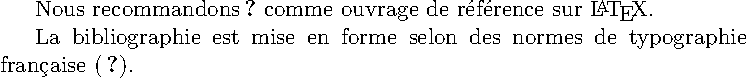
\includegraphics[width=\linewidth]{exemple-bibliographie-cropped-1}
    \end{framed}
    \code{xelatex} $\rightarrow$ \code{bibtex} $\rightarrow$ \code{xelatex}
    \begin{framed}
      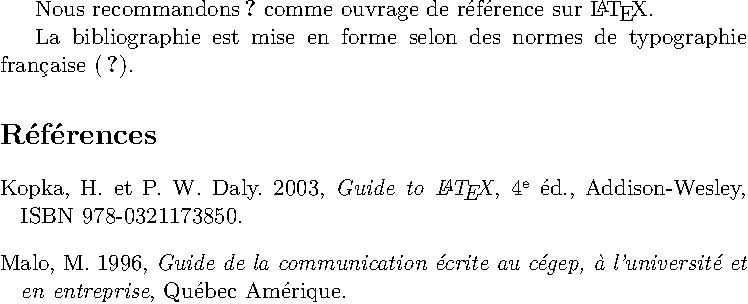
\includegraphics[width=\linewidth]{exemple-bibliographie-cropped-2}
    \end{framed}
    \code{xelatex} $\rightarrow$ \code{bibtex} $\rightarrow$ \code{xelatex} $\rightarrow$ \code{xelatex}
    \begin{framed}
      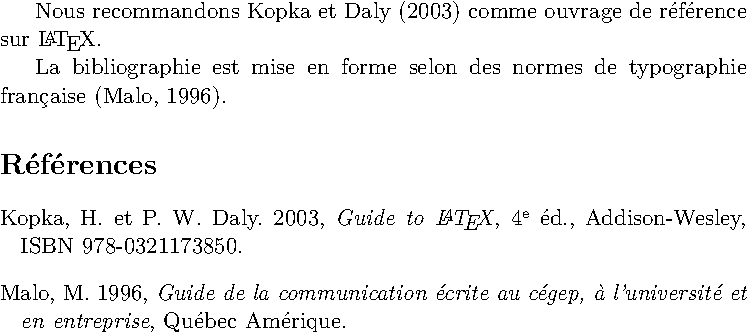
\includegraphics[width=\linewidth]{exemple-bibliographie-cropped-3}
    \end{framed}
    \caption{Zone de texte du document aux diverses étapes de la
      compilation des fichiers de la
      \autoref{fig:bibliographie:bibtex:1} avec {\XeLaTeX} et
      {\BibTeX}}
    \label{fig:bibliographie:bibtex:2}
  \end{figure}
\end{exemple}



Les éditeurs de texte spécialisés pour la préparation de documents
{\LaTeX} offrent généralement des raccourcis pour exécuter la
compilation avec {\BibTeX}.
\begin{itemize}
\item Dans TeXShop, on sélectionne un autre programme dans le menu à
  côté du bouton «Composition».
\item Dans Texmaker, on choisit le programme approprié dans le menu de
  composition rapide.
\end{itemize}
Ces deux interfaces sont représentées à la
\autoref{fig:bibliographie:editeurs}.

\begin{figure}
  \centering
  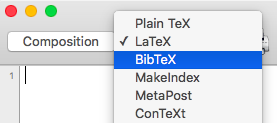
\includegraphics[height=2.2cm]{bibtex-texshop}
  \qquad
  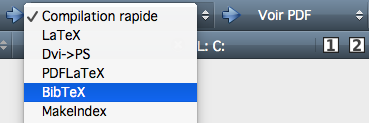
\includegraphics[height=2.2cm]{bibtex-texmaker}
  \caption{Interfaces de sélection du programme {\BibTeX} dans TeXShop
    (à gauche)
    et Texmaker (à droite)}
  \label{fig:bibliographie:editeurs}
\end{figure}

On trouvera des informations additionnelles, notamment sur des sources
de données bibliographiques et des outils de gestion des bases de
données, dans la section %
\doc[Gestion de la bibliographie]{}{https://fr.wikibooks.org/wiki/LaTeX/Gestion_de_la_bibliographie} %
de \citeauthor{wikilivres:latex}.

\begin{conseil}
  Aux toutes dernières étapes avant de rendre un document, s'assurer
  d'exécuter {\BibTeX} une dernière fois et de compiler avec
  pdf{\LaTeX} ou {\XeLaTeX} au moins deux fois. Le journal de la
  compilation (\emph{log file}) ne devrait pas rapporter de références
  manquantes (\emph{undefined references}).
\end{conseil}



%%%
%%% Exercices
%%%

\section{Exercices}
\label{sec:bibliographie:exercices}

\Opensolutionfile{solutions}[solutions-bibliographie]

\begin{Filesave}{solutions}
\section*{Chapitre \ref*{chap:bibliographie}}
\addcontentsline{toc}{section}{Chapitre \protect\ref*{chap:bibliographie}}

\end{Filesave}

\begin{exercice}
  toto
\end{exercice}

\Closesolutionfile{solutions}

%%% Local Variables:
%%% mode: latex
%%% TeX-engine: xetex
%%% TeX-master: "formation_latex-partie_2"
%%% coding: utf-8
%%% End:

%%% Copyright (C) 2018 Vincent Goulet
%%%
%%% Ce fichier fait partie du projet
%%% «Rédaction avec LaTeX»
%%% http://github.com/vigou3/formation-latex-ul
%%%
%%% Cette création est mise à disposition selon le contrat
%%% Attribution-Partage dans les mêmes conditions 4.0
%%% International de Creative Commons.
%%% http://creativecommons.org/licenses/by-sa/4.0/

\chapter{Commandes et environnements définis par l'usager}
\label{chap:commandes}

{\LaTeX} est un ensemble de macro-commandes conçu pour faciliter
l'utilisation du système {\TeX}. Dès lors, il est assez naturel de
permettre à l'usager de définir à son tour ses propres commandes. Il
suffit généralement d'avoir rédigé quelques documents --- ou quelques
chapitres d'un long document --- avec {\LaTeX} pour réaliser combien
cette possibilité est de nature à faciliter le travail.

La définition de nouvelles commandes et de nouveaux environnements
peut servir à créer des extensions à {\LaTeX} --- c'est d'ailleurs ce
que font plusieurs paquetages. Cependant, en usage courant, on fera
principalement appel à ces fonctionnalités pour l'une ou l'autre des
trois raisons suivantes:

\begin{enumerate}
\item créer des raccourcis pour de longues commandes utilisées
  fréquemment;
\item créer des commandes sémantiques afin d'uniformiser la
  présentation du texte;
\item modifier le comportement de commandes existantes --- car il est
  également possible de redéfinir une commande existante.
\end{enumerate}

\begin{exemple}
  \label{ex:commandes:intro}
  Nous avons créé ou modifié des commandes pour chacune des raisons
  ci-dessus dans la préparation du présent document.
  \begin{enumerate}
  \item Une nouvelle commande \cmdprint{\doc} facilite et systématise
    l'insertion de liens vers la documentation. D'un seul appel, elle
    crée un hyperlien dans le texte suivi de l'icône {\faExternalLink}
    et elle ajoute le nom du fichier de documentation dans la marge
    précédé de l'icône {\faBookmark}.
  \item Une nouvelle commande sémantique \cmdprint{\pkg} sert pour la
    mise en forme des noms de paquetages. Ainsi, leur présentation est
    toujours la même et si nous souhaitons en changer, il suffit de
    modifier la définition de la commande.
  \item La redéfinition de la commande \cmd{\chaptitlefont} de la
    classe \class{memoir} permet de modifier la police et la mise en
    forme des titres de chapitres.
  \end{enumerate}
  Nous reviendrons sur les détails de ces exemples dans la suite du
  chapitre. %
  \qed
\end{exemple}


\section{Nouvelles commandes}
\label{sec:commandes:commandes}

Les commandes \cmd{\newcommand} et \cmd{\renewcommand} permettent
respectivement de définir une nouvelle commande et de redéfinir une
commande existante --- c'est-à-dire d'en modifier la définition. On
place généralement les appels à ces commandes dans le préambule du
document.

\subsection{Commandes sans arguments}
\label{sec:commandes:commandes:sans_arg}

Certaines commandes ne requièrent pas d'argument; pensons à
\cmdprint{\LaTeX} ou \cmdprint{\bfseries}. Ce sont les commandes les
plus simples à créer. La syntaxe des commandes \cmd{\newcommand} et
\cmd{\renewcommand} pour de tels cas est la suivante:
\begin{lstlisting}
\newcommand{`\bs\meta{nom\_commande}'}`\marg{définition}'
\renewcommand{`\bs\meta{nom\_commande}'}`\marg{définition}'
\end{lstlisting}
Le premier argument, \bs\meta{nom\_commande}, est le nom de la
commande, avec le symbole \bs. Ce nom doit être différent de celui
de toute commande active\footnote{%
  Les commandes actives dans un document sont les commandes de base de
  {\TeX} et {\LaTeX} ainsi que les commandes de tous les paquetages
  chargés dans le préambule.} %
dans le document dans le cas de \cmdprint{\newcommand}. À l'inverse,
une commande active doit nécessairement porter le même nom lorsque
l'on fait appel à \cmdprint{\renewcommand}.

Le second argument, \meta{définition}, contient la définition de la
commande. Il peut s'agir de caractères à insérer dans le texte, de
commandes à exécuter ou d'une combinaison de tout cela.

\begin{exemple}
  La commande \cmd{\mathbb}, présentée à la
  \autoref{sec:math:symboles:mathcal}, permet de créer une lettre
  majuscule ajourée pour représenter un ensemble de nombres en
  mathématiques. Plutôt que de l'utiliser à divers endroits dans un
  document, il est préférable de définir une commande sémantique comme
  \cmdprint{\R} pour représenter l'ensemble des nombres réels:
\begin{lstlisting}
\newcommand{\R}{\mathbb{R}}
\end{lstlisting}
  Ainsi, si l'on souhaite pour une raison quelconque modifier la
  représentation de l'ensemble des nombres réels, il suffit de
  modifier la définition de la commande \cmdprint{\R} pour que le
  changement prenne effet dans tout le document. %
  \qed
\end{exemple}

\begin{exemple}
  Tel que mentionné à l'\autoref{ex:commandes:intro}, nous avons
  modifié la police des titres de chapitres dans le présent document
  en redéfinissant la commande \cmdprint{\chaptitlefont} de la classe
  \class{memoir}. Pour obtenir des titres de chapitres sans
  empattements, en caractères gras, de dimension \cmdprint{\Huge} et
  alignés à gauche, on trouve dans le préambule du document la
  déclaration
\begin{lstlisting}
\renewcommand{\chaptitlefont}{\normalfont%
  \sffamily\bfseries\Huge\raggedright}
\end{lstlisting}
  \qed
\end{exemple}


\subsection{Commandes avec arguments}
\label{sec:commandes:commandes:avec_arg}

Les commandes \cmdprint{\newcommand} et \cmdprint{\renewcommand} ont
d'autres tours dans leur sac. Leur syntaxe étendue permet également de
définir ou de redéfinir des commandes acceptant un ou plusieurs
arguments:
\begin{lstlisting}
\newcommand{`\bs\meta{nom\_commande}'}`\oarg{narg}\marg{définition}'
\renewcommand{`\bs\meta{nom\_commande}'}`\oarg{narg}\marg{définition}'
\end{lstlisting}
Le nouvel argument \meta{narg} est un nombre entre 1 et 9
spécifiant le nombre d'arguments de la commande. La \meta{définition}
de la commande doit alors contenir des jetons \code{\#1}, \code{\#2},
\dots\ pour identifier les endroits où les arguments 1, 2, \dots\
doivent apparaitre.

\begin{exemple}
  La nouvelle commande \cmdprint{\pkg} mentionnée à
  l'\autoref{ex:commandes:intro} affiche les noms de paquetages en
  caractères gras. La commande prend en argument le nom du paquetage.
  Sa définition est donc
\begin{lstlisting}
\newcommand{\pkg}[1]{\textbf{#1}}
\end{lstlisting}
  Il s'agit encore d'une commande sémantique permettant de changer
  aisément la mise en forme en modifiant une seule définition dans le
  préambule du document. %
  \qed
\end{exemple}

\begin{exemple}
  \label{ex:commandes:doc}
  La commande \cmdprint{\doc} mentionnée à
  l'\autoref{ex:commandes:intro} requiert trois arguments:
  \begin{enumerate}
  \item le texte de l'hyperlien qui sera placé au fil du texte;
  \item le nom du fichier de documentation à placer dans la marge dans
    une police non proportionnelle;
  \item l'URL vers le fichier de documentation en ligne.
  \end{enumerate}
  Voici une version simplifiée de la définition de la commande:
\begin{lstlisting}
\newcommand{\doc}[3]{%
  \href{#3}{#1~\raisebox{-0.2ex}{\faExternalLink}}%
  \marginpar{\faBookmark~\texttt{#2}}}
\end{lstlisting}
  La commande \cmd{\href} qui permet d'insérer un hyperlien dans le
  texte provient du paquetage \pkg{hyperref} \citep{hyperref}. Les
  commandes \cmdprint{\faEx\-ter\-nal\-Link} et \cmdprint{\faBookmark}
  proviennent du paquetage \pkg{fontawesome} \citep{fontawesome}; elles
  insèrent dans le texte des icônes de la police libre %
  \link{http://fortawesome.io/}{Font~Awesome}. %

  Avec la définition ci-dessus, la déclaration
\begin{lstlisting}
\doc{documentation}{hyperref}{%
  http://texdoc.net/pkg/hyperref}
\end{lstlisting}
  produit: \doc{hyperref}{http://texdoc.net/pkg/hyperref}. %
  \qed
\end{exemple}


\section{Nouveaux environnements}
\label{sec:commandes:environnements}

Tel que mentionné en introduction du chapitre, {\LaTeX} permet
également à l'utilisateur de définir ou de modifier des
environnements. La mécanique est similaire à celle de la définition de
commandes, sauf qu'un environnement compte trois parties: le début,
marqué par la déclaration \cmdprint{\begin\marg{...}} et, parfois, des
  commandes de configuration de l'environnement; le contenu en tant
  que tel; la fin, marquée par la déclaration
  \cmdprint{\end\marg{...}}.

On crée ou modifie des environnements avec les commandes
\begin{lstlisting}
\newenvironment`\marg{nom\_env}\oarg{narg}\marg{début\_déf}\marg{fin\_déf}'
\renewenvironment`\marg{nom\_env}\oarg{narg}\marg{début\_déf}\marg{fin\_déf}'
\end{lstlisting}
Les nombreux arguments sont les suivants:
\begin{list}{}{%
    \setlength{\labelsep}{1.5ex}
    \settowidth{\labelwidth}{\meta{début\_déf}}
    \setlength{\leftmargin}{\labelwidth}
    \addtolength{\leftmargin}{\labelsep}
    \setlength{\parsep}{0.5ex plus0.2ex minus0.2ex}
    \setlength{\itemsep}{0.3ex}
    \renewcommand{\makelabel}[1]{\meta{#1}\hfill}}
%

\item[nom\_env] nom de l'environnement à créer ou à modifier.
  Il est fortement recommandé de ne pas modifier les environnements de
  base de {\LaTeX};
\item[narg] un nombre entre 1 et 9 représentant le nombre
  d'arguments de l'environnement, lorsqu'il y en a. Les arguments sont
  utilisés de la même manière que dans les définitions de commandes;
\item[début\_déf] commandes et texte à insérer au début de
  l'environnement, lors de l'appel \cmdprint{\begin\marg{nom\_env}}.
  C'est dans ce bloc que doivent se trouver les jetons \code{\#1},
  \dots, \code{\#}\meta{narg} lorsque l'environnement a des
  arguments.
\item[fin\_déf] commandes et texte à insérer à la fin de
  l'environnement, lors de l'appel \cmdprint{\end\marg{nom\_env}}.
  \end{list}

\begin{exemple}
  \label{ex:commandes:citation}
  On souhaite composer les citations hors paragraphe de la
  manière suivante:
  \begin{quote}
    \small\itshape%
    Texte en italique, dans une police de taille inférieure au texte
    normal et en retrait des marges gauche et droite.
  \end{quote}
  Ceci est simple à réaliser en se basant sur l'environnement standard
  \Ie{quote} et en modifiant les attributs de police:
\begin{lstlisting}
\begin{quote}
  \small\itshape%
  Texte en italique...
\end{quote}
\end{lstlisting}

  Pour automatiquement composer toutes les citations de la même
  manière, il suffit de créer un nouvel environnement \Ie{citation}:
\begin{lstlisting}
\newenvironment{citation}%
  {\begin{quote}\small\itshape}%
  {\end{quote}}
\end{lstlisting}
  Le bloc de code ci-dessus peut ensuite être remplacé par
\begin{lstlisting}
\begin{citation}
  Texte en italique...
\end{citation}
\end{lstlisting}
  \qed
\end{exemple}

\tipbox{N'hésitez pas à créer des nouvelles commandes et des nouveaux
  environnements dès lors qu'une mise en forme particulière revient
  plus d'une ou deux fois dans un document.}



%%%
%%% Exercices
%%%

\section{Exercices}
\label{sec:commandes:exercices}

\Opensolutionfile{solutions}[solutions-commandes]

\begin{Filesave}{solutions}
\section*{Chapitre \ref*{chap:commandes}}
\addcontentsline{toc}{section}{Chapitre \protect\ref*{chap:commandes}}

\end{Filesave}

\begin{exercice}
  Certains auteurs composent les sigles et les acronymes\footnote{%
    Un sigle est une abréviation formée par une suite de lettres qui
    sont les initiales d'un groupe de mots. Un acronyme est un sigle
    qui se prononce comme un mot ordinaire.} %
  en petites capitales, avec ou sans les points: \textsc{c.q.f.d.},
  \textsc{nasa}.
  \begin{enumerate}
  \item Créer une commande \cmdprint{\NASA} qui insère l'acronyme
    \textsc{nasa} dans le texte. Rappelons que l'on compose du texte en petites
    capitales avec la commande \cmd{\textsc}.
  \item Créer une commande plus générale \cmdprint{\sigle} qui affiche
    son argument en petites capitales. La commande devra convertir
    l'argument en minuscules avec \cmd{\MakeLowercase} afin que le
    résultat soit toujours le même peu importe la casse utilisée dans
    le code. Ainsi, \lstinline=\sigle{nasa}=, \lstinline=\sigle{Nasa}= et
    \lstinline=\sigle{NASA}= donneront toujours
    \textsc{nasa}.
  \item Après avoir utilisé la commande \cmdprint{\sigle} à quelques
    reprises dans un document, modifier sa définition pour plutôt
    composer les sigles en majuscules.
  \end{enumerate}
  Utiliser le gabarit de document \fichier{exercice\_gabarit.tex} pour
  créer et tester les commandes ci-dessus.
  \begin{sol}
    \begin{enumerate}
    \item \lstinline=\newcommand{\NASA}{\textsc{nasa}}=
    \item \lstinline=\newcommand{\sigle}[1]{\textsc{\MakeLowercase{#1}}}=
    \item \lstinline=\newcommand{\sigle}[1]{\MakeUppercase{#1}}=
    \end{enumerate}
  \end{sol}
\end{exercice}

\begin{exercice}
  Nous n'avons pas abordé dans le chapitre une fonctionnalité plus
  avancée de \cmd{\newcommand} et \cmd{\renewcommand}, soit celle de
  pouvoir définir des commandes dont un argument est optionnel ou,
  plus précisément, de donner une valeur par défaut à un argument.

  La syntaxe réellement complète de \cmd{\newcommand} et
  \cmd{\renewcommand} est la suivante:
\begin{lstlisting}
\newcommand{`\bs\meta{nom\_commande}'}`\oarg{narg}\oarg{option}\marg{déf}'
\renewcommand{`\bs\meta{nom\_commande}'}`\oarg{narg}\oarg{option}\marg{déf}'
\end{lstlisting}
  L'argument additionnel \meta{option} contient la valeur par défaut
  du \emph{premier} argument de \bs\meta{nom\_commande}. Dès lors, la
  commande ne compte plus \meta{narg} arguments obligatoires, mais
  bien $\text{\meta{narg}} - 1$ arguments obligatoires et un optionnel.

  Modifier la définition de la commande \cmdprint{\doc} de
  l'\autoref{ex:commandes:doc} pour que «documentation» soit le texte
  par défaut de l'hyperlien qui est placé au fil du texte.
  \begin{sol}
    Avec la définition
\begin{lstlisting}
\newcommand{\doc}[3][documentation]{%
  \href{#3}{#1~\raisebox{-0.2ex}{\faExternalLink}}%
  \marginpar{\faBookmark~\texttt{#2}}}
\end{lstlisting}
    la déclaration à deux arguments
\begin{lstlisting}
\doc{hyperref}{http://texdoc.net/pkg/hyperref}
\end{lstlisting}
    produit toujours \doc{hyperref}{http://texdoc.net/pkg/hyperref}.
  \end{sol}
\end{exercice}

\begin{exercice}
  Modifier l'environnement \Ie{citation} de
  l'\autoref{ex:commandes:citation} afin de composer les citations
  hors paragraphe comme suit:
  \begin{quote}
    \begin{tabularx}{\linewidth}{X}
      \toprule
      \small\sffamily%
      La citation est toujours en retrait des marges gauche et droite,
      mais également surmontée et suivie de filets horizontaux. Le
      texte est en police de taille \cmdprint{\small}, droite et sans
      empattements. \\
      \bottomrule
    \end{tabularx}
  \end{quote}
  \emph{Astuce}: utiliser un tableau pleine largeur à l'intérieur de
  l'environnement \Pe{quote} pour disposer le texte et créer les
  filets horizontaux.
  \begin{sol}
    La définition suivante donne les résultats demandés:
\begin{lstlisting}
\newcommand{citation}
  {\begin{quote}
     \begin{tabularx}{\linewidth}{X}
       \toprule\small\sffamily}%
  {\\ \bottomrule
     \end{tabularx}
   \end{quote}}
\end{lstlisting}
    On remarquera dans le troisième argument la présence de la
    commande de fin de ligne {\bs\bs} qui doit absolument précéder
    \cmdprint{\bottomrule}.
  \end{sol}
\end{exercice}

\Closesolutionfile{solutions}

%%% Local Variables:
%%% mode: latex
%%% TeX-master: "formation-latex-ul"
%%% TeX-engine: xetex
%%% coding: utf-8
%%% End:

\chapter{Trucs et astuces divers}
\label{chap:trucs}

En clôture du document, ce chapitre traite de différents sujets que
même une personne débutant avec {\LaTeX} voudra assez rapidement
aborder, comme le contrôle des sauts de ligne et des sauts de page, la
modification de la police de caractère du document, l'utilisation de
la couleur ou l'insertion d'hyperliens dans le fichier de sortie PDF.
Nous offrons également de courtes introductions à des usages plus
spécialisés de {\LaTeX} comme la mise en page de code informatique, la
production de diapositives ou la programmation lettrée. Enfin, nous
expliquons sommairement comme assurer de manière efficace la gestion
des versions de ses documents, surtout dans un contexte de travail
collaboratif.

\section{Contrôle de la disposition du texte}
\label{sec:trucs:controle}

Des algorithmes élaborés permettent à {\LaTeX} de généralement
disposer le texte harmonieusement sur la page. Néanmoins, il
est parfois nécessaire  d'effectuer soi-même de menus ajustements,
notamment pour les sauts de page et la coupure de mots.

\subsection{Sauts de ligne et de page}
\label{sec:trucs:controle:sauts}

Il est assez rarement nécessaire avec {\LaTeX} de devoir forcer les
retours à la ligne. Chose certaine, l'on devrait toujours utiliser une
ligne blanche dans le code source pour identifier un changement de
paragraphe.

Cela dit, les commandes suivantes permettent d'insérer un saut de
ligne manuellement lorsque requis:
\begin{lstlisting}
\\
\\`\oarg{longueur}'
\newline
\end{lstlisting}
La commande {\pixbsbs} est connue: elle sert aussi à délimiter les
lignes dans les tableaux (\autoref{sec:tableaux:tableaux}) et les lignes
d'une suite d'équations (\autoref{sec:math:align}). L'argument optionnel
\oarg{longueur} permet d'insérer un blanc entre les deux lignes; la
\autoref{sec:boites:longueurs} explique comment spécifier une
longueur.

Généralement équivalente à {\bs\bs}, la commande \cmd{\newline} est
parfois nécessaire, notamment pour insérer un changement de ligne à
l'intérieur d'une cellule d'un tableau ou à l'intérieur d'un titre de
section. Quand {\bs\bs} ne fonctionne pas, essayer
\cmdprint{\newline}.

\begin{exemple}
  La commande {\bs\bs} est particulièrement utile --- voire nécessaire
  --- pour disposer des boîtes à l'intérieur d'une figure.
  L'utilisation de l'argument \meta{longueur} permet alors de
  contrôler l'espacement vertical entre les éléments. Comparer les
  deux exemples ci-dessous.
  \begin{demo}
    \begin{texample}[0.55\linewidth]
\begin{lstlisting}
\begin{minipage}{1.0\linewidth}
  \framebox[\linewidth]{texte}
\end{minipage} \\
\begin{minipage}{1.0\linewidth}
  \framebox[\linewidth]{texte}
\end{minipage}
\end{lstlisting}
      \producing
      \begin{minipage}{1.0\linewidth}
        \framebox[\linewidth]{texte}
      \end{minipage}
      \begin{minipage}{1.0\linewidth}
        \framebox[\linewidth]{texte}
      \end{minipage}
    \end{texample}

    \begin{texample}[0.55\linewidth]
\begin{lstlisting}
\begin{minipage}{1.0\linewidth}
  \framebox[\linewidth]{texte}
\end{minipage} \\`\textbf{[6pt]}'
\begin{minipage}{1.0\linewidth}
  \framebox[\linewidth]{texte}
\end{minipage}
\end{lstlisting}
      \producing
      \begin{minipage}{1.0\linewidth}
        \framebox[\linewidth]{texte}
      \end{minipage} \\[6pt]
      \begin{minipage}{1.0\linewidth}
        \framebox[\linewidth]{texte}
      \end{minipage}
    \end{texample}
  \end{demo}
  \qed
\end{exemple}

Les commandes
\begin{lstlisting}
\newpage
\clearpage
\cleartorecto              % classe memoir seulement
\cleartoverso              % classe memoir seulement
\end{lstlisting}
permettent d'insérer manuellement un saut de page pour éviter une
coupure malheureuse. La commande de base pour insérer un saut
n'importe où dans la page est \cmd{\newpage}. La commande
\cmd{\clearpage}, quant à elle, va également s'assurer d'afficher tous
les éléments flottants (\autoref{sec:tableaux:floats}) en attente de
disposition.

Les commandes \cmd{\cleartorecto} et \cmd{\cleartoverso}, propres à la
classe \class{memoir} permettent respectivement de passer
automatiquement à une page recto ou une page verso. Évidemment, elles
n'ont d'utilité que dans les documents recto-verso.

Moins directives, les commandes
\begin{lstlisting}
\pagebreak`\oarg{n}'
\enlargethispage`\marg{longueur}'
\end{lstlisting}
permettent de seulement aider {\LaTeX} à gérer les sauts de page à un
endroit précis. La commande \cmd{\pagebreak} est intéressante
lorsqu'utilisée avec son argument optionnel \meta{n}: celui-ci
indique, par le biais d'un nombre entier entre 0 et 4, à quel point
nous \emph{recommandons} à {\LaTeX} d'insérer un saut de page à
l'endroit où la commande apparaît (0 étant une faible recommandation
et 4, une forte).

La commande \cmd{\enlargethispage}, comme son nom l'indique, permet
d'allonger une page de \meta{longueur} pour y faire tenir plus de
texte. C'est une commande particulièrement utile pour éviter que la
toute dernière ligne d'un chapitre ou d'un document se retrouve seule sur
une page.

\subsection{Coupure de mots}
\label{sec:trucs:controle:coupure}

La coupure automatique des mots en fin de ligne est toujours active
avec {\LaTeX}. C'est d'ailleurs pourquoi il importe d'indiquer à
{\LaTeX} dans quelle langue est le texte (lorsque ce n'est pas en
anglais) avec les commandes du paquetage \pkg{babel}.

Il existe deux façons de contrôler la coupure de mots. La première,
principalement utilisée lorsque {\LaTeX} refuse de couper un mot en
fin de ligne, consiste à insérer des \emph{suggestions} d'endroits où
couper le mot avec la commande \cmd{\-}. Par exemple, en écrivant
\verb=vrai\-sem\-blance=, on indique à {\LaTeX} qu'il est possible de
diviser le mot en \emph{vrai-semblance} ou \emph{vraisem-blance}.

La seconde méthode, celle-là surtout utilisée lorsque {\LaTeX} ne
reconnaît pas des mots qui reviennent souvent dans le document,
consiste à fournir dans le préambule une liste d'exceptions avec la
commande
\begin{lstlisting}
\hyphenation`\marg{liste}'
\end{lstlisting}
La \meta{liste} est une suite de mots, séparés par des virgules, des
blancs ou des retours à la ligne, dans lesquels les points de coupure
sont identifiés par un trait d'union.

\begin{exemple}
  La commande suivante, insérée dans le préambule, permet d'ajouter
  des points de coupure aux mots «puisque», «constante» et
  «vraisemblance» pour l'ensemble du document.
\begin{lstlisting}
\hyphenation{puis-que,cons-tante,vrai-sem-blance}
\end{lstlisting}
  \qed
\end{exemple}

\begin{important}
  Règle générale, garder les opérations d'ajustements de la mise en
  page --- position des éléments flottants, sauts de page, lignes trop
  longues, etc. --- pour la toute fin de la rédaction.
\end{important}


\section{Polices de caractères: au-delà de Computer Modern}
\label{sec:trucs:police}

{\CM%
  Les documents {\LaTeX} standards sont facilement reconnaissables par
  leur police de caractères par défaut, Computer Modern --- celle
  utilisée dans ce paragraphe. Pour qui souhaitait briser la relative
  monotonie induite par cette uniformité, il a longtemps été difficile
  d'utiliser une autre police de caractères. Fort heureusement, la
  situation a beaucoup évolué et il est aujourd'hui assez simple de
  produire des documents {\LaTeX} utilisant des polices de caractères
  variées.}

Avant d'aller plus loin, une mise en garde: si votre document contient
plus que quelques équations mathématiques très simples, le choix de
police devient très restreint. La raison: peu de polices de caractères
comprennent des symboles mathématiques et les informations nécessaires
pour les assembler dans une mise en page satisfaisant les standards de
haute qualité usuels de {\LaTeX}.

Cela dit, pour qui souhaite aller au-delà de la police Computer Modern
sans trop se compliquer la vie, il existe deux solutions principales.

\begin{enumerate}
\item Utiliser l'une ou l'autre des polices PostScript standards.
  C'est très simple avec toute distribution {\LaTeX} moderne: il
  suffit de charger le paquetage approprié. Consulter la %
  \doc{psnfss2e}{http://texdoc.net/pkg/psnfss/} %
  de l'ensemble de paquetages PSNFSS pour connaître les choix
  disponibles.
\item Utiliser une police OpenType présente sur son système avec le
  moteur {\XeLaTeX}. Seule une poignée de ces polices offrent
  toutefois un support approprié pour les mathématiques. La gestion
  des polices de caractères avec {\XeLaTeX} se fait avec le paquetage
  standard \pkg{fontspec}; consulter sa %
  \doc{fontspec}{http://texdoc.net/pkg/fontspec/}.
\end{enumerate}

Pour les thèses et mémoires de l'Université Laval, la Faculté des
études supérieures et postdoctorales accepte les polices %
\begin{quote}
  \begin{tabbing}
    Computer Modern \qquad \=  ABCDEF abcdef 1234567890 \kill
    {\CM Computer Modern} \> {\CM ABCDEF abcdef 1234567890} \\
    {\Times Times} \> {\Times ABCDEF abcdef 1234567890} \\
    {\Palatino Palatino} \> {\Palatino ABCDEF abcdef 1234567890}
  \end{tabbing}
\end{quote}
Pour utiliser ces deux dernières avec {\LaTeX}, on charge
respectivement les paquetages \pkg{mathptmx} ou \pkg{mathpazo}. Avec
{\XeLaTeX}, on utilisera les polices Termes et Pagella du projet %
\link{http://www.gust.org.pl/projects/e-foundry/tex-gyre/}{TeX~Gyre}.
Ce sont des polices très similaires à Times et Palatino, disponibles
en version OpenType et qui fournissent un bon support pour les
mathématiques via le projet frère %
\link{http://www.gust.org.pl/projects/e-foundry/tg-math/}{TeX~Gyre Math}.

\begin{exemple}
  \label{ex:trucs:palatino}
  Pour utiliser la police PostScript classique Palatino avec {\LaTeX}
  tant pour le texte que pour les mathématiques, il suffit d'insérer
  dans le préambule de son document la commande
\begin{lstlisting}
\usepackage{mathpazo}
\end{lstlisting}

  Avec le moteur {\XeLaTeX}, il est possible d'utiliser n'importe
  quelle police de caractères OpenType et TrueType installée dans le
  système d'exploitation de l'ordinateur. Pour obtenir un résultat
  équivalent à celui de \pkg{mathpazo}, on installe les polices
  TeX~Gyre dans le système, puis on insère dans le préambule les
  commandes
\begin{lstlisting}
\usepackage{fontspec}
\setmainfont{TeX Gyre Pagella}
\setmathfont{TeX Gyre Pagella Math}
\end{lstlisting}
  \qed
\end{exemple}

Le texte principal du présent document est en %
\link{http://tug.org/store/lucida/}{Lucida Bright~OT}, %
une police commerciale de très haute qualité offrant également un
excellent support pour les mathématiques. Ses auteurs ont toujours été
proches de la communauté {\LaTeX}. La Bibliothèque de l'Université
Laval détient une licence d'utilisation de cette police. Les étudiants
et le personnel de l'Université peuvent s'en produrer une copie
gratuitement en écrivant à
\href{mailto:lucida@bibl.ulaval.ca}{lucida@bibl.ulaval.ca}.



\section{Couleurs}
\label{sec:trucs:couleurs}

L'utilisation de couleur dans un document {\LaTeX} requiert de charger
le paquetage \pkg{xcolor} \citep{xcolor}. Celui-ci définit d'abord
plusieurs couleurs que l'on peut utiliser directement; consulter la %
\doc{xcolor}{http://texdoc.net/pkg/xcolor} %
pour en connaître les différentes listes. Le
\autoref{tab:trucs:couleurs} fournit celle des couleurs toujours
disponibles.

\begin{table}
  \centering
  \caption{Couleurs toujours disponibles quand le paquetage
    \pkg{xcolor} est chargé}
  \label{tab:trucs:couleurs}
  \begin{tabularx}{1.0\linewidth}{XlXll}
    \toprule
    \fcolorbox{black}{black}{\phantom{xx}}\, black &
    \fcolorbox{black}{blue}{\phantom{xx}}\, blue &
    \fcolorbox{black}{brown}{\phantom{xx}}\, brown &
    \fcolorbox{black}{cyan}{\phantom{xx}}\, cyan &
    \fcolorbox{black}{darkgray}{\phantom{xx}}\, darkgray \\
    \addlinespace[3pt]
    \fcolorbox{black}{gray}{\phantom{xx}}\, gray &
    \fcolorbox{black}{green}{\phantom{xx}}\, green &
    \fcolorbox{black}{lightgray}{\phantom{xx}}\, lightgray &
    \fcolorbox{black}{lime}{\phantom{xx}}\, lime &
    \fcolorbox{black}{magenta}{\phantom{xx}}\, magenta \\
    \addlinespace[3pt]
    \fcolorbox{black}{olive}{\phantom{xx}}\, olive &
    \fcolorbox{black}{orange}{\phantom{xx}}\, orange &
    \fcolorbox{black}{pink}{\phantom{xx}}\, pink &
    \fcolorbox{black}{purple}{\phantom{xx}}\, purple &
    \fcolorbox{black}{red}{\phantom{xx}}\, red \\
    \addlinespace[3pt]
    \fcolorbox{black}{teal}{\phantom{xx}}\, teal &
    \fcolorbox{black}{violet}{\phantom{xx}}\, violet &
    \fcolorbox{black}{white}{\phantom{xx}}\, white &
    \fcolorbox{black}{yellow}{\phantom{xx}}\, yellow \\
    \bottomrule
  \end{tabularx}
\end{table}

On modifie la couleur du texte avec la commande
\begin{lstlisting}
\color`\marg{nom}'
\end{lstlisting}
où \meta{nom} est le nom d'une couleur. À moins de vouloir modifier la
couleur de tout ce qui suit, on limitera la portée de la commande par
des accolades.
\begin{demo}
  \begin{texample}
\begin{lstlisting}
texte {\color{red} en rouge}
et {\color{blue} en bleu}
\end{lstlisting}
  \producing
  texte {\color{red} en rouge} et {\color{blue} en bleu}
  \end{texample}
\end{demo}

La commande \cmd{\definecolor} permet de définir de nouvelles couleurs
selon plusieurs systèmes de codage. Le plus usuel demeure \emph{Rouge,
  vert, bleu} (RVB ou RGB, en anglais) où une couleur est représentée
par une combinaison de teintes --- exprimées par un nombre entre $0$
et $1$ --- de rouge, de vert et de bleu. Dans ce cas, la syntaxe de
\cmd{\definecolor} est
\begin{lstlisting}
\definecolor`\marg{nom}'{rgb}`\marg{valeur\_r,valeur\_v,valeur\_b}
\end{lstlisting}
où \meta{valeur\_r}, \meta{valeur\_v} et \meta{valeur\_b} sont
respectivement les teintes de rouge, de vert et de bleu.

\begin{exemple}
  La commande
\begin{lstlisting}
\definecolor{acier}{rgb}{0.1,0.4,0.6}
\end{lstlisting}
  définit une nouvelle couleur nommée \code{acier} composée de rouge
  30~\%, de vert 40~\% et de bleu 60~\%: %
  \fcolorbox{black}[rgb]{0.3,0,0}{\phantom{xx}} $+$ %
  \fcolorbox{black}[rgb]{0,0.4,0}{\phantom{xx}} $+$ %
  \fcolorbox{black}[rgb]{0,0,0.6}{\phantom{xx}} $=$ %
  \fcolorbox{black}[rgb]{0.3,0.4,0.6}{\phantom{xx}}. %
  On pourra utiliser la couleur \code{acier} directement dans la
  commande \cmdprint{\color}. %
  \qed
\end{exemple}

La commande \cmd{\colorlet}, dont la syntaxe simplifiée est
\begin{lstlisting}
\colorlet`\marg{nom}\marg{couleur}'
\end{lstlisting}
permet de faire référence à la \meta{couleur} déjà existante par
\meta{nom}. C'est pratique pour assigner un nom sémantique à une
couleur.



\section{Hyperliens et métadonnées de documents PDF}
\label{sec:trucs:hyperliens}

Nous en avons déjà traité à quelques reprises, notamment à la
section~4 de \citet{UL:latex:1}: le paquetage \pkg{hyperref}
\citep{hyperref} permet de transformer toutes les références dans le
texte en hyperliens cliquables lorsque le document est produit avec
pdf{\LaTeX} ou {\XeLaTeX}. C'est très pratique lors de la consultation
électronique d'un document.

Le paquetage offre une multitudes d'options de configuration; nous
n'en présenterons que quelques unes. On accède aux options de
configuration de \pkg{hyperref} via la commande \cmd{\hypersetup} dans
le préambule. Celle-ci prend en arguments des paires
\code{option=valeur} séparées par des virgules.

Une des principales choses que l'on pourra souhaiter configurer, c'est
le comportement et la couleur des divers types d'hyperliens. On
trouvera ci-dessous les options de configuration pertinentes, leur
valeur (avec en gras la valeur par défaut) ainsi qu'une brève
explication de chacune.

\begin{table}[h]
  \begin{tabularx}{1.0\linewidth}{@{}p{6em}p{6em}X@{}}
    \code{colorlinks} & \code{true}|\code{\textbf{false}} & colorer les
                                                            liens selon
                                                            leur type \\
    \code{linktocpage} & \code{true}|\code{\textbf{false}} & faire du
                                                             numéro de
                                                             page
                                                             plutôt que
                                                             du titre l'hyperlien dans
                                                             la table
                                                             des
                                                             matières \\
    \code{linkcolor} & \meta{couleur} & couleur des liens internes \\
    \code{urlcolor}  & \meta{couleur} & couleur des URL externes \\
    \code{citecolor} & \meta{couleur} & couleur des citations \\
    \code{allcolor}  & \meta{couleur} & couleur pour tous les types d'hyperliens
  \end{tabularx}
\end{table}

Lorsque la valeur admissible d'une option est \code{true} ou
\code{false}, sa seule mention équivaut à \code{true}. La valeur
\meta{couleur} est le nom d'une couleur telle que définie par
\pkg{xcolor} (\autoref{sec:trucs:couleurs}).

Les fichiers PDF peuvent contenir diverses métadonnées sur leur
contenu. Le paquetage \pkg{hyperref} permet de définir certaines
catégories de celles-ci, notamment les informations de document comme
le titre ou l'auteur. Nous ne mentionnons ici que deux options de
configutation; la section~3.7 de la %
\doc{hyperref}{http://texdoc.net/pkg/hyperref} %
contient la liste complète.

\begin{table}[h]
  \begin{tabularx}{1.0\linewidth}{@{}p{6em}p{6em}X@{}}
    \code{pdftitle}  & texte & titre du document PDF \\
    \code{pdfauthor} & texte & auteur du document PDF
  \end{tabularx}
\end{table}

\begin{exemple}
  \label{ex:trucs:couleurs}
  Le présent document fait appel aux définitions de couleurs
  et aux options de configuration de \pkg{hyperref} suivantes:
\begin{lstlisting}
\definecolor{link}{rgb}{0,0.4,0.6}   % ~RoyalBlue de dvips
\definecolor{url}{rgb}{0.6,0,0}      % rouge-brun
\definecolor{citation}{rgb}{0,0.5,0} % vert foncé
\hypersetup{colorlinks, linktocpage,
  linkcolor=link, urlcolor=url, citecolor=citation,
  pdftitle={Rédaction de thèses et mémoires avec LaTeX -
            Partie II},
  pdfauthor={Université Laval}}
\end{lstlisting}
  \qed
\end{exemple}

\begin{exemple}
  Les gabarits de thèses et de mémoires livrés avec la classe
  \class{ulthese} contiennent dans le préambule la ligne suivante:
\begin{lstlisting}
\hypersetup{colorlinks,allcolors=ULlinkcolor}
\end{lstlisting}
  Tous les liens de la thèse ou du mémoire seront donc de la même
  couleur, \code{ULlinkcolor} \fcolorbox{black}{ULlinkcolor}{\phantom{xx}},
  une couleur définie par la classe. %
  \qed
\end{exemple}

\begin{conseil}
  L'interaction du paquetage \pkg{hyperref} avec les autres est
  parfois (voire souvent) délicate. Pour cette raison, il est
  fortement recommandé de charger \pkg{hyperref} en tout dernier
  dans dans le préambule.
\end{conseil}



\section{Présentation de code informatique}
\label{sec:trucs:listings}

L'environnement standard \Ie{verbatim} de {\LaTeX} permet de présenter
du texte exactement tel qu'il est entré dans le code source du
document. C'est un environnement particulièrement utile pour afficher
du code informatique puisque le texte est composé en police non
proportionnelle et que sa disposition exacte est respectée.

\begin{demo}
  \begin{texample}
\begin{lstlisting}[deletetexcs={int,include}]
\begin{verbatim}
/* Hello World en C */
#include <stdio.h>

int main()
{
    printf("Hello world\n");
    return 0;
}
\end{verbatim}
\end{lstlisting}
    \producing
\begin{verbatim}
/* Hello World en C */
#include <stdio.h>

int main()
{
    printf("Hello world\n");
    return 0;
}
\end{verbatim}
  \end{texample}
\end{demo}

Si un document doit contenir beaucoup de code informatique et que l'on
souhaite exercer un fin contrôle sur sa disposition et sa mise en
forme, il vaut mieux se tourner vers un paquetage spécialisé comme
\pkg{listings} \citep{listings}. La %
\doc{listings}{http://texdoc.net/pkg/listings} %
du paquetage compare ses fonctionnalités à celles de plusieurs autres
paquetages similaires.

Le paquetage \pkg{listings} peut effectuer automatiquement le marquage
des mots-clés de nombreux langages de programmation, ajouter des
numéros de ligne, importer du code de fichiers externes ou même
indexer les mots-clés des extraits de code. À titre d'illustration, en
utilisant l'environnement \Ie{lstlisting} de \pkg{listings} plutôt que
\Ie{verbatim}, l'extrait de code C ci-dessus pourrait se présenter
ainsi:
\begin{demo}
  \begin{texample}
    \begin{vglisting}
\begin{lstlisting}
/* Hello World en C */
#include <stdio.h>

int main()
{
  printf("Hello world\n");
  return 0;
}
\end{lstlisting}
    \end{vglisting}
    \producing
\begin{lstlisting}[language=C,%
  deletetexcs={int,include},
  frame=single,%
  backgroundcolor=\color{Azure2},%
  rulecolor=\color{black},%
  numbers=left,%
  numberstyle=\tiny\sffamily,%
  stringstyle=\color{orange}\itshape,%
  identifierstyle=\color{cyan}\mdseries,%
  xleftmargin=12pt,%
  keywordstyle=\color{blue}\bfseries,
  index=]
/* Hello World en C */
#include <stdio.h>

int main()
{
  printf("Hello world\n");
  return 0;
}
\end{lstlisting}
  \end{texample}
\end{demo}

Il serait trop long et nettement hors de la portée du présent document
d'expliquer les nombreuses fonctionnalités de \pkg{listings}.
Précisons simplement que le paquetage a servi pour en composer les
extraits de code {\LaTeX} et pour construire une grande partie de
l'index.

\begin{exemple}
  \label{ex:trucs:listings}
  Pour parvenir à la présentation des extraits de code source {\LaTeX}
  de ce document, le paquetage \pkg{listings} est configuré dans le
  préambule de la manière suivante:
\begin{lstlisting}
%% Couleurs
\definecolor{comments}{rgb}{0.7,0,0}

%% Configuration de listings
\lstset{language=[LaTeX]TeX,
  basicstyle=\ttfamily\NoAutoSpacing,
  keywordstyle=\mdseries,
  commentstyle=\color{comments}\slshape,
  extendedchars=true,
  showstringspaces=false,
  backgroundcolor=\color{LightYellow1},
  frame=lr, rulecolor=\color{LightYellow1},
  xleftmargin=3.4pt, xrightmargin=3.4pt}
\end{lstlisting}
  (La couleur \code{LightYellow1} est définie par \pkg{xcolor} lorsque
  le paquetage est chargé avec l'option \code{x11names}.)
  \qed
\end{exemple}

%%% Réactivation des mots-clés.
%\lstset{language=[LaTeX]TeX, moretexcs={int,include}}


\section{Production de rapports avec l'analyse intégrée}
\label{sec:trucs:sweave}

Les publications scientifiques reposent souvent sur une forme ou une
autre d'analyse numérique ou statistique, la production de code
informatique, une simulation stochastique, etc. La portion
développement et analyse est alors produite avec un certain outil
et la publication, avec un outil d'édition séparé --- {\LaTeX} pour ce
qui nous occupe. Or, tous les auteurs ont vécu cette situation: les
résultats de l'analyse changent et il faut modifier le rapport en
conséquence, refaire les tableaux et les graphiques, retracer cette
valeur isolée au fil du texte directement tirée de l'analyse\dots\
Seule la quantité de temps perdu rivalise avec le risque d'erreur.

Il existe pourtant une meilleure façon de travailler.

Cette meilleure façon de faire, tirée du concept de
\emph{programmation lettrée}, consiste à combiner dans un seul et même
document l'analyse et le rapport, puis de produire automatiquement une
partie du second à partir de la première.

Les utilisateurs du système statistique R bénéficient ici d'une mise
en œuvre simple et élégante du concept ci-dessus avec l'outil Sweave
\citep{Sweave}. Un fichier Sweave est à la base un document {\LaTeX}
dans lequel on a inséré du code R à l'intérieur de balises spéciales
utilisant la syntaxe \code{noweb} \citep{noweb}, comme ceci:
\begin{lstlisting}
\section{Commandes R}

L'utilisateur de R interagit avec l'interprète en entrant
des commandes à l'invite de commande:
<<>>=
2 + 3
pi
cos(pi/4)
@
La commande \verb=exp(1)= donne \Sexpr{exp(1)},
la valeur du nombre $e$.
\end{lstlisting}

Par convention, on enregistre un tel document sous un nom se terminant
par l'extension \code{.Rnw}. Sa compilation s'effectue
en deux étapes:
\begin{enumerate}
\item Le fichier \code{.Rnw} est passé à la commande \code{Sweave()}
  de R. Celle-ci retrace les extraits de code placés entre les balises
  \verb|<<>>=| et \verb|@| et les remplace par des environnements
  {\LaTeX} contenant, par défaut, les expressions R et leur résultat
  dans des environnements \Ie{Sinput} et \Ie{Soutput}. Elle évalue
  également les expressions R se trouvant dans les commandes
  \cmd{\Sexpr} pour les remplacer par leur résultat. Cela produit un
  fichier \code{.tex}:
\begin{lstlisting}
\section{Commandes R}

L'utilisateur de R interagit avec l'interprète en entrant
des commandes à l'invite de commande:
\begin{Schunk}
\begin{Sinput}
> 2 + 3
\end{Sinput}
\begin{Soutput}
[1] 5
\end{Soutput}
\begin{Sinput}
> pi
\end{Sinput}
\begin{Soutput}
[1] 3.141593
\end{Soutput}
\begin{Sinput}
> cos(pi/4)
\end{Sinput}
\begin{Soutput}
[1] 0.7071068
\end{Soutput}
\end{Schunk}
La commande \verb=exp(1)= donne 2.71828182845905,
la valeur du nombre $e$.
\end{lstlisting}
\item On compile le fichier \code{.tex} comme d'habitude.
\end{enumerate}

Sweave se révèle particulièrement utile pour créer des graphiques à
partir de R: tout ce que l'on doit conserver dans son fichier
\code{.Rnw}, c'est le code pour créer le graphique. Il est également
possible de contrôler l'exécution des blocs de code et l'affichage du
code source et des résultats par le biais d'options placées à
l'intérieur de la balise d'ouverture \verb|<<>>=|. Consulter la %
\link{http://leisch.userweb.mwn.de/Sweave/Sweave-manual.pdf}{documentation} %
de Sweave pour les détails.

\link{http://mpastell.com/pweave/}{Pweave} est un système similaire à
Sweave pour le langage Python.

Inspiré de Sweave, knitr \citep{knitr} permet également d'entrelacer
du code {\LaTeX} et du code R. Cet outil offre plus d'options de
traitement que Sweave, mais au prix d'une complexité accrue.

En terminant, rappelons que Sweave n'est qu'un exemple de système de
programmation lettrée. Il en existe plusieurs autres. Il appartient
dès lors au lecteur de trouver le système qui correspond le mieux à
ses besoins.

\begin{information}
  On doit le concept de programmation lettrée au créateur de {\TeX},
  Donald Knuth.  En fait, tout le code source de {\TeX} est écrit
  en programmation lettrée! La %
  \link{https://fr.wikipedia.org/wiki/Programmation_lettrée}{page Wikipedia} %
  consacrée au sujet offre un très bon survol de l'historique et de la
  nature du concept.

  Le lecteur intéressé pourra consulter, par exemple, le %
  \link{http://www.ctan.org/tex-archive/macros/latex/contrib/ulthese}{code source} %
  de la classe \class{ulthese}. La documentation de la classe, le
  code {\LaTeX}, les gabarits, tout se trouve entrelacé
  dans le seul fichier \code{ulthese.dtx}.
\end{information}

\newpage

\section{Diapositives}
\label{sec:trucs:diapositives}

Il n'est pas rare qu'une publication scientifique fasse l'objet d'une
présentation dans le cadre d'un colloque ou d'un séminaire. Lorsque le
texte a été rédigé avec {\LaTeX}, il est tout naturel de souhaiter le
réutiliser pour la préparation de diapositives --- surtout si le texte
comporte de nombreuses équations mathématiques qu'il serait
extrêmement long de retranscrire dans un logiciel de présentation
comme PowerPoint.

Fort heureusement, il est tout à fait possible de composer ses
diapositives avec {\LaTeX}. La classe standard \class{slides} produit
des diapositives élégantes, quoique minimalistes, qui conviendront à
l'auteur qui ne recherche rien de plus que du texte noir sur fond
blanc.

Cependant, l'outil devenu le standard \emph{de facto} pour la
production de diapositives est la classe \class{beamer}
\citep{beamer}. Celle-ci compte un grand nombre de thèmes et de
gabarits élaborés, rend très simple l'insertion d'animations d'une
diapositive à l'autre, gère automatiquement la table des matières
et\dots\ produit des diapositives en couleur!

Quelle que soit la classe utilisée, les diapositives produites avec
{\LaTeX} se présentent sous forme de fichier PDF. On les projète avec
une liseuse PDF en mode plein écran.

Nous n'irons pas plus loin sur le sujet dans ce document. Consulter
la %
\doc{beamer}{http://texdoc.net/pkg/beameruserguide} %
de \class{beamer} pour apprendre à utiliser la classe. Produire des
diapositives de grande qualité avec les gabarits fournis avec la
classe est simple et rapide.

Les diapositives de la première partie de la formation
\citep{UL:latex:1} ont été produites avec \class{beamer}.



\section{Gestion des versions et travail collaboratif}
\label{sec:trucs:cvs}

Vous travaillez à plusieurs sur un même fichier ou seul, mais de
plusieurs postes de travail différents. Quelle est la plus récente
version du fichier? Mon ajout fait hier dans le fichier a-t-il été
pris en compte par ma collègue aujourd'hui? Une modification apportée
au fichier n'est plus nécessaire; comment retourner en arrière
facilement?

Les informaticiens ont résolu ce genre de problèmes il y a des
dizaines d'années avec les systèmes de gestion de versions. Les
systèmes les plus populaires en ce moment sont Subversion
\citep{subversion} et Git \citep{git}.

Bien que développés à l'origine pour la gestion du code source de
logiciels, les systèmes de contrôle de versions conviennent
parfaitement pour les sources {\LaTeX}. L'utilisation d'un tel système
permet de:
\begin{itemize}
\item toujours savoir quelle est la plus récente version d'un fichier;
\item travailler à plusieurs personnes simultanément sur un même
  fichier;
\item revenir aisément à une version antérieure d'un fichier;
\item comparer deux versions d'un fichier pour connaître les
  modifications qui y ont été apportées;
\item gérer automatiquement les éventuels conflits de modification
  d'un fichier;
\item disposer en tout temps d'une copie de secours de son travail
  lorsque l'on a recours à un serveur central (obligatoire avec
  Subversion; optionnel avec Git\footnote{%
    Si ce n'est que pour le volet de sauvegarde, nous recommandons
    d'utiliser avec Git un dépôt central tel que
    \link{https://github.com}{GitHub}, un serveur public qui héberge
    déjà des millions de projets.}.)
\end{itemize}
Un système de gestion de versions est un outil qui permet d'augmenter
considérablement sa productivité ou celle de son équipe de
travail au moment de rédiger un ouvrage scientifique.

La %
\link{https://fr.wikipedia.org/wiki/Gestion_de_versions}{page Wikipedia} %
sur le sujet offre une bonne introduction aux systèmes de gestion de
versions. Les membres de la communauté de l'Université Laval qui
souhaitent mettre sur pied un dépôt pour un projet pourront
consulter leur équipe de soutien informatique facultaire.

\begin{information}
  La présente documentation est conservée dans un dépôt Subversion
  public d'où l'on peut toujours obtenir la plus récente version.
  Consulter la page des notices de copyright au début du document pour
  accéder au dépôt.
\end{information}



%%%
%%% Exercices
%%%

\section{Exercices}
\label{sec:trucs:exercices}

\Opensolutionfile{solutions}[solutions-trucs]

\begin{Filesave}{solutions}
\section*{Chapitre \ref*{chap:trucs}}
\addcontentsline{toc}{section}{Chapitre \protect\ref*{chap:trucs}}

\end{Filesave}

\noindent%
Pour les exercices
\nolink{\ref{exercice:trucs:1}}--\nolink{\ref{exercice:trucs:n}},
utiliser le fichier \fichier{exercices\_trucs.tex}. Celui-ci reprend
une partie de la documentation de la classe \class{ulthese}. De plus,
on remarquera que le document:
\begin{itemize}
\item doit être compilé avec pdf{\LaTeX} puisqu'il charge les
  paquetages \pkg{inputenc} et \pkg{fontenc};
\item définit des nouvelles commandes \cmdprint{\class} et
  \cmdprint{\fichier} pour composer, respectivement, les noms de
  classe et les noms de fichier;
\item utilise la commande \cmdprint{\doc} de
  l'\autoref{ex:commandes:doc};
\item charge le paquetage \pkg{hyperref}, ce qui transforme les titres
  de la table des matières, les renvois aux notes de bas de page et
  les liens externes en hyperliens.
\end{itemize}
\medskip

\begin{exercice}
  \label{exercice:trucs:1}
  Compiler et visualiser le fichier sans aucune modification. Le texte
  est composé dans la police par défaut Computer Modern.

  Ensuite, modifier le préambule du document pour composer le document
  dans la police Palatino, tel qu'expliqué à
  l'\autoref{ex:trucs:palatino}. Charger également le paquetage
  \pkg{helvet} afin d'utiliser Helvetica pour le texte en police sans
  empattements (\cmdprint{\textsf}).
  \begin{sol}
    On doit ajouter dans le préambule les commandes
\begin{lstlisting}
\usepackage{mathpazo}
\usepackage{helvet}
\end{lstlisting}
    La police Helvetica est très grande. Tel que mentionné dans la %
    \doc{psnfss2e}{http://texdoc.net/pkg/psnfss/} %
    de PSNFSS (section~4), il est généralement préférable de charger
    le paquetage \pkg{helvet} avec, par exemple,
\begin{lstlisting}
\usepackage[scaled=0.92]{helvet}
\end{lstlisting}
    pour que le texte en Helvetica se marie mieux à celui dans une
    autre police.
  \end{sol}
\end{exercice}

\begin{exercice}
  Configurer le paquetage \pkg{hyperref} pour que les hyperliens dans
  la table des matières soient ancrés aux numéros de page plutôt
  qu'aux titres de section.
  \begin{sol}
    Tel qu'expliqué à la \autoref{sec:trucs:hyperliens}, on doit
    insérer dans le préambule du document la commande
\begin{lstlisting}
\hypersetup{linktocpage=true}
\end{lstlisting}
    ou, plus simplement,
\begin{lstlisting}
\hypersetup{linktocpage}
\end{lstlisting}
  \end{sol}
\end{exercice}

\begin{exercice}
  Charger le paquetage \pkg{xcolor} et ajouter l'option
  \code{colorlinks} à \pkg{hyperref}, puis recompiler le document.
  Observer les changements.
  \begin{sol}
    En conservant l'ajout de l'exercice précédent, on a dans le
    préambule la commande
\begin{lstlisting}
\hypersetup{colorlinks, linktocpage}
\end{lstlisting}
    Les hyperliens se présentent maintenant en couleur selon les
    paramètres par défaut de \pkg{hyperref}.
  \end{sol}
\end{exercice}

\begin{exercice}
  En s'inspirant de l'\autoref{ex:trucs:couleurs}, modifier la couleur
  des liens internes et externes.
  \begin{sol}
    On peut soit utiliser des couleurs prédéfinies de \pkg{xcolor}
    (\autoref{tab:trucs:couleurs}), soit en  définir de nouvelles avec
    \cmd{\definecolor}. On fait ensuite appel aux couleurs choisies
    pour les options \code{linkcolor} (liens internes) et
    \code{urlcolor} (liens externes) de \pkg{hyperref}.

    Exemple utilisant des couleurs prédéfinies:
\begin{lstlisting}
\hypersetup{colorlinks, linktocpage,
  linkcolor=brown, urlcolor=blue}
\end{lstlisting}

    Exemple avec de nouvelles couleurs:
\begin{lstlisting}
\definecolor{link}{rgb}{0,0.4,0.6}
\definecolor{url}{rgb}{0.6,0,0}
\hypersetup{colorlinks, linktocpage,
  urlcolor=url, linkcolor=link}
\end{lstlisting}
  \end{sol}
\end{exercice}

\begin{exercice}
  \label{exercice:trucs:n}
  Charger le paquetage \pkg{listings} et modifier l'environnement
  \Pe{verbatim} que l'on trouve dans le document pour un environnement
  \Pe{lstlisting}. En s'inspirant de l'\autoref{ex:trucs:listings},
  configurer la présentation des extraits de code pour utiliser une
  police non proportionnelle (\cmdprint{\ttfamily}) et un arrière-plan
  de la couleur standard «lightgray».
  \begin{sol}
    S'il y avait plusieurs extraits de code dans le document, mieux
    vaudrait les configurer tous à l'identique dans le préambule du
    document avec
\begin{lstlisting}
\lstset{basicstyle=\ttfamily,
  backgroundcolor=\color{lightgray}}
\end{lstlisting}
    Ensuite,
\begin{vglisting}
\begin{lstlisting}
latex ulthese.ins
\end{lstlisting}
\end{vglisting}
    donne le résultat demandé.

    Pour un seul extrait, il est également possible de simplement
    charger le paquetage dans le préambule et d'effectuer la
    configuration à l'ouverture de l'environnement, comme ceci:
\begin{vglisting}
\begin{lstlisting}[basicstyle=\ttfamily,
  backgroundcolor=\color{lightgray}]
latex ulthese.ins
\end{lstlisting}
\end{vglisting}
  \end{sol}
\end{exercice}

\begin{exercice}[nosol]
  Accéder au dépôt qui héberge le code source de cette formation
  {\LaTeX} en suivant le lien à la page des notices de copyright.
  Télécharger le fichier maître de la première partie de la formation
  et ses fichiers auxiliaires:

  \medskip
  \begin{minipage}{\linewidth}
    \dirtree{%
      .1 formation\_latex-partie\_1.tex.
      .2 licence-partie\_1.tex.
      .2 colophon-partie\_1.tex.
      .2 exercice\_commandes-output.pdf.
      .2 renvoi.pdf.
      .2 renvoi\_avec\_ref.pdf.
      .2 renvoi\_avec\_autoref.pdf.
      .2 ponctuation.pdf.
    }
  \end{minipage}
  \medskip

  (Les lecteurs curieux pourront aussi installer sur leur poste de
  travail un %
  \link{http://subversion.apache.org/packages.html}{client Subversion} %
  et l'utiliser pour extraire l'ensemble des fichiers du dépôt.)

  Une fois les fichiers en main, examiner le code source du fichier
  maître. Il s'agit d'un document utilisant la classe \class{beamer}
  pour créer des diapositives.

  Désactiver (effacer ou mettre en commentaire) les lignes suivantes
  du préambule:
\begin{lstlisting}
\defaultfontfeatures{Ligatures=TeX,Scale=0.92}
\setmainfont{Lucida Bright OT}
\setsansfont{Lucida Sans OT}
\setmathfont{Lucida Bright Math OT}
\setmonofont{Lucida Grande Mono DK}
\newfontfamily\titles{Myriad Pro}
\end{lstlisting}
  et, plus loin dans le fichier,
\begin{lstlisting}
\setbeamerfont{frametitle}{family=\titles}
\end{lstlisting}
  Compiler ensuite le document avec {\XeLaTeX}. En comparant le code
  source et les diapositives, observer comment \class{beamer} peut
  afficher des listes une puce à la fois à partir d'un environnement
  \Pe{itemize} usuel une fois qu'on lui a ajouté une option
  \verb=[<+->]=.
\end{exercice}

\Closesolutionfile{solutions}


%%% Local Variables:
%%% mode: latex
%%% TeX-engine: xetex
%%% TeX-master: "formation_latex_UL-partie_2"
%%% coding: utf-8
%%% End:


\appendix
\chapter{Solutions des exercices}
\label{chap:solutions}

\input{solutions-boites}
\input{solutions-tableaux+figures}
\input{solutions-mathematiques}
\input{solutions-bibliographie}
\input{solutions-commandes}
\input{solutions-trucs}

%%% Local Variables:
%%% mode: latex
%%% TeX-master: "formation-latex-ul"
%%% coding: utf-8
%%% End:


\bibliography{formation_latex}

\cleardoublepage
\printindex

\cleartoverso

\thispagestyle{empty}
\vspace*{\fill}

\begingroup
\calccentering{\unitlength}
\begin{adjustwidth*}{\unitlength}{-\unitlength}
  \begin{flushleft}
    \small %
    Ce document a été produit avec le système de mise en page
    {\XeLaTeX} à partir de la classe \class{memoir}. Le texte
    principal est en Lucida Bright~OT 11~points, les mathématiques en
    Lucida Bright Math~OT, le code informatique en Lucida Grande
    Mono~DK et les titres en Adobe Myriad~Pro. Les icônes proviennent
    de la police Font~Awesome.
  \end{flushleft}
\end{adjustwidth*}
\endgroup
\vfill

%%% Local Variables:
%%% mode: latex
%%% TeX-engine: xetex
%%% TeX-master: "formation_latex_UL-partie_2"
%%% coding: utf-8
%%% End:


\cleartoverso

%% Page couverture arrière.
% \setkeys{Gin}{width=\paperwidth}
% 
\includepdf[pages=2]{couvertures}

\end{document}

%%% Local Variables:
%%% mode: latex
%%% TeX-engine: xetex
%%% TeX-master: t
%%% coding: utf-8
%%% End:
